
\documentclass[11pt]{report}

%% PACKAGES
\usepackage{graphicx}
\usepackage{verbatim}
\usepackage{url}
\usepackage[printonlyused]{acronym}
\usepackage[ruled]{algorithm}
\usepackage{amsmath,amssymb,amsfonts,amsthm}
\usepackage{overpic}
\usepackage{calc}
\usepackage{color}
%\usepackage{times}
%\usepackage{ragged2e}
 \usepackage[margin=1.0in]{geometry}
\usepackage[colorlinks=false]{hyperref}
\usepackage{textcomp}
\usepackage{cite}
\usepackage{mdwlist}
\usepackage{subfiles}
\usepackage{enumitem}
\usepackage{calc}
\usepackage{array}
\usepackage{units}
\usepackage{arydshln,leftidx,mathtools}
\usepackage[caption=false,font=footnotesize]{subfig}
\usepackage{relsize}
\usepackage{float}
\usepackage{makecell}
\usepackage{soul}
\usepackage[htt]{hyphenat}
\usepackage{xr}
\usepackage{placeins}

\usepackage{algorithm}
\usepackage[noend]{algpseudocode}

\setcounter{tocdepth}{4}
\setcounter{secnumdepth}{4}

\makeatletter
\let\@tmp\@xfloat     
\usepackage{fixltx2e}
\let\@xfloat\@tmp                    
\makeatother

\usepackage[subfigure]{tocloft}
\usepackage[singlespacing]{setspace}
%\usepackage[nodisplayskipstretch]{setspace}
%\setstretch{1.0}

%\renewcommand\cftsecafterpnum{\vskip\baselineskip}
%\renewcommand\cftsubsecafterpnum{\vskip\baselineskip}
%\renewcommand\cftsubsubsecafterpnum{\vskip\baselineskip}

%\usepackage{mathtools}
%\usepackage[framed]{mcode}

\usepackage{pgfplots}

\usepackage{cancel}

\usepackage{tikz}
\usetikzlibrary{calc,patterns,decorations.pathmorphing,decorations.markings,fit,backgrounds}

\usepackage[strict]{changepage} %use to manually place figs/tables to get them within the margins

\makeatletter
\g@addto@macro\normalsize{%
  \setlength\abovedisplayskip{0.25pt}
  \setlength\belowdisplayskip{0.25pt}
  \setlength\abovedisplayshortskip{0.25pt}
  \setlength\belowdisplayshortskip{0.25pt}
}
\makeatother



\setlength{\parskip}{\baselineskip}

%% GRAPHICS PATH
\graphicspath{{./pictures/pdf/}{./pictures/ps/}{./pictures/png/}}

%% TODO
\newcommand{\todo}[1]{\vspace{5 mm}\par \noindent \framebox{\begin{minipage}[c]{0.98 \columnwidth} \ttfamily\flushleft \textcolor{red}{#1}\end{minipage}}\vspace{5 mm}\par}

%% MACROS
\providecommand{\abs}[1]{\lvert#1\rvert}
\providecommand{\norm}[1]{\lVert#1\rVert}
\providecommand{\dualnorm}[1]{\norm{#1}_\ast}
\providecommand{\set}[1]{\lbrace\,#1\,\rbrace}
\providecommand{\cset}[2]{\lbrace\,{#1}\nobreak\mid\nobreak{#2}\,\rbrace}
\providecommand{\onevect}{\mathbf{1}}
\providecommand{\zerovect}{\mathbf{0}}
\providecommand{\field}[1]{\mathbb{#1}}
\providecommand{\C}{\field{C}}
\providecommand{\R}{\field{R}}
\providecommand{\polar}{\triangle}
\providecommand{\Cspace}{\mathcal{Q}}
\providecommand{\Fspace}{\mathcal{F}}
\providecommand{\free}{\text{\{}\mathsf{free}\text{\}}}
\providecommand{\iff}{\Leftrightarrow}
\providecommand{\qstart}{q_\text{initial}}
\providecommand{\qgoal}{q_\text{final}}
\providecommand{\contact}[1]{\Cspace_{#1}}
\providecommand{\feasible}[1]{\Fspace_{#1}}
\providecommand{\prob}[2]{p(#1|#2)}
\providecommand{\prior}[1]{p(#1)}
\providecommand{\Prob}[2]{P(#1|#2)}
\providecommand{\Prior}[1]{P(#1)}
\providecommand{\parenth}[1] {\left(#1\right)}
\providecommand{\braces}[1] {\left\{#1\right\}}
\providecommand{\micron}{\hbox{\textmu m}}

%% MATH FUNCTION NAMES
\DeclareMathOperator{\conv}{conv}
\DeclareMathOperator{\cone}{cone}
\DeclareMathOperator{\homog}{homog}
\DeclareMathOperator{\domain}{dom}
\DeclareMathOperator{\range}{range}
\DeclareMathOperator{\argmax}{arg\,max}
\DeclareMathOperator{\argmin}{arg\,min}
\DeclareMathOperator{\area}{area}
\DeclareMathOperator{\sign}{sign}
\DeclareMathOperator{\mathspan}{span}
\DeclareMathOperator{\sn}{sn}
\DeclareMathOperator{\cn}{cn}
\DeclareMathOperator{\dn}{dn}
\DeclareMathOperator*{\minimize}{minimize}

\DeclareMathOperator{\atan2}{atan2}

\newtheorem{theorem}{Theorem}
\newtheorem{lemma}[theorem]{Lemma}

%\setlength{\RaggedRightParindent}{2em}
%\setlength{\RaggedRightRightskip}{0pt plus 3em}
%\pagestyle{empty}




\title{{\Huge EMTGv9 Software Design Document}}
\vspace{0.5cm}
\author
{	 
	Jacob A. Englander \thanks{EMTG product development lead, NASA Goddard Space Flight Center, Flight Dynamics and Mission Design Branch Code 595},
	Donald H. Ellison \thanks{EMTG development team lead, NASA Goddard Space Flight Center, Flight Dynamics and Mission Design Branch Code 595},
	Kyle Hughes \thanks{EMTG test team lead, NASA Goddard Space Flight Center, Flight Dynamics and Mission Design Branch Code 595},\\
	Alec Mudek \thanks{EMTG test team member, NASA Goddard Space Flight Center, Flight Dynamics and Mission Design Branch Code 595},
	Sean Napier \thanks{EMTG test team member, NASA Goddard Space Flight Center, Flight Dynamics and Mission Design Branch Code 595},
	Bruno Victorino Sarli \thanks{EMTG test team member, NASA Goddard Space Flight Center, Flight Dynamics and Mission Design Branch Code 595},
	Noble Hatten \thanks{EMTG development team member, NASA Goddard Space Flight Center, Flight Dynamics and Mission Design Branch Code 595},
	Jeremy Knittel \thanks{EMTG development team member emeritus}
}
\vspace{0.5cm}

\date{}


\begin{document}

\begin{titlepage}
\maketitle


\begin{figure}[H]
	\centering
	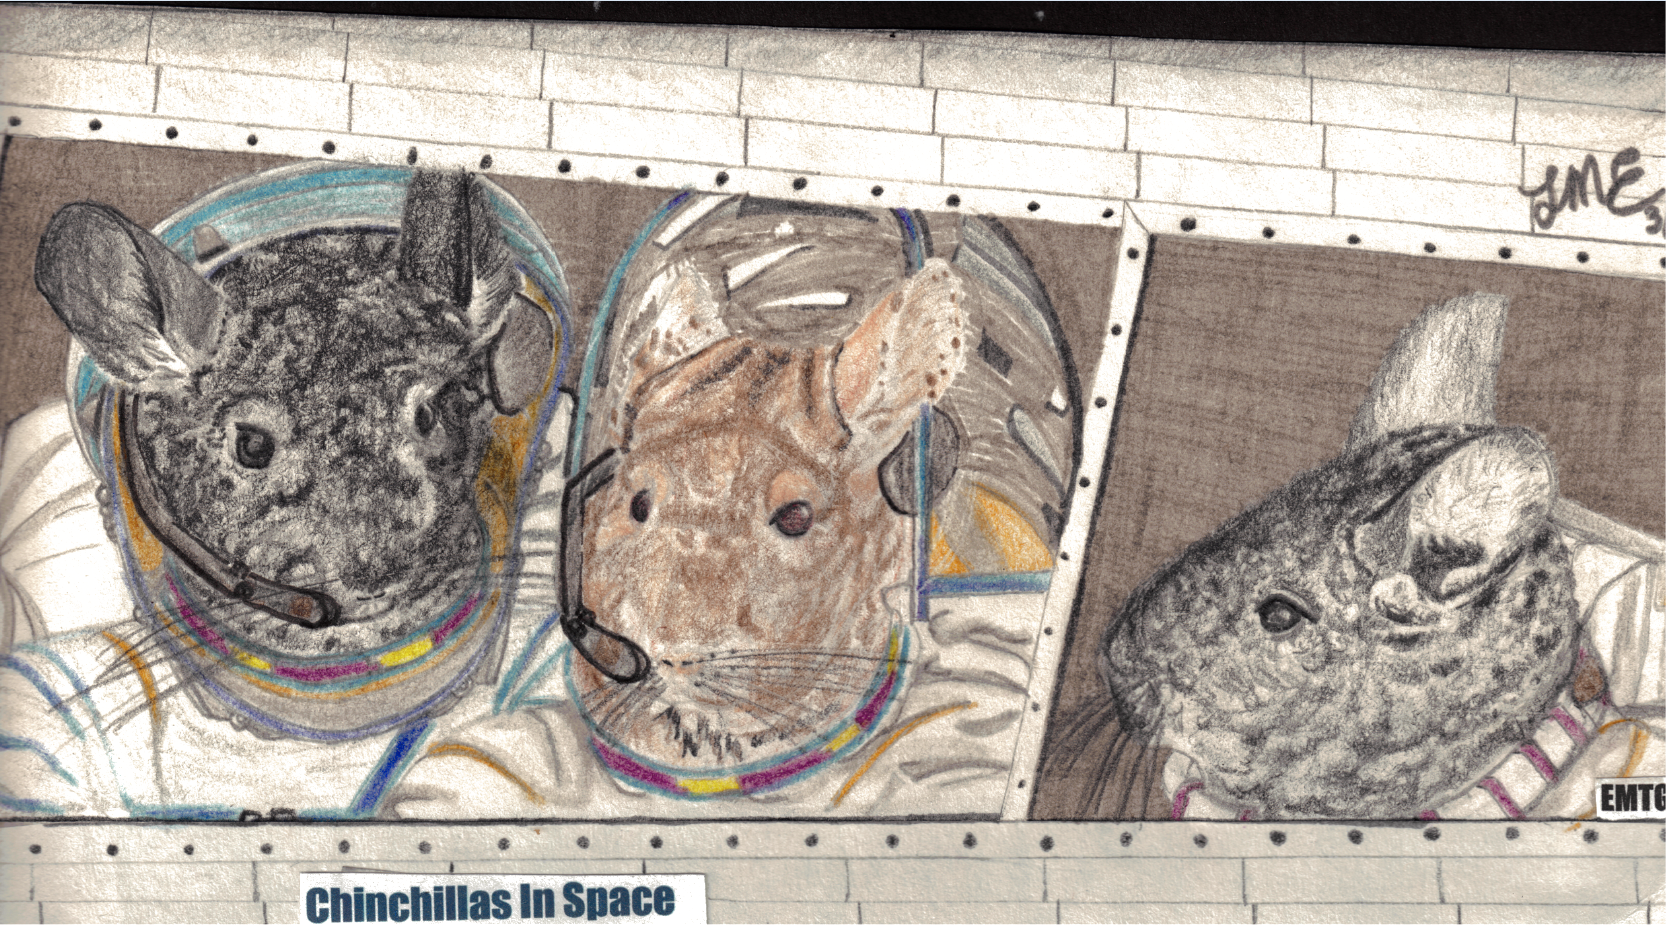
\includegraphics[width=0.75\linewidth]{./splashchilla.PNG}
\end{figure}

%\thispagestyle{empty}
\begin{table}[H]
	\centering
	\begin{tabular}{|l|l|l|}
		\hline
		\textbf{Revision Date} & \textbf{Author} & \textbf{Description of Change} \\ \hline
		\date{eventually} & us & first completed draft \\
		\hline
	\end{tabular}
\end{table}
\end{titlepage}



\tableofcontents
\clearpage
\listoffigures
\clearpage
\listoftables

\clearpage
\setcounter{page}{1}




\section*{List of Acronyms}
\begin{acronym}
%To define the acronym and include it in the list of acronyms: \acro{acronym}{definition}
%To define the acronym and exclude it from the list of acronyms:  \acro{acronym}{definition}
%
%\ac{acronym} Expand and identify the acronym the first time; use only the acronym thereafter
%\acf{acronym} Use the full name of the acronym.
%\{acronym} Use the acronym, even before the first corresponding \ac command
%\acl{acronym}  Expand the acronym without using the acronym itself.
%
%

\acro{ACS}{attitude control system}
\acro{ACO}{Ant Colony Optimization}
\acro{AD}{Automatic Differentiation}
\acro{ADL}{Architecture Design Laboratory}
\acro{AES}{Advanced Exploration Systems}
\acro{AGA}{aerogravity assist}
\acro{ALARA}{As Low As Reasonably Achievable}
\acro{API}{application programming interface}
\acro{BB}{branch and bound}
\acro{BVP}{Boundary Value Problem}
\acro{CATO}{Computer Algorithm for Trajectory Optimization}
\acro{CL}{confidence level}
\acro{CONOPS}{concept of operations}
\acro{COV}{Calculus of Variations}
\acro{D/AV}{Descent/Ascent Vehicle}
\acro{DE}{Differential Evolution}
\acro{DLA}{Declination of Launch Asymptote}
\acro{RLA}{Right Ascension of Launch Asymptote}
\acro{RA}{right ascension}
\acro{DEC}{declination}
\acro{DPTRAJ/ODP}{Double Precision Trajectory and Orbit Determination Program}
\acro{DSH}{Deep Space Habitat}
\acro{DSN}{Deep Space Network}
\acro{DSMPGA}{Dynamic-Size Multiple Population Genetic Algorithm}
\acro{EB}{Evolutionary Branching}
\acro{ECLSS}{environmental control and life support system}
\acro{ELV}{expendable launch vehicle}
\acro{EMME}{Earth to Mars, Mars to Earth}
\acro{EMMVE}{Earth to Mars, Mars to Venus to Earth}
\acro{EMTG}{Evolutionary Mission Trajectory Generator}
\acro{EVMME}{Earth to Venus to Mars, Mars to Earth}
\acro{EVMMVE}{Earth to Venus to Mars, Mars to Venus to Earth}
\acro{ERRV}{Earth Return Re-entry Vehicle}
\acro{FISO}{Future In-Space Operations}
\acro{FMT}{Fast Mars Transfer}
\acro{GASP}{Gravity Assist Space Pruning}
\acro{GCR}{galactic cosmic radiation}
\acro{GRASP}{Greedy Randomized Adaptive Search Procedure}
\acro{GSFC}{Goddard Space Flight Center}
\acro{GTOC}{Global Trajectory Optimization Competition}
\acro{GTOP}{Global Trajectory Optimization Problem}
\acro{HAT}{Human Architecture Team}
\acro{HGGA}{Hidden Genes Genetic Algorithm}
\acro{IMLEO}{Initial Mass in \acl{LEO}}
\acro{IPOPT}{Interior Point OPTimizer}
\acro{ISS}{International Space Station}
\acro{JHUAPL}{Johns Hopkins University Applied Physics Laboratory}
\acro{JSC}{Johnson Space Center}
\acro{KKT}{Karush-Kuhn-Tucker}
\acro{LEO}{Low Earth Orbit}
\acro{LRTS}{lazy race tree search}
\acro{MONTE}{Mission analysis, Operations, and Navigation Toolkit Environment}
\acro{MCTS}{Monte Carlo tree search}
\acro{MGA}{Multiple Gravity Assist}
\acro{MIRAGE}{Multiple Interferometric Ranging Analysis using GPS Ensemble}
\acro{MOGA}{Multi-Objective Genetic Algorithm}
\acro{MOSES}{Multiple Orbit Satellite Encounter Software}
\acro{MPI}{message passing interface}
\acro{MPLM}{Multi-Purpose Logistics Module}
\acro{MSFC}{Marshall Space Flight Center}
\acro{NELLS}{NASA Exhaustive Lambert Lattice Search}
\acro{NSGA}{Non-Dominated Sorting Genetic Algorithm}
\acro{NSGA-II}{Non-Dominated Sorting Genetic Algorithm II}
\acro{NHATS}{Near-Earth Object Human Space Flight Accessible Targets Study}
\acro{NTP}{Nuclear Thermal Propulsion}
\acro{OD}{orbit determination}
\acro{OOS}{On-Orbit Staging}
\acro{PCC}{Pork Chop Contour}
\acro{PEL}{permissible exposure limits}
\acro{PLATO}{PLAnetary Trajectory Optimization}
\acro{REID}{risk of exposure-induced death}
\acro{RTBP}{Restricted Three Body Problem}
\acro{SA}{Simulated Annealing}
\acro{SLS}{Space Launch System}
\acro{SNOPT}{Sparse Nonlinear OPTimizer}
\acro{SOI}{sphere of influence}
\acro{SPE}{solar particle events}
\acro{SQP}{sequential quadratic programming}
\acro{SRAG}{Space Radiation Analysis Group}
\acro{TEI}{Trans-Earth Injection}
\acro{TOF}{time of flight}
\acro{TPBVP}{Two Point Boundary Value Problem}
\acro{TMI}{Trans-Mars Injection}
\acro{VARITOP}{Variational calculus Trajectory Optimization Program}
\acro{VILM}{v-infinity leveraging maneuver}
\acro{MOI}{Mar Orbit Injection}
\acro{PCM}{Pressurized Cargo Module}
\acro{STS}{Space Transportation System}
\acro{EDS}{Earth Departure Stage}
\acro{NEO}{near-Earth asteroid}
\acro{IDC}{Integrated Design Center}
\acro{SEP}{solar-electric propulsion}
\acro{SRP}{solar radiation pressure}
\acro{NEP}{nuclear-electric propulsion}
\acro{REP}{radioisotope-electric propulsion}
\acro{DRM}{Design Reference Missions}

\acro{EDL}{entry, descent, and landing}
\acro{ASCII}{American Standard Code for Information Interchange}
\acro{AU}{Astronomical Unit}
\acro{BWG}{Beam Waveguides}
\acro{CCB}{Configuration Control Board}
\acro{CMO}{Configuration Management Office}
\acro{CODATA}{Committee on Data for Science and Technology}
\acro{DEEVE}{Dynamically Equivalent Equal Volume Ellipsoid}
\acro{DRA}{Design Reference Asteroid}
\acro{EME2000}{Earth Centered, Earth Mean Equator and Equinox of J2000 (Coordinate Frame)}
\acro{EOP}{Earth Orientation Parameters}
\acro{ET}{Ephemeris Time}
\acro{FDS}{Flight Dynamics System}
\acro{FTP}{File Transfer Protocol}
\acro{GSFC}{Goddard Space Flight Center}
\acro{PI}{Principal Investigator}
\acro{HEF}{High Efficiency}
\acro{IAG}{International Association of Geodesy}
\acro{IAU}{International Astronomical Union}
\acro{IERS}{International Earth Rotation and Reference Systems Service}
\acro{ICRF}{International Celestial Reference Frame}
\acro{ITRF}{International Terrestrial Reference System}
\acro{IOM}{Interoffice Memorandum}
\acro{JD}{Julian Date}
\acro{JPL}{Jet Propulsion Laboratory}
\acro{LM}{Lockheed Martin}
%\acro{LP150Q}{}
%\acros{LP100K}{}
\acro{MAVEN}{Mars Atmosphere and Volatile EvolutioN}
\acro{MJD}{Modified Julian Date}
\acro{MOID}{Minimum Orbit Intersection Distance}
\acro{MPC}{Minor Planet Center}
\acro{NASA}{National Aeronautics and Space Administration}
\acro{NDOSL}{\ac{NASA} Directory of Station Locations}
\acro{NEA}{near-Earth asteroid}
\acro{NEO}{near-Earth object}
\acro{NIO}{Nav IO}
\acro{OSIRIS-REx}{Origins Spectral Interpretation Resource Identification Security-Regolith Explorer}
\acro{PHA}{Potentially Hazardous Asteroid}
\acro{PHO}{Potentially Hazardous Object}
\acro{SBDB}{Small-Body Database}
\acro{SI}{International System of Units}
\acro{SPICE}{Spacecraft Planet Instrument Camera-matrix Events}
\acro{SPK}{SPICE Kernel}
\acro{SRC}{Sample Return Capsule}
\acro{SSD}{Solar System Dynamics}
\acro{STK}{Systems Tool Kit}
\acro{TAI}{International Atomic Time}
\acro{TBD}{To Be Determined}
\acro{TBR}{To Be Reviewed}
\acro{TCB}{Barycentric Coordinate Time}
\acro{TDB}{Temps Dynamiques Barycentrique, Barycentric Dynamical Time}
\acro{TDT}{Terrestrial Dynamical Time}
\acro{TT}{Terrestrial Time}
\acro{URL}{Uniform Resource Locator}
\acro{UT}{Universal Time}
\acro{UT1}{Universal Time Corrected for Polar Motion}
\acro{UTC}{Coordinated Universal Time}
\acro{USNO}{U. S. Naval Observatory}
\acro{YORP}{Yarkovsky-O'Keefe-Radzievskii-Paddack}

\acro{NLP}{nonlinear program}
\acro{MBH}{monotonic basin hopping}
\acro{MBH-C}{monotonic basin hopping with Cauchy hops}
\acro{FBS}{forward-backward shooting}
\acro{MGALT}{Multiple Gravity Assist with Low-Thrust}
\acro{MGALTS}{Multiple Gravity Assist with Low-Thrust using the Sundman transformation}
\acro{MGA-1DSM}{Multiple Gravity Assist with One Deep Space Maneuver}
\acro{MGAnDSMs}{Multiple Gravity Assist with \textit{n} Deep-Space Maneuvers using Shooting}
\acro{PSFB}{Parallel Shooting with Finite-Burn}
\acro{PSBI}{Parallel Shooting with Bounded Impulses}
\acro{FBLT}{Finite-Burn Low-Thrust}
\acro{FBLTS}{Finite-Burn Low-Thrust using the Sundman transformation}
\acro{ESA}{European Space Agency}
\acro{ACT}{Advanced Concepts Team}
\acro{IRAD}{independent research and development}
\acro{Isp}[$\text{I}_{sp}$]{specific impulse}
\acro{C3}[$C_3$]{hyperbolic excess energy}
\acro{GA}{genetic algorithm}
\acro{GALLOP}{ Gravity Assisted Low-thrust Local Optimization Program}
\acro{MALTO}{Mission Analysis Low-Thrust Optimization}
\acro{PaGMO}{Parallel Global Multiobjective Optimizer}
\acro{FRA}{feasible region analysis}
\acro{CP}{conditional penalty}
\acro{HOC}{hybrid optimal control}
\acro{HOCP}{hybrid optimal control problem}
\acro{PSO}{particle swarm optimization}
\acro{SEPTOP}{Solar Electric Propulsion Trajectory Optimization Program}
\acro{STOUR}{Satellite Tour Design Program}
\acro{STOUR-LTGA}{Satellite Tour Design Program - Low Thrust, Gravity Assist}
\acro{PaGMO}{Parallel Global Multiobjective Optimizer}
\acro{SDC}{static/dynamic control}
\acro{DDP}{Differential Dynamic Programming}
\acro{HDDP}{Hybrid Differential Dynamic Programming}
\acro{ACT}{Advanced Concepts Team}
\acro{GMAT}{General Mission Analysis Toolkit}
\acro{BOL}{beginning of life}
\acro{EOL}{end of life}
\acro{KSC}{Kennedy Space Center}
\acro{VSI}{variable \ac{Isp}}
\acro{RTG}{radioisotope thermal generator}
\acro{ASRG}{advanced Stirling radiosotope generator}
\acro{ARRM}{Asteroid Robotic Redirect Mission}
\acro{AATS}{Alternative Architecture Trade Study}
\acro{PPU}{power processing unit}
\acro{STM}{state transition matrix}
\acro{MTM}{maneuver transition matrix}
\acro{HPTM}{half-phase transition matrix}
\acro{BCI}{body-centered inertial}
\acro{BCF}{body-centered fixed}
\acro{UTTR}{Utah Test and Training Range}
\acro{EPV}{equatorial projection of $\mathbf{v}_\infty$}
\acro{KBO}{Kuiper belt object}
\acro{DSM}{deep-space maneuver}
\acro{BPT}{body-probe-thrust}
\acro{4PL}{four parameter logistic}
\acro{BCF}{body-centered fixed}
\acro{COE}{classical orbit elements}
\acro{GSL}{Gnu Scientific Library}
\acro{NEXT}{NASA's Evolutionary Xenon Thruster}

\acro{SMA}{semi-major axis}
\acro{ECC}{eccentricity}

\acro{GSAD}{Ghosh Sparse Algorithmic Differentiation}

\end{acronym}

% --------------------------------------------------------------------------------------------------------------------------
% --------------------------------------------------------------------------------------------------------------------------


\chapter{Introduction}
\label{chap:introduction}

This document presents a conceptual overview of the \acl{EMTG} (\acs{EMTG}) design. Each functional unit of the program is described in text. This document is \textit{not} intended to be a mathematics specification.

This document is intended to be used side-by-side with the \ac{EMTG} Doxygen-generated documentation. The Software Design Document describes the functional units of the design, and the Doxygen output maps the design to the code.

\endinput

\chapter{Common Design Elements}
\label{chap:common}

\section{Internal Calculation Frame}
\label{sec:internal_calculation_frame}

All internal calculations in EMTG are performed in the \ac{ICRF} as defined in International Celestial Reference Frame (ICRF) as defined in the \ac{IAU} Cartographic Coordinates and Rotational Elements document \cite{IAU_cartographic_coordinates_2018} and in \ac{SPICE} \cite{SPICE}. SPICE\'s \texttt{J2000} frame is identical to ICRF. The frame is always centered on whatever celestial body or barycenter that is relevant to the calculation, \textit{i.e.} the Sun, the Earth, or any other body or point \textit{that can be defined in SPICE}.

In some cases, the user may specify states or constraints in frames other than ICRF, or request output in frames other than ICRF. EMTG handles state input and output in alternative frames by rotating into ICRF, performing the calculations, and then rotating back to the requested output frame only at the last moment before the output is printed. Constraints, as described in Sections \ref{sec:specialized_boundary_constraints}, \ref{subsubsec:MGAnDSMs_maneuver_constraints}, and \ref{subsubsec:MGAnDSMs_maneuver_constraints}, work differently in that the constraint objects rotate EMTG's internal state into the frame of the constraint. The latter case occurs only in the individual constraint objects and therefore the rotated states are never available to the rest of the program and there is no opportunity for confusion as to what frame EMTG is working in.

\section{Units}
\label{sec:units}

All internal calculations are performed in units of kilometers, kilograms, and seconds. If particular piece of code needs to use a different unit system, then conversion is performed at the point where it is necessary and not passed to other parts of the code. The most frequent use of non-standard units is in input and output functions.

\externaldocument{../mission/c-Mission}
\externaldocument{../mission/c-Phase}
\externaldocument{../ObjectiveFunctions/c-ObjectiveFunctions}
\externaldocument{../hardware\_models/c-hardware\_models}
\externaldocument{../integration/c-integration}
\externaldocument{../propagation/c-propagation}
\externaldocument{../inner_loop/c-inner_loop}

\chapter{Core}
\label{chap:core}

\section{EMTG enums}
\label{sec:EMTG_enums}

\texttt{EMTG\_enums.h} is where we keep the enums that define EMTG's various modes. These enums are used to control switches in various class constructors throughout the rest of EMTG. The enums are listed below.

The following enums define the structure of the problem:
\begin{itemize}
	\item \textbf{PhaseType} - allows the user to specify a phase type as defined in Chapter \ref{chap:phase}.
	\item \textbf{StateRepresentation} - allows the user to specify how a given state vector is described in the problem. This is used in parallel shooting transcriptions (Section \ref{sec:parallel_shooting_phase}) and in PeriapseBoundary and FreePointBoundary (Sections \ref{sec:freepointboundary} and \ref{sec:periapseboundary})
	\item \textbf{ObjectiveFunctionType} - defines the objective function type as defined in Chapter \ref{chap:ObjectiveFunctions}.
\end{itemize}

The following enums define the spacecraft:
\begin{itemize}
	\item \textbf{SpacecraftModelInputType} - defines whether EMTG reads the spacecraft model from a file, constructs it from library entries, or constructs it from entries in the \texttt{.emtgopt} file, as described in Chapter \ref{chap:hardware_models}.
	\item \textbf{SpacecraftBusPowerType} - defines the spacecraft bus power model as described in Chapter \ref{chap:hardware_models}.
	\item \textbf{SpacecraftPowerSupplyType} - defines the spacecraft power supply type (solar vs radioisotope/nuclear) as described in Chapter \ref{chap:hardware_models}.
	\item \textbf{SpacecraftPowerSupplyCurveType} - defines the spacecraft power supply curve type as described in Chapter \ref{chap:hardware_models}.
	\item \textbf{SpacecraftThrusterMode} - defines which type of model to use for a given thruster, as described in Chapter \ref{chap:hardware_models}.
	\item \textbf{ThrottleLogic} - defines which set of rules to use for determining the number of thrusters to fire, as described in Chapter \ref{chap:hardware_models}.
	\item \textbf{PropulsionSystemChoice} - determines which propulsion system (monoprop, biprop, or electric) the spacecraft uses for a given maneuver, as described in Chapter \ref{chap:hardware_models}.
\end{itemize}

The following enums define boundary events:
\begin{itemize}
	\item \textbf{BoundaryClass} - defines whether a given boundary event will be constructed as an \texttt{EphemerisPeggedBoundary}, \texttt{FreePointBoundary}, \texttt{EphemerisReferencedBoundary}, or \texttt{PeriapseBoundary}, as described in Chapter \ref{chap:boundary-conditions}.
	\item \textbf{DepartureType} - defines the type of a departure event, within its class, as described in Chapter \ref{chap:boundary-conditions}.
	\item \textbf{ArrivalType} - defines the type of a arrival event, within its class, as described in Chapter \ref{chap:boundary-conditions}.
\end{itemize}

The following enums control EMTG's physics engine:
\begin{itemize}
	\item \textbf{PropagatorType} - defines whether EMTG uses a Kepler or integrated propagator for a given propagation as described in Chapter \ref{chap:Propagation}.
	\item \textbf{IntegratorType} - defines whether EMTG uses a fixed-step or adaptive-step integrator for a given propagation as described in Chapter \ref{chap:integration}.
	\item \textbf{PropagationDomain} - defines whether EMTG uses time-domain or Sundman-domain integration for a given propagation as described in Chapter \ref{chap:integration}.
	\item \textbf{DutyCycleType} - defines whether EMTG uses averaged or ``realistic'' duty cycle for thrust arcs in the \ac{PSFB} transcription, as described in Section \ref{subsec:PSFB}.
	\item \textbf{ReferenceFrame} - defines the reference frame for a given calculation, as described in Section \ref{sec:frame}.
\end{itemize}

The following enums control EMTG's solvers:
\begin{itemize}
	\item \textbf{InnerLoopSolverType} - defines which inner-loop solver (NLP-only, MBH, textit{etc.}) will be used for this run of EMTG, as described in Chapter \ref{chap:solvers}.
	\item \textbf{NLPMode} - defines whether EMTG runs its NLP solver in feasible point, optimize, or filament finder mode as described in Chapter \ref{chap:solvers}.
\end{itemize}

\section{doubleType}
\label{sec:doubleType}

\texttt{doubleType.h} is a very simple header that can be included in any EMTG source file and enables the use of the \ac{GSAD} package. It checks to see if the \texttt{AD\_INSTRUMENTATION} compiler macro is set. If so, the \texttt{doubleType} macro is defined as \texttt{GSAD::adouble} and the \texttt{\_getValue} and \texttt{\_setValue(x, y)} macros are defined as \texttt{GSAD::adouble::getValue()} and \texttt{GSAD::adouble::setValue(x, y)} macros, respectively. If the \texttt{AD\_INSTRUMENTATION} compiler macro is \textit{not} set, then \texttt{doubleType} is defined as \texttt{double} and \texttt{\_getValue} and \texttt{\_setValue(x, y)} are defined as white space.

\texttt{doubleType.h}, while only 20 lines long, is the key piece of code that enables EMTG to be its own partial derivative checker.

\section{Chinchilla}
\label{sec:chinchilla}

\texttt{Chinchilla.h} is a splash screen that draws an ascii picture of Clementine, the mascot of the EMTG program.

\section{MissionOptions}
\label{sec:missionoptions}

The \texttt{MissionOptions} class reads and write the \texttt{.emtgopt} files that control EMTG. \texttt{MissionOptions} contains options that globally control EMTG, plus a vector of \texttt{JourneyOptions} objects that control each individual journey.

Because \texttt{MissionOptions} must be changed in several different places each time a new option is added, we chose to generated it using an auto-coder. The developer need only modify \texttt{OptionsOverhaul/list\_of\_missionoptions.csv} and then run \textit{PyEMTG/OptionsOverhaul/make\_EMTG\_missionoptions\_journeyoptions.py}. The auto-coder will then validate the .csv file to ensure that all necessary fields are present, and will then generate the \texttt{MissionOptions} and \texttt{JourneyOptions} classes in both C++ and Python. The fields of \texttt{MissionOptions} and \texttt{JourneyOptions} are defined in a .csv file because it is plain text and easy to configuration-manage via Git.

By default, \texttt{MissionOptions} will only write out a given option if it \textit{does not match its default value}. This way each \texttt{.emtgopt} file is as short and easy to read as possible.

\section{JourneyOptions}
\label{sec:journeyoptions}

The \texttt{JourneyOptions} class controls the construction and evaluation of each \texttt{Journey} object and owned \texttt{Phase} objects. Like \texttt{MissionOptions}, \texttt{JourneyOptions} is generated via an auto-coder. The same auto-coder generates both classes. Also like \texttt{MissionOptions}, \texttt{JourneyOptions} only writes out options that do \textit{not} take their default values.

\section{Problem}
\label{sec:problem}

The \texttt{Problem} class is a base class for all EMTG problem types. As of this writing, \texttt{mission} (Chapter \ref{chap:mission}) is the only derived class of \texttt{Problem} but we keep the \texttt{Problem} class in case this changes later.

The main purpose of the \texttt{Problem} class is to hold all of the fields necessary to interact with an \ac{NLP} problem solver, including the decision vector, constraint vector, bounds, Jacobian, and Jacobian sparsity pattern. In addition, \texttt{Problem} contains helper methods to check the infinity-norm of the constraint violation vector and to check the decision vector, constraint vector, and Jacobian for infinite or undefined values.

\chapter{Astrodynamics}
\label{chap:astrodynamics}

\hl{Donald}

\section{Universe}
\label{sec:universe}

The \texttt{Universe} class is the central storage class for all celestial body and ephemeris data required by EMTG. EMTG creates a single \texttt{Universe} object for each \texttt{Journey} in the EMTG mission shortly after the EMTG options file is parsed. An emtg\_universe file is passed to the \texttt{universe} constructor and parsed using the \texttt{load\_universe\_data} method. If \texttt{SplineEphem} \ref{chap:splineephem} is being used, then a \texttt{SplineEphem\_universe} is also created and passed to the \texttt{Universe} constructor so that a spline-smoothed ephemeris may be used. The \texttt{universe} constructor also creates a \texttt{CentralBody} object that corresponds to the central body specified in the emtg\_universe file. The \texttt{universe} objects that correspond to the \texttt{Journeys} in an EMTG mission are connected together in a singly-linked list, the current \texttt{universe} has a pointer to the next \texttt{universe} in the mission to facilitate SOI transitions across \texttt{EphemerisReferenced} boundary events. The \texttt{next\_universe} pointer is accessed via the \texttt{get\_nextUniverse()} method.

An EMTG \texttt{universe} mostly contains astrodynamics data pertaining to the \texttt{CentralBody} (\ref{sec:central_body}), whose geometric center serves as the center of propagation in EMTG. The \texttt{locate\_central\_body} method computes the Cartesian state of the \texttt{CentralBody} with respect to the Sun, and returns zero, if the \texttt{CentralBody} is the Sun. A \texttt{universe} also contains a vector of \texttt{Body} objects for each of the perturbation/flyby targets available in a .emtg\_universe file. A \texttt{Frame} object is constructed using the \texttt{CentralBody} IAU Euler rotation angles (\ref{sec:frame}) and their first time derivatives $\{\alpha, \dot{\alpha}, \delta, \dot{\delta}, W, \dot{W}\}$ that are specified in a .emtg\_universe file. Gas drag on a spacecraft due to the atmosphere of the \texttt{CentralBody} can be modeled as discussed in section \ref{sec:AerodynamicDragTerm}. To facilitate this, if it is required, an \texttt{atmosphere} object is constructed for each \texttt{universe} object that requires one. This is done shortly after the \texttt{universes} are assembled in the main \texttt{EMTG\_v9.cpp} execution method.

The \texttt{universe} also contains some of the scaling information used by EMTG when it assembles the NLP problem passed to the NLP solver. The \texttt{continuity\_constraint\_scale\_factors} container contains multiplicative scaling factors that are applied to all trajectory defect constraints that appear in EMTG's trajectory transcriptions. Position defects are multiplied by $1/LU$, where $LU$ is specified by the user in the emtg\_universe file. A time scaling unit $TU$ is computed using the \texttt{CentralBody} $\mu$ and the provided $LU$. Velocity defects are multiplied by $TU/LU$. Mass defects are multiplied by $1/MU$ where $MU$ is the upper bound on the spacecraft's initial mass. Finally, time/epoch defects are multiplied by $1/TU$.


\section{Body}
\label{sec:body}

\hl{Donald}

Each \texttt{body} class owns a \texttt{frame} object and a \texttt{bplane} object.

\section{CentralBody}
\label{sec:central_body}



\section{Frame}
\label{sec:frame}

The \texttt{Frame} class handles transformations between EMTG's available reference frames. EMTG supports the following reference frames:

\begin{itemize}
	\item \textbf{\texttt{ICRF}}: A frame aligned with the International Celestial Reference Frame (ICRF) as defined in the \ac{IAU} Cartographic Coordinates and Rotational Elements document \cite{IAU_cartographic_coordinates_2018} and in \ac{SPICE} \cite{SPICE}. All of EMTG's internal calculations are performed in ICRF, so if the user specifies a state in some other frame, then the \texttt{frame} class has to transform it.
	
	\item \textbf{\texttt{J2000\_BCI (J2000 body-centered inertial)}}: A frame defined by the first two Euler rotations ($\alpha$ and $\delta$) in the \ac{IAU} Cartographic Coordinates and Rotational Elements document \cite{IAU_cartographic_coordinates_2018}, evaluated at January 1st, 2000 (J2000). This frame uses only the constant terms of the rotation, since the time-dependent terms are expressed as time since the J2000 epoch.
	
	\item \textbf{\texttt{J2000\_BCF (J2000 body-centered fixed)}}: A frame defined by a third Euler rotation beyond \texttt{J2000\_BCI} - a rotation about the \textit{z} axis by $W$ as defined in the \ac{IAU} Cartographic Coordinates and Rotational Elements document \cite{IAU_cartographic_coordinates_2018}. The first two rotations are evaluated at the J2000 epoch, but the $W$ rotation is evaluated at the epoch of the state being rotated. EMTGv9 only supports the linear component of the rotation, \textit{i.e} $W = W_0 + \dot{W}$. This was judged sufficient for EMTG's intended use cases. EMTG's \texttt{J2000\_BCF} is still an inertial frame; the time derivatives of the unit vectors of the \texttt{J2000\_BCF} frame are all zero. In other words, the position and velocity are rotated according to the IAU angles, but the velocity transformation does not include the $\mathbf{\omega} \times \mathbf{r}$ term. This is deliberate and is a definition that is often used for designing planetary probe trajectories. \hl{Kyle, Noble}
	
	\item \textbf{\texttt{TrueOfDate\_BCI (true-of-date body-centered inertial)}}: A frame identical to \texttt{J2000\_BCI} except that all three Euler rotations are evaluated at the epoch of the state being rotated.
	
	\item \textbf{\texttt{TrueOfDate\_BCF (true-of-date body-centered fixed)}}: A frame identical to \texttt{J2000\_BCF} except that all three Euler rotations are evaluated at the epoch of the state being rotated.
	
	\item \textbf{\texttt{PrincipleAxes}}: \hl{Noble}. Not yet fully implemented.
	
	\item \textbf{\texttt{Topocentric}}: \hl{Noble}. Not yet fully implemented.

	\item \textbf{\texttt{Polar}}: \hl{Noble}. Not yet fully implemented.
	
	\item \textbf{\texttt{J2000\_BCR (J2000 body-centered rotating)}}: A frame identical to \texttt{J2000\_BCF} except that the velocity vector is with respect to the rotating BCF frame. In other words, the $\mathbf{\omega} \times \mathbf{r}$ term is included, unlike in the \texttt{J2000\_BCF} frame. Not yet implemented.
	
	\item \textbf{\texttt{TrueOfDate\_BCR (true-of-date body-centered rotating)}}: A frame identical to \texttt{J2000\_BCR} except that all three Euler rotations are evaluated at the epoch of the state being rotated. Not yet implemented.
	
	\item \textbf{RIC (radial-intrack-crosstrack)}: A frame defined by the position and velocity vectors of the central body relative to some other reference body. For example, OSIRIS-REx uses a RIC frame where the \texttt{x} axis is the vector from the Sun to Bennu $\mathbf{r}$, the \texttt{z} axis is the angular momentum vector of Bennu about the sun $\mathbf{h} = \mathbf{r} \times \mathbf{v}$, and the \texttt{y} axis completes the right-handed set, $\mathbf{h} \times \mathbf{v}$. (not yet implemented)
	
	\item \textbf{SAM (sun-angular momentum, also called sun-north)}: The $x$ axis points from the central body to a reference body (\textit{i.e.} the Sun). The $y$ axis is the cross product of the \texttt{J2000BCI} spin pole and the $x$ axis. The $z$ axis complete the right-handed set.
	
	\item \textbf{Object-Referenced}: The $x$ axis points from the central body to the reference body. The $y$ axis is the velocity vector of the reference body relative to the central body. The $z$ axis completes the right-handed set and is the angular momentum vector of the reference body with respect to the central body. When this frame is used with a free point boundary condition, the first and second entries in the journey's destination list define the reference body for the departure and arrival event, respectively.
\end{itemize}

At construction, the owning object passes in the three Euler rotation angles and their first-order derivatives ($\alpha_0, \dot{\alpha}, \delta_0, \dot{\delta}, W, \dot{W}$). The \texttt{initialize\_J2000()} method is called by the constructor and creates the rotation matrices between \texttt{ICRF} and \texttt{J2000\_BCI}. These rotations are immediately available. The time-dependent transformations not evaluated immediately because the epoch of interest is not yet known. Instead, they are evaluated when the owning object, or another method of the \texttt{frame} itself, calls the \texttt{construct\_rotation\_matrices()} method. The rotations can be constructed with or without derivative information, as needed.

The owning object may then perform the transformation either by calling \textit{get\_R()} and \texttt{get\_dRdt} and performing the transformation outside the frame class, or more safely, by calling the \texttt{rotate\_frame\_to\_frame()} method. The \texttt{rotate\_frame\_to\_frame()} method performs the transformation and returns both the transformed state and its derivatives.

The \hl{\texttt{rotate\_frame\_to\_frame()} method will be the only safe way to transform to and from \texttt{Topocentric}, \texttt{Polar}, \texttt{J2000\_BCR}, and \texttt{TrueOfDate\_BCR} once they are fully implemented. We plan to force EMTG to use \texttt{rotate\_frame\_to\_frame()} everywhere, just to make sure.}

\section{StateRepresentation}
\label{sec:StateRepresentation}
The \texttt{StateRepresentation} set of classes handle the transformation between state representations. EMTG's default state representation is Cartesian. However there are times in various parts of the program where the user might specify state in another representation. This most frequently happens in \texttt{ParallelShootingStep} and \texttt{FreePointBoundary} but could be used in other places as well.

\texttt{StateRepresentationBase} is an abstract base class for state representation classes. A new derived class is written for every new state representation. These classes handle the transformation from Cartesian to the new state representation and back, and also compute the partial derivatives. It is up to the host class to put these partial derivatives into the Jacobian - \texttt{StateRepresentationBase} and its children just puts the math all in one place.

EMTG currently implements the following state representations, each of which has its own derived class:
\begin{itemize}
	\item Cartesian
	\item SphericalAZFPA
	\item SphericalRADEC
	\item Classical Orbit Elements (COE)
	\item B-plane coordinates $\left\{v_\infty, RHA, DHA, b_{radius}, b_{theta}, TA\right\}$. A full math spec is available in the ``bplane\_math.pdf'' file in the EMTG repository. Note that the b-plane reference vector for \texttt{IncomingBplaneRepresentation} is the current reference frame\'s $\hat z$ vector. It is not possible to make the reference vector depend on the state as that would result in a circular definition of the Cartesian state as a function of the b-plane coordinates.
\end{itemize}

\section{B-plane}
\label{sec:bplane}

\hl{Donald}

\section{AccelerationModel}
\label{sec:acceleration_model}

The \texttt{AccelerationModel} abstract base class establishes the interface between any derived acceleration models and EMTG's equations of motion classes (\ref{sec:Equations of Motion}) as well as any other entities that may have a need to directly it (MGALT with perturbations). The methods \texttt{AccelerationModel::setEpoch} and \texttt{AccelerationModel::setEpochJD} are used to set the current epoch (in seconds past the J2000 epoch and the Julian date in days respectively) to be used by any time-dependent acceleration terms (e.g. body rotational states, ephemeris-based gravity calculations, atmospheric drag). The \texttt{AccelerationModel::computeAcceleration} method takes a state vector and a boolean flag as its two inputs. The bool flag specifies whether the \texttt{AccelerationModel} should perform derivative computation. This method computes the instantaneous acceleration and stores the resultant \texttt{acceleration} vector. An overloaded for \texttt{computeAcceleration} can also be defined that accepts an input control vector should the \texttt{AccelerationModel} require a control term. The current acceleration vector can be extracted from the \texttt{AccelerationModel} using \texttt{AccelerationModel::getAcceleration}. The \texttt{AccelerationModel::populateInstrumentationFile} method must be implemented and should write acceleration data to the input \texttt{ofstream} for the input epoch (this method is also overloaded with a version that accepts a control vector as an input). 

\subsection{SpacecraftAccelerationModel}
\label{sec:spacecraft_acceleration_model}

The \texttt{SpacecraftAccelerationModel} class implements a Cartesian acceleration model for spacecraft motion with respect to the center of a gravitating body. A \texttt{SpacecraftAccelerationModel} can model the perturbative effects of $n$ third body gravity sources, spherical body solar radiation pressure, central body oblateness (J2) and gas drag assuming an exponential atmosphere model.

\begin{figure}[h!]
    \centering
    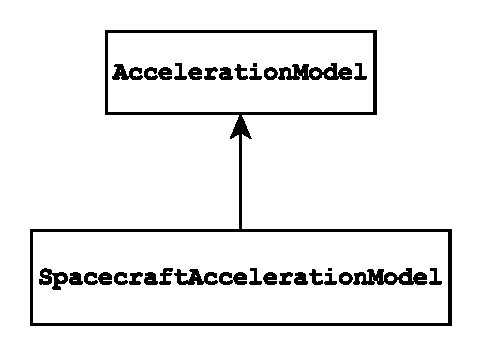
\includegraphics[width=0.3\linewidth]{./astrodynamics/AccelerationModel_inheritance.pdf}
    \caption{\label{fig:AccelerationModel_inheritance} AccelerationModel inheritance diagram.}
\end{figure} 

A \texttt{SpacecraftAccelerationModel} constructor requires pointers to a \texttt{MissionOptions} object, a \texttt{JourneyOptions} object, a \texttt{Universe} object, a vector of decision variable descriptions and a \texttt{Spacecraft} object. The input parameter \texttt{num\_STM\_size\_in} specifies the row and column dimensions the state propagation matrix that the acceleration model will compute. The boolean parameter \texttt{needCentralBody} indicates whether or not central body gravity should be included in the total acceleration calculation. This is useful for using a \texttt{SpacecraftAccelerationModel} to compute perturbations only (i.e. for an MGALT phase that models perturbation impulses, and accounts for two-body motion with respect to the central gravitating body using a \texttt{KeplerPropagator}).

On construction, the method \texttt{SpacecraftAccelerationModel::constructorInitialize} sizes various internal containers, tests if the acceleration is being computed in a heliocentric frame and then constructs whatever \texttt{SpacecraftAccelerationModelTerms} were requested by the user (via the \texttt{JourneyOptions} object pointer). During the construction of the individual \texttt{SpacecraftAccelerationModelTerms} the \texttt{needCentralBody} flag to determine if a \texttt{CentralBodyGravityTerm} is required. Calls to the \texttt{SpacecraftAccelerationModel} are categorized as heliocentric/non-heliocentric for the purposes of computing the distance from the sun for solar electric power calculations (non-heliocentric trajectories require an extra vector addition step and an associated ephemeris look-up to compute the sun-spacecraft distance).

The primary public method of the \texttt{SpacecraftAccelerationModel} is \texttt{SpacecraftAccelerationModel::computeAcceleration}, which computes and stores the acceleration experienced by the spacecraft. The inputs to this method are the spacecraft state vector, two flags indicating whether or not partial derivatives of the acceleration model should be computed and a control vector $\mathbf{u}$ (if the control overload is being called). Prior to calling this method, it is important to set the current epoch using \texttt{AccelerationModel::setEpoch} or \texttt{AccelerationModel::setEpochJD}. The majority of the public methods in \texttt{SpacecraftAccelerationModel} are get methods for extracting acceleration information from the model. These include \texttt{SpacecraftAccelerationModel::getAccelerationVec} (returns a vector of the total acceleration experienced by the spacecraft in the central body ICRF frame), \texttt{SpacecraftAccelerationModel::getGravityAccelerationVec} (returns a vector of the total gravitational acceleration on the spacecraft in the central body ICRF frame), \texttt{SpacecraftAccelerationModel::getGravityAccelSources} (returns a vector of 3-tuples, where each tuple contains a body name, body mu, and the acceleration of the spacecraft due to the body), \texttt{SpacecraftAccelerationModel::getSRPAccelerationVec} (returns the acceleration vector due to solar radiation pressure), \texttt{SpacecraftAccelerationModel::getThrustAccelerationVec} (returns the acceleration vector due to the spacecraft's thruster), \texttt{SpacecraftAccelerationModel::getThrusterMaxMassFlowRate} (returns the mass flow rate of the thruster), \texttt{SpacecraftAccelerationModel::getControlNorm} (returns the norm of the control parameters $u_x,~u_y,~u_z$), \texttt{SpacecraftAccelerationModel::getDutyCycle} (returns the duty cycle of the propulsion system), \texttt{SpacecraftAccelerationModel::getfx} (returns the state propagation matrix), \texttt{SpacecraftAccelerationModel::getSTMsize} (returns the row/column dimension of the state transition matrix), and \texttt{SpacecraftAccelerationModel::getCB2SC} (returns the distance from the central body to the spacecraft).

The \texttt{SpacecraftAccelerationModel::populateInstrumentationFile} method includes an overload with control and generates acceleration data for the current epoch and spacecraft state vector and writes it to the input \texttt{std::ofstream}. To do so, this method first writes the current JD epoch, the spacecraft state vector (including mass) and the total acceleration vector. Then, the method calls \texttt{SpacecraftAccelerationModelTerms::populateInstrumentationFile} for each term included in the acceleration calculation.

The private method \texttt{SpacecraftAccelerationModel::initializeAndComputeGeometry} zeros out the acceleration vector and the state propagation matrix (but sets the $\frac{\partial \mathbf{v}}{\partial \mathbf{v}}$ submatrix equal to $\mathbb{I}_{3\times3}$) and calls \texttt{SpacecraftAccelerationModel::computeScCbSunTriangle}. This method computes the position/velocity of the spacecraft w.r.t. the sun as well as the following partial derivative information:

\begin{align}
    &\frac{\partial \mathbf{r}_{\odot}}{\partial t} \label{eq:dr_sundepoch} \\
    &\frac{\partial \mathbf{r}_{\odot}}{\partial \Delta t_{\text{p}}} \label{eq:dr_sundflighttime}
\end{align},

\noindent where $\Delta t_{\text{p}}$ is the current phase flight time. If the trajectory is heliocentric, then Eq. (\ref{eq:dr_sundepoch}) and (\ref{eq:dr_sundflighttime}) are both zero.


\section{SpacecraftAccelerationModelTerm}
\label{sec:SpacecraftAccelerationModelTerm}

This is the abstract base class for the individual acceleration term classes in the \texttt{SpacecraftAccelerationModel}. Every \texttt{SpacecraftAccelerationModel} owns a \texttt{boost::ptr\_vector} of \texttt{SpacecraftAccelerationModelTerm} objects that are individually evaluated and polled for their contribution to the total acceleration acting on the spacecraft. The \texttt{SpacecraftAccelerationModelTerm} requires that each of its child classes define the following methods: \texttt{computeAccelerationTerm} (and its partial derivative overload), which evaluates the Cartesian acceleration contribution of the term, and \texttt{populateInstrumentationFile}, which writes acceleration data to the specified acceleration output file. The public accessor \texttt{getTermAcceleration} returns the computed acceleration contribution of the term. Each \texttt{SpacecraftAccelerationTerm} owns a member variable \texttt{SpacecraftAccelerationTerm::term\_acceleration}, which stores the acceleration contribution of the term and \texttt{SpacecraftAccelerationTerm::acceleration\_model}, which is a pointer to the \texttt{SpacecraftAccelerationModel} that owns the term object. Additional \texttt{SpacecraftAccelerationTerms} may be added to the \texttt{SpacecraftAccelerationModel} by creating them in the latter's constructor and adding their evaluation to \texttt{SpacecraftAccelerationModel::computeAcceleration}. The derived child classes that are currently implemented are described in the following subsections.

\subsection{GravityTerm}
\label{sec:GravityTerm}
\texttt{GravityTerm} contains the equations of motion that account for the acceleration due to the gravity of a point mass \texttt{Body} object on the spacecraft as well as on the \texttt{CentralBody} (center of integration). The \texttt{GravityTerm} constructor takes a pointer to its parent \texttt{SpacecraftAccelerationModel} and a pointer to the \texttt{Body} object whose gravity the class is modeling as input parameters.
The \texttt{computeAccelerationTerm} override calls the primary physics method \texttt{computePointMassGravityAcceleration} and then, if necessary, \texttt{computePointMassGravityDerivatives}. \\

The \texttt{computePointMassGravityAcceleration} method performs two main functions: 1) compute the position/velocity vectors between the \texttt{CentralBody}, the spacecraft and the gravitating point mass \texttt{Body} via a call to \texttt{computeScBodyCBtriangle} and 2) compute the acceleration on the spacecraft due to the gravitating \texttt{Body}. If the \texttt{GravityTerm} \texttt{Body} is the Sun, then the call to \texttt{computeScBodyCBtriangle} is skipped (to forgo an expensive ephemeris lookup call) as the \texttt{SpacecraftAccelerationBody::computeScCbSunTriangle} method has already been executed and has stored the position/velocity of the Sun w.r.t. the spacecraft and the \texttt{CentralBody}. Both the direct and indirect contributions of the gravity of the \texttt{Body} on the spacecraft are computed. The resultant point-mass gravity acceleration due to $i$ \texttt{Body} objects is computed in \texttt{SpacecraftAccelerationModel::computeAcceleration}:

\begin{equation}
\ddot{\mathbf{r}} = - \sum_{\text{i}} G~m_{\text{i}} \left( \frac{\mathbf{r} - \mathbf{r}_{\text{i}}}{\|\mathbf{r} - \mathbf{r}_{\text{i}}\|^3} + \frac{\mathbf{r}_{\text{i}}}{r_{\text{i}}^3} \right) \label{eq:EOM_point_mass_gravity} 
\end{equation}

\subsubsection{CentralBodyGravityTerm}
\label{sec:CentralBodyGravityTerm}

The \texttt{CentralBodyGravityTerm} class is derived from \texttt{GravityTerm} and is used to compute the acceleration of the (massless) spacecraft due to the gravity of the \texttt{CentralBody} whose geometric center coincides with the center of integration:

\begin{equation}
\ddot{\mathbf{r}} = -\frac{G \left(\cancelto{0}{m} + m_{\text{cb}}\right)}{r^2}\frac{\mathbf{r}}{r} \label{eq:EOM_central_body_gravity}
\end{equation}

The \texttt{CentralBodyGravityTerm} overrides the indirect gravitational effect of point mass gravity in \texttt{GravityTerm::computeFrameDragAcceleration} and sets that term equal to zero (since the center of integration is the center of the \texttt{CentralBody}, the \texttt{CenterBody} does not have a gravitational influence on itself, i.e. it has no trajectory w.r.t. the center of integration). The \texttt{GravityTerm::computePointMassGravityTimeDerivatives} method is similarly overrided and does nothing as the \texttt{CentralBody} gravity acceleration has no explicit time partials. \\

The \texttt{CentralBodyGravity} object also computes the acceleration on the spacecraft due to any \texttt{SphericalHarmonicTerms} that it owns in the \texttt{gravitational\_harmonic\_terms} \texttt{boost::ptr\_vector} container. At this time, only the J2 harmonic gravity term has been implemented, so the aforementioned container contains, at most, one \texttt{SphericalHarmonicTerm}.

\subsection{SphericalHarmonicTerm}
\label{sec:SphericalHarmonicTerm}
The \texttt{SphericalHarmonicTerm} class was designed to accommodate a spherical harmonic gravity model of arbitrary degree and order. Currently, only an oblateness model (J2) has been implemented. The \texttt{SphericalHarmonicTerm} constructor takes a pointer to the parent \texttt{SpacecraftAccelerationModel}, a pointer to the \texttt{Body} whose harmonic gravity this class is modeling, and a pointer to its parent/owner \texttt{CentralBodyGravityTerm}.

The \texttt{computeAccelerationTerm} method first extracts the position of the spacecraft w.r.t. the \texttt{CentralBody} by polling the \texttt{CentralBody} pointer. Next, it performs the following three actions: 1) rotate the spacecraft position into the true of date BCF frame 2) compute the acceleration due to the \texttt{CentralBody} oblateness 3) add the oblateness acceleration to the parent \texttt{CentralBody} \texttt{term\_acceleration} variable. The \texttt{computeAccelerationTerm(bool)} overload computes the acceleration due to \texttt{CentralBody} oblateness and its partial derivatives.

\begin{equation}
\label{eq:aBCFtoICRF}
\ddot{\mathbf{r}}_{J_2} = \ddot{\mathbf{r}}_{J_{2_{ICRF}}} = M^{ICRF}_{BCF}\ddot{\mathbf{r}}_{J_{2_{BCF}}}
\end{equation}

\begin{equation}
\ddot{\mathbf{r}}_{J_{2_{BCF}}} = \frac{3J_2 \mu R^2}{2r^5_{\text{BCF}}} \begin{bmatrix} 1 - 5\frac{x_{\text{BCF}}z^2_{\text{BCF}}}{r^2_{\text{BCF}}} \\ 1 - 5\frac{y_{\text{BCF}}z^2_{\text{BCF}}}{r^2_{\text{BCF}}} \\ 3 - 5\frac{z^3_{\text{BCF}}}{r^2_{\text{BCF}}} \end{bmatrix}
\end{equation}

\subsection{SolarRadiationPressureTerm}
\label{sec:SolarRadiationPressureTerm}

The \texttt{SolarRadiationPressureTerm} models spherical/cannonball solar radiation pressure. This term's constructor takes a pointer to its parent \texttt{SpacecraftAccelerationModel} as its only input parameter uses that pointer to extract the following parameters from the \texttt{MissionOptions} object: the spacecraft coefficient of reflectivity (SRP scale factor) $C_r$, the wetted surface area $A_s$, the illumination percentage $K$, solar irradiance $\phi$ at 1 AU (in $W/m^2$), and the speed of light in a vacuum $c$. The constructor also computes and stores the SRP coefficient:

\begin{equation}
C_{\text{SRP}} = \frac{C_r A_{s} K \phi}{c} \label{eq:SRP_coeff}
\end{equation}

The \texttt{computeAccelerationTerm} method calculates the instantaneous acceleration due to SRP, which is directed along the Sun-spacecraft line:

\begin{equation}
\ddot{\mathbf{r}} = C_{\text{SRP}}\frac{1}{m ~ r_{s/\odot}^2}\frac{\mathbf{r}_{s/\odot}}{r_{s/\odot}} \label{eq:EOM_SRP}
\end{equation}

\subsection{ThrustTerm}
\label{sec:ThrustTerm}

The \texttt{ThrustTerm} constructor takes a parent \texttt{SpacecraftAccelerationModel} pointer as its sole input in order to grant the class access to the \texttt{Spacecraft} (\ref{sec:spacecraft}) object to compute power system parameters, and the electric propulsion system performance parameters.

The \texttt{computeAccelerationTerm} method performs to actions to acquire the information it needs to compute the thruster acceleration 1) it extracts the control vector $\mathbf{u}$ from its parent \texttt{SpacecraftAccelerationModel} 2) the method requests that the \texttt{Spacecraft} object compute the current power system state and the electric propulsion system performance. The maximum thrust $T_{\text{max}}$ and maximum mass flow rate $\dot{m}_{\text{max}}$ are then extracted from the \texttt{Spacecraft} object. The acceleration due to the thrusters ($T_{\text{max}}$ accounts for the case when multiple thrusters are firing as well as any duty cycle that has been applied to the actual maximum thrust level) is then computed as follows:

\begin{equation}
\ddot{\mathbf{r}} = \frac{T_{\text{max}}}{m}\mathbf{u} \label{eq:EOM_thruster}
\end{equation}

\noindent Similarly, the mass flow rate is computed:

\begin{equation}
\dot{m} = - \|\mathbf{u}\| ~ \dot{m}_{\text{max}} \label{eq:EOM_m}
\end{equation}

If the \texttt{computeAccelerationTerm(bool)} overload is called, the \texttt{Spacecraft} model also provides partial derivative information for the power and thrust levels.

\subsection{AerodynamicDragTerm}
\label{sec:AerodynamicDragTerm}




\section{Equations of Motion}
\label{sec:Equations of Motion}

All equations of motion classes are instances of the Integrand class, which is operated on by an EMTG IntegrationScheme class in order to numerically integrate a state vector.

\begin{figure}[h!]
    \centering
    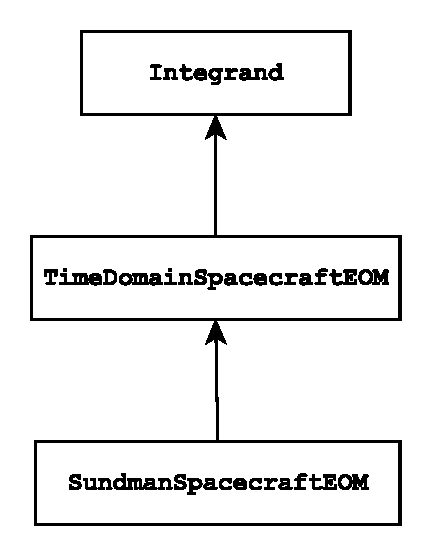
\includegraphics[width=0.3\linewidth]{./astrodynamics/Integrand_EOM_inheritance.pdf}
    \caption{\label{fig:Integrand_EOM_inheritance} Integrand inheritance diagram.}
\end{figure}

The \texttt{TimeDomainSpacecraftEOM} class encodes the first order Cartesian differential equations of motion using time as the independent variable and is derived from the \texttt{Integrand} class, which is called by implementations of the EMTG \texttt{IntegrationScheme} class. Specifically, an \texttt{IntegrationScheme} implementation calls the \texttt{TimeDomainSpacecraftEOM::evaluate} method in order to compute the current values of the differential equations (at a given epoch) as well as the orbit variational equations:

\begin{align}
\dot{\mathbf{r}} &= \mathbf{v} \label{eq:EOM_v}\\
\dot{\mathbf{v}} &= \mathbf{a} \label{eq:EOM_a} \\
\dot{m} &= -\|\mathbf{u}\|\dot{m}_{\text{max}} \label{eq:EOM_m} \\
\dot{t} &= 1 \label{eq:EOM_epoch} \\
\dot{f}_{\text{virt}} &= \dot{m}_{\text{ACS}} \label{eq:EOM_fuel} \\
\dot{o}_{\text{virt}} &= \|\mathbf{u}\|\dot{m}_{\text{max}} \label{eq:EOM_oxidizer} \\
\dot{\mathbf{\Phi}} &= \mathbf{A} \mathbf{\Phi} \label{eq:variational_eq},
\end{align}

\noindent where $\dot{m}_{\text{max}}$ is the maximum mass flow rate, $\mathbf{u} = \left[ u_x~~u_y~~uz \right]^T; \|\mathbf{u}\| \le 1$ is the maneuver control vector (\ref{subsec:TwoPointShootingLowThrustPhase}) $\mathbf{A} = \frac{\partial \dot{\mathbf{X}}}{\partial \mathbf{X}}$ is the state propagation matrix and $\mathbf{X} = \left[\mathbf{r} ~~ \mathbf{v} ~~ m ~~ t ~~ f_{\text{virt}} ~~ o_{\text{virt}} \right]^T$. Note that a differential equation is included for the current epoch $t$ (Eq. \ref{eq:EOM_epoch}), which is used to compute the current epoch if the independent variable of integration is not time (e.g. a Sundman propagator).

The \texttt{TimeDomainSpacecraftEOM::evaluate} method has two overloads, one for use with a control input, and one without (for ballistic trajectories). The \texttt{TimeDomainSpacecraftEOM::evaluate} method, first calls \texttt{TimeDomainSpacecraftEOM::computeAcceleration} (which has overloads for control/no control), which first sets the current epoch in the SpacecraftAccelerationModel and passes it pointers that it will use to extract time of flight and epoch partials from the SpacecraftAccelerationModel. Then, \texttt{TimeDomainSpacecraftEOM::computeAcceleration} calls \texttt{SpacecraftAccelerationModel::computeAcceleration}, which computes the instantaneous acceleration of the spacecraft and stores that vector. Next, \texttt{TimeDomainSpacecraftEOM::evaluate} calls \texttt{TimeDomainSpacecraftEOM::ballisticEOM}, the method that computes the first order differential equations of motion for ballistic flight. To do this, it extracts the current acceleration vector from the \texttt{SpacecraftAccelerationModel}. Despite the fact that it computes ballistic EOMs, this method also computes the differential equation for virtual chemical fuel if ACS usage is being tracked (section \ref{sec:propellant_and_dry_mass_constraints}). If the control overloaded \texttt{TimeDomainSpacecraftEOM::evaluate} is called, then \texttt{TimeDomainSpacecraftEOM::propulsionEOM} is called next, which computes the mass flow rate first order differential equations. Both overloads of \texttt{TimeDomainSpacecraftEOM::evaluate} set time derivative of current epoch (state vector entry 7) to 1.0, i.e. current epoch is (trivially) integrated, and it's time rate of change is 1.0. Finally, \texttt{TimeDomainSpacecraftEOM::evaluate} computes the variational equations by extracting the state propagation matrix from the SpacecraftAccelerationModel and computing the first order matrix differential equation.

The \texttt{SundmanDomainSpacecraftEOM} inherits from the \texttt{TimeDomainSpacecraftEOM} and applies the multiplicative transform to the t-domain EOM that transforms them to $\tau$-domain. It also computes the modified variational equations that account for this transformation:

\begin{align}
\mathring{\mathbf{X}} &= \frac{d\mathbf{X}}{d\tau} = \left( \frac{d\mathbf{X}}{dt} \right) \frac{dt}{d\tau} = \dot{\mathbf{X}}c_{\gamma} r^{\gamma} = \dot{\mathbf{X}}\eta\\
\mathring{\mathbf{\Phi}} &= \frac{\partial \mathring{\mathbf{X}}}{\partial \mathbf{X}} = \left( \frac{\partial \dot{\mathbf{X}}}{\partial \mathbf{X}}\eta + \dot{\mathbf{X}}\frac{\partial \eta}{\partial \mathbf{X}} \right) \mathbf{\Phi} = \left( \mathbf{A}\eta + \dot{\mathbf{X}}\frac{\partial \eta}{\partial \mathbf{X}} \right) \mathbf{\Phi}
\end{align}

\noindent where $\eta = c_{\gamma}r^{\gamma}$ is the multiplicative Sundman transformation function, $c_{\gamma}$ is a constant, which is set equal to the Universe length unit (LU), and $\gamma$ is the Sundman power constant, which is set to 1.0 in the current implementation. This means that the integration time steps correspond to a eccentric anomaly (to within a constant scale factor).






\externaldocument{../mission/c-Mission}
\externaldocument{../mission/c-phase}

\chapter{Hardware Models}
\label{chap:hardware_models}

\section{Overview}
\label{sec:hardware-overview}

All calculations in EMTGv9 that model the performance of hardware, \textit{i.e.} a launch vehicle or a spacecraft, are handled by \ac{EMTG}'s hardware classes. These classes are deliberately designed such that they can be used both by EMTG itself and by external programs. For example, the classes described in this chapter are also used by \ac{GMAT} and can also be compiled as a Python module.

The purpose of the separable hardware models is threefold. First, we wanted to create hardware models that could be used by many tools, not just EMTG. Second, we wanted a way to configuration manage spacecraft and launch vehicle properties just like we do ephemeris files. Third, we wanted all information about physical hardware to reside in text files that are not distributed with \ac{EMTG}. That way we can distribute \ac{EMTG} without any proprietary or ITAR/EAR restricted information.

\section{Launch Vehicle Model}
\label{sec:LaunchVehicle}

The \texttt{LaunchVehicle} class is responsible for calculating the performance (delivered mass) of a launch vehicle to an input \ac{C3} as well as the derivative of the delivered mass with respect to a changing \ac{C3}. \ac{EMTG} currently supports only a polnomial function of mass as a function of \ac{C3},

\begin{equation}
	m \left(C_3\right) = \left(1 - \eta_{LV}\right) \sum_{i=0}^{n} c_i C_3^i - m_{adapter}
	\label{eq:launch_vehicle_polynomial}
\end{equation}
%
where $\eta_{LV}$ is launch vehicle margin as specified in the user's .emtgopt mission script, the $c_i$ are coefficients associated with the particular launch vehicle, and $m_{adapter}$ is the launch vehicle adapter mass specified.

The \texttt{LaunchVehicle} class is designed such that additional launch vehicle models may be added at a later date.

\subsection{Launch Vehicle Library}
\label{subsec:LaunchVehicleLibrary}

The coefficients necessary to define a \texttt{LaunchVehicle}, as well as the upper and lower bounds on the validity of the performance polynomial and the upper and lower bounds on the \ac{DLA}, are held in a \texttt{LaunchVehicleOptions} object. A set of \texttt{LaunchVehicleOptions} objects are held in a \texttt{LaunchVehicleOptionsLibrary}.

\texttt{LaunchVehicleOptionsLibrary} reads a text file defining a set of launch vehicles. Each launch vehicle is associated with a ``launch vehicle key string.'' The user provides a key string to \ac{EMTG}, and \ac{EMTG} in turn passes the key string into the \texttt{LaunchVehicleOptionsLibrary} and returns the particular \texttt{LaunchVehicleOptions} object that the user wants. The \texttt{LaunchVehicleOptions} object is then passed as an argument to the constructor of \texttt{LaunchVehicle} to create the calculation object. The \texttt{LaunchVehicleOptionsFactory} function performs these steps.

\section{Spacecraft Model}
\label{sec:spacecraft}

The \texttt{Spacecraft} class handles all modeling of properties of the spacecraft propulsion and power system, as well as book-keeping of any propellant tank constraints. A spacecraft in \ac{EMTG} is composed of a number of stages. The primary job of the spacecraft class is to hold a vector of \texttt{Stage} objects as described in Section \ref{sec:stage}. The \texttt{Spacecraft} class also tracks the indices of all of the virtual propellant tank variables in the optimization problem so that \ac{EMTG} can perform global accounting of chemical fuel, chemical oxidizer, and electric propellant as described in Section \ref{sec:propellant_and_dry_mass_constraints}. The rest of \ac{EMTG} interacts with all properties of the \texttt{Stage} objects via the \texttt{Spacecraft} interface.

The \texttt{Spacecraft} object and its children are populated based on the contents of a \texttt{SpacecraftOptions} object. Further information about \texttt{SpacecraftOptions} is contained in Section \ref{sec:SpacecraftOptions-and-libraries}.

\section{Stage Model}
\label{sec:stage}

A \texttt{Spacecraft} contains one or more \texttt{Stage} objects. Each \texttt{Stage} object describes the power system, thrusters, and propellant tanks for one stage of a spacecraft. If the spacecraft's active \texttt{Stage} is changed, then the power, propulsion, and tank properties also change. This can be used for true multi-stage spacecraft or just to change propulsion and power characteristics to represent hardware degradation late in a mission.

Each \texttt{Stage} object contains a \texttt{PowerSystem} \ref{subsec:PowerSystem} object, a \texttt{ChemicalPropulsionSystem} \ref{subsec:ChemicalPropulsionSystem}, an \texttt{ElectricPropulsionSystem} \ref{subsec:ElectricPropulsionSystem}, and vectors of decision variable indexes corresponding to stage-specific propellant tank constraints. 

\texttt{Stage} objects are configured based on the contents of a \texttt{StageOptions} object as described in Section \ref{subsec:SpacecraftOptions-and-libraries}.

\section{Power System Model}
\label{subsec:PowerSystem}

The \texttt{PowerSystem} object computes the power properties of the spacecraft as a function of position in the solar system and time since launch. \ac{EMTG} has two different models of solar power systems and one fixed power model. All three models can also be subjected to time degradation.

The first and simplest of \ac{EMTG}'s power models is a constant power,

\begin{equation}
	P_{produced,0} = P_0
	\label{eq:constpower}
\end{equation}
%
where $P_{produced,0}$ is the output of the spacecraft's power supply at the beginning of the mission and $P_0$ is a quantity supplied by the user.

There are also two models for a solar power system. The first is a polynomial model,

\begin{equation}
	P_{produced,0}\left(r\right) = \frac{P_0}{r^2} \left(\gamma_0 + \gamma_1 r + \gamma_2 r^2 + \gamma_3 r^3 + \gamma_4 r^4 + \gamma_5 r^5 + \gamma_6 r^6\right)
	\label{eq:polypower}
\end{equation}
%
where the $\gamma_i$ are user supplied coefficients fit to ground test data of a particular solar cell and $r$ is the distance from the spacecraft to the sun in AU. The second solar power model, using the same coefficients, was developed by Carl Sauer for the SEPTOP tool,

\begin{equation}
P_{produced,0}\left(r\right) = \frac{P_0}{r^2} \left(\frac{\gamma_0 + \gamma_1 / r + \gamma_2 / r^2}{1 + \gamma_3 r + \gamma_4 r^2}\right)
\label{eq:sauerpower}
\end{equation}

The choice of appropriate solar power model for each application is based on which one better fits the cell performance data supplied by the manufacturer.

Time decay may then be applied to any of the three power supply models, yielding an expressing for the power produced by the spacecraft,

\begin{equation}
P_{produced}\left(r, t\right) = P_{produced,0}\left(r\right) \exp{-\lambda t}
\label{eq:timepower}
\end{equation}
%
where $lambda$ is a user-supplied rate constant and $t$ is the number of years since the user-defined power system reference epoch.

The power available to the propulsion system is then calculated as,

\begin{equation}
	P_{available}\left(r, t\right) = \left(1 -  \eta_{power}\right) * \left(P_{produced}\left(r, t\right)  - P_{bus}\left(r\right)\right)
	\label{eq:availablepower}
\end{equation}
%
where $\eta_{power}$ is propulsion power margin and is supplied in the user's .emtgopt input file, and $P_{bus}\left(r\right)$ is the power required by the spacecraft bus for non-propulsion functions.

\ac{EMTG} has two different models to compute $P_{bus}\left(r\right)$. The first is a quadratic model,

\begin{equation}
	P_{produced,0}\left(r\right) = \beta_0 + \beta_1 / r + \beta_2 / r^2
	\label{eq:quadratic_bus_power}
\end{equation}
%
where the $\beta_i$ are user-supplied coefficients. There is also a conditional model,

\begin{align}
P_{produced,0}\left(r\right) &= \beta_0 & \text{ if } P_{produced}\left(r, t\right) > \beta_0\\
&= \beta_0  + \beta_1 \left(\beta_2 - (P_{produced}\left(r, t\right)\right) & \text{ otherwise }
\label{eq:conditional_bus_power}
\end{align}

The user may select any combination of power supply and bus power models, with or without time decay. The time decay mode currently does not work properly with the \ac{MGALT} phase transcription \ref{subsubsec:MGALT} because there are some issues with chaining the time derivatives of the match point constraints.

\section{Propulsion System Model}
\label{sec:PropulsionSystem}

Each \texttt{Stage} object contains a \texttt{ChemicalPropulsionSystem} and an \texttt{ElectricPropulsionSystem}. Both inherit from the \texttt{PropulsionSystem} abstract base class. \texttt{PropulsionSystem} holds values for \ac{Isp}, thrust, and system mass. None of these need to be constants - the derived classes can compute them based on other supplied information. \texttt{PropulsionSystem} also defines interfaces common to both \texttt{ChemicalPropulsionSystem} and \texttt{ElectricPropulsionSystem}.

\subsection{Chemical Propulsion System Model}
\label{subsec:ChemicalPropulsionSystem}

\ac{EMTG}'s \texttt{ChemicalPropulsionSystem} class computes the propellant consumed by the spacecraft in both biprop and monoprop modes. Fuel and oxidizer consumption for a maneuver are computed along with their derivatives with respect to decision variables. The user provides the \ac{Isp} of the monoprop and biprop modes, along with a mixture ratio. \ac{EMTG} assumes that all major maneuvers (maneuvers chosen by the optimizer) are biprop and all proportional TCMs and attitude control mass drops are monoprop. The user may individually override any biprop maneuver to make it monoprop. The \texttt{ChemicalPropulsionSystem} class may also be supplied with ``mass per string'' and ``number of strings'' quantities that are used to calculate the dry mass of the system.

\hl{EMTG currently models all chemical maneuvers as impulses. Thrust is only considered when writing a maneuver spec file. Only one thrust value is provided for the ChemicalPropulsionSystem, applicable to both monoprop and biprop modes. This is not technically correct. There should be two thrust values for each ChemicalPropulsionSystem object. This will be changed later.}

\subsection{Electric Propulsion System Model}
\label{subsec:ElectricPropulsionSystem}

The \texttt{ElectricPropulsionSystem} class computes the performance characteristics of the spacecraft's electric propulsion system. It can also size the system if provided with a ``mass per string'' and ``number of strings.'' \texttt{ElectricPropulsionSystem} also computes the derivatives of thrust, \ac{Isp}, mass flow rate, \textit{etc.} with respect to input power.

\ac{EMTG} supports many types of electric thruster model, each of which is described in its own section below. The thruster models return the active thrust, \ac{Isp}, mass flow rate $\dot m$, and the ``active power'' $P_{active}$ used by the propulsion system. $P_{active}$ may be equal to or less than $P_{available}$. All thrust and mass flow rate outputs are scaled by a user defined operational duty cycle. The thrust is scaled by an additional user-defined ``thrust scale factor'' that is used to represent canted thrusters.

\subsubsection{Constant Thrust and \ac{Isp} electric thruster model}
\label{subsubsec:const_thrust_isp}

The simplest electric thruster model is constant thrust and \ac{Isp}. This model does not require an input power and returns zero for all derivatives. The propulsion system is modeled as a single "super thruster."

\subsubsection{Fixed Efficiency, Constant \ac{Isp} electric thruster model}
\label{subsubsec:fixed_efficiency_constant_Isp}

\ac{EMTG} can model the performance of a propulsion system with fixed \ac{Isp} and propulsion system efficiency $\eta_{prop}$. The propulsion system is modeled as a single "super thruster." The user provides bounds on $P_{active}$. If $P_{available}$ exceeds $P_{active,max}$ then it is clipped to $P_{active,max}$. If $P_{available}$ is less than $P_{active,min}$ then no thrusting occurs. The thrust is computed as,

\begin{equation}
	T = \frac{2000 \eta_{prop}}{I_{sp} g_0} P_{active}
	\label{eq:fixed_efficiency_constant_Isp_thrust}
\end{equation}
%
where $g_0$ is the acceleration due to gravity at sea level on Earth, 9.80665 $m/s^2$.

Mass flow rate is given by,

\begin{equation}
\dot m = \frac{T}{I_{sp} g_0}
\label{eq:fixed_efficiency_constant_Isp_mdot}
\end{equation}

The partial derivatives of thrust and mass flow rate with respect to input power are,

\begin{align}
	\frac{\partial T}{\partial P} &= \frac{2000 \eta_{prop}}{I_{sp} g_0}\\
	\frac{\partial \dot m}{\partial P} &= \frac{1}{I_{sp} g_0}\frac{\partial T}{\partial P}
	\label{eq:fixed_efficiency_constant_Isp_derivatives}
\end{align}

\subsubsection{1D Polynomial electric thruster model}
\label{subsubsec:polynomial-electric-thruster}

The next higher level of fidelity is a polynomial approximation of thrust and \ac{Isp} as a function of input power. Individual thrusters, and so the \texttt{ElectricPropulsionSystem::compute\_number\_of\_active\_thrusters} is called as described in Section \ref{subsubsec:multi-thruster-switching}. \texttt{ElectricPropulsionSystem::compute\_number\_of\_active\_thrusters} returns the number of active strings and the input power per string. The thrust and mass flow rate per string is then computed as,

\begin{align}
	T &= a_t + b_t P + c_t P^2 + d_t P^3 + e_t P^4 + f_t P^5 + g_t P^6\\
	\dot m &= a_f + b_f P + c_f P^2 + d_f P^3 + e_f P^4 + f_f P^5 + g_f P^6\\
	\label{eq:poly1Dthruster}
\end{align}
%
where the coefficients are all supplied by the user. Equations \ref{eq:poly1Dthruster} define a single string and are multiplied by the number of active strings to determine the total thrust and mass flow rate of the system. The input power per string is multiplied by the number of active strings to get the total $P_{active}$.

\subsubsection{1D Smooth-stepped electric thruster model}
\label{subsubsec:smooth-stepped-electric-thruster}

While electric thruster performance is often modeled as a smooth function as in Section \ref{subsubsec:polynomial-electric-thruster}, in actuality they are operated at set performance points. It is typically possible to adjust mass flow rate and input voltage on grid. This results in discrete throttle settings. The propulsion system can take on any of these discrete settings if enough power is available.

\ac{EMTG}'s 1D smooth-stepped electric thruster model operates directly on the discrete throttle points. Full details of the motivation and calculations behind the 1D smooth-stepped model may be found in Knittel \textit{et al.} \cite{Knittel_2Dthrottle} and are summarized here. The user supplies a list of throttle points that are read into \ac{EMTG} \texttt{ThrottleSetting} objects and a sorting rule. The \texttt{ThrottleTable} class then creates non-dominated set of \texttt{ThrottleSetting} objects based on the sorting rule. The currently available sorting rules are:

\begin{itemize}
	\item highest thrust per available power
	\item lowest mass flow rate per available power
	\item highest system efficiency per available power
	\item highest \ac{Isp} per available power
	\item full set - use all user-supplied throttle points	
\end{itemize}

A gradient based optimization tool like \ac{EMTG} requires thrust and \ac{Isp} to be first-differentiable with respect to input power and therefore the step function cannot be used directly. This is possible using the so-called Heaviside step function (see equation \ref{eq:Heaviside}) \cite{EMTG_OperationalConstraints}. A Heaviside function has a value of one for an input greater than or equal to a critical value, and zero for all other inputs. Each throttle point is modeled with a Heaviside function that turns its value of thrust and mass flow rate ``on'' at its input thruster power. However, the magnitude of each Heaviside function only reflects a step increase over the previous throttle point's value. Let $P_\textrm{a}$ be the continuously defined power available to the PPU, and $x_i \in \left\{x_1,x_2,\dots,x_n\right\}$ denote either a mass flow rate or thrust magnitude set point associated with a power level $P_i\in\left\{P_1,P_2,\dots,P_n\right\}$.  

\begin{align}
H_{i} &= \left \{
\begin{tabular}{cc}
1 & if $S_i \geq 0$\\
0 & if $S_i < 0$
\end{tabular}
\right.
\label{eq:Heaviside}\\
S_i &= P_\textrm{a} - P_i
\label{eq:Si}
\end{align}

The mass flow rate or thrust magnitude available at a given power available is then:

\begin{align}
x &= x_1H_1+\sum\limits_{i=2}^{n}(x_i-x_{i-1})H_{i}
\label{eq:1dHeaviside_thrust}
\end{align}

Implementing equation \ref{eq:1dHeaviside_thrust} solves the first of the three criteria set out above, in that the model output perfectly matches the capability of the thruster at any input power. However, this model does not meet the second criteria. The differentiability problem is solved by replacing the discontinuous Heaviside functions with logistics functions (Figure \ref{fig:heavisideapprox}) which smoothly and continuously approximate step increases:

\begin{align}
\bar{H}_{i} &= \frac{1}{1 + e^{-kS_i}}
\label{eq:logistic}
\end{align}

The parameter $k$, or throttle sharpness, determines how closely the logistics functions model the step increases of the Heaviside functions. 

The net model which solves the first two criteria set out above we name the 1-D stepped model and is presented in equation \ref{eq:1dstepped_thrust}:

\begin{align} 
x &= x_1\bar{H}_1+\sum\limits_{i=2}^{n}(x_i-x_{i-1})\bar{H}_i
\label{eq:1dstepped_thrust}
\end{align}
and the relevant analytical derivative is:

\begin{align}
\frac{dx}{dP_\textrm{a}} &= kx_1\bar{H}_1^2e^{-kS_i}+k\sum\limits_{i=2}^{n}(x_i-x_{i-1})\bar{H}_i^2e^{-kS_i}
\label{eq:1dstepped_thrust_dp}
\end{align}

For a conceptual example of how this model works, let throttle levels 1 and 2 be consecutive members of a chosen non-dominated set requiring 1 kW and 2 kW to operate and generating 100 mN and 150 mN of thrust, respectively. As the power available to the thrusters increases past 2 kW, the Heaviside function for throttle level 2 switches ``on.'' However, because the engine is already outputting 100 mN from throttle point 1, the step increase associated with throttle level 2's Heaviside function is only 50 mN resulting in a net output of 150 mN. The input power has not yet been reached for any of the other throttle levels, so they do not contribute to the ``net'' thrust and mass flow rate, even though they are summed over. 

For values of $k$ greater than 1000, the Heaviside step function and the logistics function approximation are nearly indistinguishable. However, this has negative effects for the differentiability of the function. As $k$ increases, the derivatives with respect to power in the ``flat'' regions grow closer and closer to zero, and the derivative for $P_\textrm{a}$ = $P_i$ becomes larger and larger. In practice, the value of $k$ should be chosen for the specific throttle box, and the capability of the gradient-based optimizer. Further, there could be a separate value of $k$ chosen for each throttle level, if so desired, but here we assume that one identical value is used everywhere.

The user provides the throttle points in the form of a throttle table file. In practice, the optimizer performs poorly when multiplying two logistics function smoothers together. This is probably because the derivatives of the logistics function are very sharp. It is therefore a good idea to encode multi-thruster throttle points directly into the throttle table file instead of having the file represent a single thruster and instructing \ac{EMTG} to also switch thrusters on and off.

\subsubsection{2D Throttling}
\label{subsubsec:2D-throttling}

While the 1D polynomial and smooth-stepped models presented earlier are adequate in most circumstances, they still require the user to choose \textit{a priori} how to traverse the throttle grid. It is preferable to make the entire range of throttle settings available and let the optimizer choose. This is an in-progress capability in \ac{EMTG}. The spacecraft model supports it but the phase transcriptions currently do not.

\ac{EMTG}'s hardware classes support two 2D thruster models. One is a fixed efficiency, variable specific impulse approximation and one is a 2D smooth-step. Both compute thrust and mass flow rate as a function of input power and a control parameter $u_{command}$. At the time of this writing, \hl{neither of these 2D modes is supported by any of the phase transcriptions.}

\noindent\paragraph{Fixed efficiency, Variable Specific Impulse electric thruster model}
\label{subsubsubsec:fixed-efficiency-VSI}

The propulsion system may be modeled with a fixed efficiency and a variable \ac{Isp}. This is identical to the model described in Section \ref{subsubsec:fixed_efficiency_constant_Isp} except that the \ac{Isp} is a control variable. In EMTGv8, the low-thrust transcriptions could be configured to allow the optimizer to choose a $u_{command}$, representing \ac{Isp}, at each control step. \hl{This is not yet implemented in EMTGv9. However the modeling does exist and is described here.}

The \ac{Isp} is given by,

\begin{equation}
I_{sp} = \left(I_{sp,max} - I_{sp,min}\right) u_{command} + I_{sp,min}
\label{eq:fixed_efficiency_VSI_Isp}
\end{equation}

As in \ref{subsubsec:fixed_efficiency_constant_Isp}, the thrust and mass flow rate, and their derivatives with respect to power, are governed by Equations \ref{eq:fixed_efficiency_constant_Isp_thrust}-\ref{eq:fixed_efficiency_constant_Isp_derivatives}. The only difference is that there now exist partial derivatives of thrust and mass flow rate with respect to $u_{command}$.

\begin{align}
	\frac{\partial T}{\partial u_{command}} &= -\frac{T}{I_{sp}} \left(I_{sp,max} - I_{sp,min}\right)\\
	\frac{\partial \dot m}{\partial u_{command}} &= -\frac{2 \dot m}{I_{sp}} \left(I_{sp,max} - I_{sp,min}\right)	
\label{eq:fixed_efficiency_VSI_derivatives_wrt_Isp}
\end{align}

\noindent\paragraph{2D Smooth-Stepped electric thruster model}
\label{subsubsubsec:2D-smooth-stepped}

The \texttt{ElectricPropulsionSystem} class also contains a 2D smooth-stepped model that allows the optimizer to traverse the entire throttle grid. Full details of this model may be found in Reference \cite{Knittel_2Dthrottle}. As in Section \ref{subsubsubsec:fixed-efficiency-VSI}, an additional control parameter $u_{command}$ is necessary. Any parameter which has a discrete value at each throttle setting could be used (thrust, $I_{sp}$, voltage, current, $\dot{m}$), but the fewer settings that the control variable has, the more effective it will be. \hl{This model is supported by the ElectricPropulsionSystem class but is not supported by the phase transcriptions}.

Similar to the 1-D model, the 2-D model uses the logistics function approximation to the Heaviside step function to turn each throttle point ``on'', however in the 2-D model, each throttle point uses Heaviside functions to turn the throttle level ``off'' as well. Because of the increased dimensionality, there is no \textit{a priori} order to the throttle points. From a given pair of $P_\textrm{a}$ and $u_{\textrm{command}}$, depending which (or both) control variable changes to move in the throttle grid, many different throttle levels could be the next to be activated. This creates a 2-D region over which each throttle point is active.

As the throttle table is initially parsed, the values of $P_{\textrm{on},i}$, $P_{\textrm{off},i}$, $\dot{m}_{\textrm{on},i}$, and  $\dot{m}_{\textrm{off},i}$ are found for each throttle level. The ``on'' value for each throttle level always corresponds to the operating conditions of the given throttle level. Power and the command variable are sorted in slightly different manners to determine the ``off'' condition. All of the throttle points are sorted by their required voltage input. For a given throttle level, the critical value of voltage which turns it ``off'' by way of a negative Heaviside step function is the next greater voltage level, regardless of required input power. Unless, for the given power level, there are no additional valid throttle points at a higher voltage level, in which case no value of $u_{\textrm{voltage}}$ would turn this point ``off''. On the other hand, the critical available power is found by sorting only those throttle levels with identical input voltage and selecting the next greater input power. If no such point exists, then there is no available power which delivers an ``off'' command for this throttle point. 

Given both sorting methods, the 2-D model will be most effective by selecting a command variable with few discrete levels. For example, even though the \ac{NEXT} thruster has 40 total throttle settings, there are only 12 distinct values of voltage and 8 distinct values of mass flow rate \cite{NEXTTT11}. If there are many distinct command variable settings, then there will be more switching that occurs as power available varies. The more switches needed, the greater the computation time for the model. Further, if two distinct command variable settings are very close to each other, the value of $k$ is constrained lest two settings could be transitioning ``on'' at the same input power. 

As with the 1-D model, the net thrust output by the EP system is a summation of the thrust and mass flow rate functions for all throttle points. Assuming that the command variable is voltage, the thrust and mass flow rate generated is:
\begin{align}
x &= \sum\limits_{i=1}^{n}x_i(\bar{H}_{P_{\textrm{on},i}} - \bar{H}_{P_{\textrm{off},i}})(\bar{H}_{V_{\textrm{on},i}} - \bar{H}_{V_{\textrm{off},i}})
\label{eq:2dthrustnet}
\end{align}
Recalling that $\bar{H}_P$ was defined in equation \ref{eq:logistic}, we simply now add a more detailed subscript to distinguish between the command variable and power available. $\bar{H}_V$ takes the same form, simply with critical values of voltage instead of power:
\begin{align}
\bar{H}_{V_i} &= \frac{1}{1 + e^{-k(u_{\textrm{voltage}}-V_i)}}
\label{eq:logisticVoltage}
\end{align}
The derivatives with respect to decision variables are defined in the following equations (again with voltage as the command variable):
\begin{align}
\frac{\partial x}{\partial P_\textrm{a}} &= k\sum\limits_{i=1}^{n}x_i(\bar{H}_{V_{\textrm{on},i}} - \bar{H}_{V_{\textrm{off},i}})(e^{-k(P_\textrm{a}-P_{\textrm{on},i})}\bar{H}^2_{P_{\textrm{on},i}}-e^{-k(P_\textrm{a}-P_{\textrm{off},i})}\bar{H}^2_{P_{\textrm{off},i}})
\label{eq:2dstepped_thrust_dp}\\
\frac{\partial x}{\partial u_{\textrm{voltage}}} &= k\sum\limits_{i=1}^{n}x_i(\bar{H}_{P_{\textrm{on},i}} - \bar{H}_{_{\textrm{off},i}})(e^{-k(u_{\textrm{voltage}}-V_{\textrm{on},i})}\bar{H}^2_{V_{\textrm{on},i}}-e^{-k(u_{\textrm{voltage}}-V_{\textrm{off},i})}\bar{H}^2_{V_{\textrm{off},i}})
\label{eq:2dstepped_mdot_dvoltage}
\end{align} 

\subsubsection{Multi-thruster switching}
\label{subsubsec:multi-thruster-switching}

\texttt{ElectricPropulsionSystem}'s \texttt{compute\_number\_of\_active\_thrusters()} method can determine how many of a set of thrusters to fire at a time, depending on $P_{available}$ as computed in Equation \ref{eq:availablepower}. The user defines how many thruster/\ac{PPU} strings are available on the spacecraft and \texttt{compute\_number\_of\_active\_thrusters()} determines how many should be operated and at what input power. \ac{EMTG} assumes that all thruster/\ac{PPU} strings are identical. Each string has a minimum power $P_{min}$ and a maximum power $P_{max}$.

The user chooses between two throttle logic rules. \texttt{MaxThrusters} instructs \texttt{compute\_number\_of\_active\_thrusters()} to fire as many thrusters as possible for a given $P_{available}$. This usually results in thrusters being fired close to their $P_{min}$, resulting in poor performance. \texttt{MinThrusters} fires as few thrusters as possible to use the entire $P_{available}$, often resulting in thrusters being fired closer to their $P_{max}$ and resulting in better performance. Both throttle logics are provided because the ``best'' choice is sometimes non-intuitive.

A discrete change in the number of operating thruster/\ac{PPU} strings would result in a discontinuity in the optimization problem and confuse a gradient-based optimizer. Therefore \texttt{compute\_number\_of\_active\_thrusters()} uses a smoothed Heaviside step step function approach just like the smooth-stepped thruster model described in Section \ref{subsubsec:smooth-stepped-electric-thruster} \cite{EMTG_OperationalConstraints}.

In the context of multi-thruster switching, we define a set of Heaviside step functions $H_i\left(P\right)$,
\begin{equation}
H_i\left(P\right) = \frac{1}{1 + \exp{\left(-2 k \left(P - P_i^*\right)\right)}}
\end{equation}
%
where each Heaviside step function $H_i\left(P\right)$ defines the switch state of the \textit{i}th thruster and $k$ defines the sharpness of the transition. The larger the value of $k$, the closer $H_i\left(P\right)$ approximates the Heaviside step function. However, while the derivatives $H'_i\left(P\right)$ increase as $k$ increases, they remain finite and $H_i\left(P\right)$ remains continuous. We find that the optimizer behaves best when the derivatives are reasonably small (\textit{i.e.} small $k$) but we also find that if $k$ is too small then the thruster model will frequently report a fractional non-integer $H_i\left(P\right)$. $N_{active}$ may then be defined as,
%
\begin{equation}
N_{active} = \sum_{i=1}^{N} H_i\left(P\right)
\label{eq:computation_of_N_active}
\end{equation}

To fully define $N_{active}$, it is necessary to define the transition powers $P_i$ at which a thruster would be switched on and off. If the \texttt{MinThrusters} logic is used, then each $P_i$ is an integer multiple of $P_{max}$ except for $P_1$, which is equal to $P_{min}$. Alternatively if the \texttt{MaxThrusters} logic is used, then each $P_i$ would then be an integer multiple of $P_{min}$. It is also possible to define other switching laws such as maximum thrust or maximum \ac{Isp}, in which case one would need to compute the $P_i$ where those merit functions change as a function of number of thrusters.

As a practical note, we find that multiplying Heaviside smooth-step functions together causes difficulty for a gradient-based optimizer. We therefore recommend that the multi-thruster switching model and the smooth-stepped thruster model not be used together. Instead, expand the throttle table used by the smooth-stepped thruster model such that it includes multi-thruster operating points.

\subsection{Configuring the Spacecraft Class}
\label{subsec:configuring-the-spacecraft-class}

The \texttt{Spacecraft} class is configured by passing a \texttt{SpacecraftOptions} object into the \texttt{Spacecraft} constructor. There are three ways to configure a \texttt{SpacecraftOptions} object - via programmatic assignment, by choosing systems out of library files, or by supplying a spacecraft file. All three are available in \ac{EMTG} via the \texttt{SpacecraftOptionsFactory()} function and are also available when the hardware classes are used by other programs or accessed directly from Python. We encourage anyone who wishes to use \ac{EMTG}'s hardware model classes in their own code to start from the examples in \texttt{SpacecraftOptionsFactory()}.

\subsubsection{Constructing the Spacecraft by Programmatic Assignment}
\label{subsubsec:construct_spacecraft_programmatic}

It is possible to construct a \texttt{SpacecraftOptions} object entirely via \texttt{set()} methods. \ac{EMTG} has a mode that does this based on choices made by the user in the .emtgopt script. This mode exists because we wanted something as similar as possible to how \ac{EMTGv8} worked. Based on user inputs, \texttt{SpacecraftOptionsFactory} creates \texttt{PowerSystemOptions}, \texttt{ElectricPropulsionSystemOptions}, and \texttt{ChemicalPropulsionSystemOptions} objects. It creates a single \texttt{StageOptions} object and adds the \texttt{PowerSystemOptions}, \texttt{ElectricPropulsionSystem}, and \texttt{ChemicalPropulsionSystem} to it. Finally it creates a \texttt{SpacecraftOptions} object with a single stage. Global propellant tank and dry mass constraints are enabled if appropriate.

The \texttt{get\_thruster\_coefficients\_from\_library()} function contains a small hard-coded library of public-domain thruster polynomial coefficients, sourced from published papers. This is the only hardware data anywhere in the \ac{EMTG} code base. If operating in legacy mode, the the \texttt{ElectricPropulsionSystem} object will be configured with one of these coefficient sets.

Programmatic construction of a \texttt{SpacecraftOptions} object is a flexible way for developers to use \ac{EMTG}'s hardware models with their own program's user interfaces.

\subsubsection{Constructing the Spacecraft from Library Files}
\label{subsubsec:construct_spacecraft_library_files}

A \texttt{SpacecraftOptions} object may also be constructed by choosing components from hardware library files. In this mode, the user specifies paths to a .emtg\_powersystemsopt and a .emtg\_propulsionsystemopt file. The user also specifies key strings for the power system, the chemical propulsion system, and the electric propulsion system. The files are then parsed and the \texttt{PowerSystemOptions}, \texttt{ChemicalPropulsionSystemOptions}, and \texttt{ElectricPropulsionSystemOptions} objects are created. These are then attached to a \texttt{StageOptions} object, which in turn is attached to a \texttt{SpacecraftOptions} object. Global propellant tank and dry mass constraints are enabled if appropriate.

The method of constructing \texttt{SpacecraftOptions} from libraries allows the user to keep a database of different components and very quickly set up trade studies that explore the space of trajectory and systems options. We recommend that the library files be configuration managed.

\subsubsection{Constructing the Spacecraft from a Spacecraft File}
\label{subsubsec:construct_spacecraft_from_file}

Finally, a \texttt{SpacecraftOptions} object may be constructed from a .emtg\_spacecraftopt file. This is the most flexible of the spacecraft construction interfaces but also the most complex. A .emtg\_spacecraftopt file defines a spacecraft with one or more stages. Each stage block is self-contained and has libraries of power and propulsion systems, as well as key strings to tell \texttt{SpacecraftOptions} which system to use for which purpose. Each stage may have its own propellant tank and dry mass constraints in addition to the global constraints. The .emtg\_spacecraftopt file is the only way to specify a multi-stage spacecraft to \ac{EMTG}.

Regardless of which construction method is used, \ac{EMTG} writes out a .emtg\_spacecraftopt file. This file may then be re-used as input to future \ac{EMTG} runs. We highly recommend that as soon as a spacecraft design stabilizes, it should be configuration managed.

\chapter{Propagation}
\label{chap:Propagation}

\hl{Donald}

\chapter{Integration}
\label{chap:integration}

\hl{Donald}

\chapter{SplineEphem}
\label{chap:splineephem}

\ac{EMTG} uses \ac{SPICE} \cite{SPICE} its ephemeris source for solar system bodies. However \ac{SPICE} requires repeated hard drive access and does not provide analytical partial derivatives of the state with respect to time. \ac{EMTG} therefore does not use \ac{SPICE} directly, but rather polls \ac{SPICE} once at program bootstrap to build a table of state information for each body needed in a given \ac{EMTG} run and then fits a spline to it. This technique offers a speed improvement of up to 80x over regular \ac{SPICE}, and provides analytical derivatives, but uses more system memory. The user can choose the number of data points drawn from \ac{SPICE} per period of the body and therefore can control the accuracy of the spline as a function of bootstrap time and memory footprint.

The \texttt{SplineEphem} library consists of the \texttt{SplineEphem\_universe} and \texttt{SplineEphem\_body}. \texttt{SplineEphem\_universe} creates and manages a container of \texttt{SplineEphem\_body} objects. \texttt{SplineEphem\_body} fits splines to and interpolates as needed to find the position and velocity vectors, as well as their derivatives with respect to time, for a body relative to a user-defined reference body.

\texttt{SplineEphem\_body} is built on top of the \ac{GSL}'s clamped cubic spline functions as they are readily available and well tested. \ac{GSL} is not compatible with \ac{EMTG}'s license and therefore we cannot distribute with \ac{GSL}. Users must download their own \ac{GSL} and link it to \ac{EMTG}. \hl{At some later date the GSL spline library should be replaced with an unclamped spline library that can be distributed with EMTG. This is not in the critical path for anything but would be helpful. A side effect of using clamped splines is that the fit becomes less accurate near the bounds of the time interval. EMTG therefore fits a nine days before and after the requested time interval, just in case. Any new spline library should be fully compatible with algorithmic differentiation because the current method of extracting derivative information from GSL and then assigning it to derivative entries of operator-overloaded calculation objects is really, really annoying.}

If for some reason the user does not wish to use \texttt{SplineEphem}, \ac{EMTG} can use \ac{SPICE} directly. Finite differencing is used to approximate the derivatives of the ephemeris with respect to time. This is slow and less robust than \texttt{SplineEphem} but is slightly more correct and has a much smaller memory footprint.

\chapter{Utilities}
\label{chap:utilities}

\section{Writey\_Thing}
\label{sec:writey_thing}

\texttt{Writey\_thing} is a base class that handles most of EMTG's file writing features. \texttt{Journey}, \texttt{Phase}, and \texttt{BoundaryEventBase} all inherit from \texttt{writey\_thing}, as do their various owned member classes. \texttt{writey\_thing} implements the following methods:

\begin{itemize}
	\item \texttt{write\_output\_line} - writes a line in the .emtg output file, subject to arguments from the caller. See Doxygen for details.
	\item \texttt{write\_ephemeris\_line} - writes a line in the .emtg\_ephemeris file. \texttt{write\_ephemeris\_line} may be called with or without control and propulsion arguments, depending on the use case.
	\item \texttt{write\_ephemeris\_state} - writes the state (epoch, position, velocity and optional mass) component of an ephemeris line. Called only by \texttt{write\_ephemeris\_line}.
\end{itemize}

\section{Sparsey\_Thing}
\label{sec:sparsey_thing}

\texttt{Sparsey\_thing} is a base class that stores the handles the construction of the problem Jacobian sparsity problem. \texttt{Sparsey\_thing} also stores pointers to the vectors that define the NLP problem, \textit{i.e.} \texttt{Xlowerbounds, Xupperbounds, Xdescriptions, X\_scale\_factors, F, Flowerbounds, Fupperbounds, Fdescriptions, A, Adescriptions, iAfun, jAvar, Gdescriptions, iGfun, and jGvar}. \texttt{Sparsey\_thing} also keeps track of the \texttt{prefix} that precedes the text description of any decision variables or constraints owned by the derived class.

\texttt{Sparsey\_thing} also implements a number of helper methods that aid in constructing the Jacobian sparsity pattern. Each of these methods, as described below, alias to identically named functions in the \texttt{solver\_utilites} namespace. The purpose of these aliases is to simplify the call syntax so that the programmer does not have to pass in pointers to the NLP problem definition vectors every time a new piece of code is written. \texttt{Sparsey\_thing} both owns those pointers and handles passing them into the various \texttt{solver\_utilities} functions.

\begin{itemize}
	\item \texttt{create\_sparsity\_entry} - Create a single entry in the Jacobian sparsity pattern and update \texttt{Gdescriptions} appropriately. \texttt{create\_sparsity\_entry} may be passed either a scalar helper index or a vector of helper indices. If passed a vector, \texttt{create\_sparsity\_entry} will append it. \texttt{create\_sparsity\_entry} must be given the Findex of the constraint of interest and either the Xindex of the decision variable that it has a derivative with respect to or a search string, starting location, and search direction in the Xdescriptions vector.
	\item \texttt{create\_sparsity\_vector} - Create several entries in the Jacobian sparsity pattern. This works the same way as \texttt{create\_sparsity\_entry} except that the caller \texttt{must} pass in a vector of helper indices, a search string, a starting location in Xdescriptions, a search direction, and a number of entries to add. \texttt{create\_sparsity\_vector} will find the entry corresponding to the search string and then add not only that decision variable but also the next caller-supplied \textit{n} variables to the sparsity pattern.
\end{itemize}

\section{Solver Utilities}
\label{sec:solver_utilities}

\texttt{Solver\_utilities} is a namespace of helper functions that construct the Jacobian sparsity pattern. They are fully described in Section \ref{sec:sparsey_thing} and are aliased by methods of \texttt{sparsey\_thing}. In addition, \texttt{solver\_utilities} includes the \texttt{detect\_duplicate\_Jacobian\_entries()} helper function, which does exactly what it sounds like.

\section{String Utilities}
\label{sec:string_utilities}

\texttt{String\_utilities} is a namespace for string manipulation functions. Right now it contains only one, \texttt{convert\_number\_to\_formatted\_string}, which does exactly what is sounds like and is third-party code sourced from a Stack Overflow post at \url{http://stackoverflow.com/questions/7132957/c-scientific-notation-format-number}.

\section{File Utilities}
\label{sec:file_utilities}

\texttt{File\_utilities} is a namespace that contains file manipulation functions:

\begin{itemize}
	\item \texttt{safeGetLine()} - A ``safe'' version of \texttt{std::getline()} that is agnostic to line termination character. This is very important for cross-platform compatibility.
	\item \texttt{get\_all\_files\_with\_extension} uses \texttt{boost::filesytem} to make a list of all files in a directory with a given extension. This is useful, for example, to find all of the .bsp files in one's \texttt{Universe/ephemeris\_files} directory.
\end{itemize}

\section{Maneuver spec writer}
\label{sec:maneuver_spec_writer}

The maneuver spec writer is a set of helper classes that create lines in the maneuver spec file that can be read by MONSTER, PIRATE, PyGMATscripter, \textit{etc.}. There are two classes:

\begin{itemize}
	\item \texttt{maneuver\_spec\_line} - A container class of \texttt{maneuver\_spec\_item} objects. A given maneuver may have multiple items in it if the thrust, mass flow rate, \textit{etc.} chane during the maneuver.
	\item \texttt{maneuver\_spec\_item} - A container of all of the data items that fully define a maneuver item, including thrust, mass flow rate, start epoch, duration, direction, duty cycle, initial and final mass, and $\Delta v$. \texttt{maneuver\_spec\_item} does the actual writing.
\end{itemize}

\section{Target spec writer}
\label{sec:target_spec_writer}

\texttt{Target\_spec\_line} is a helper class for writing lines in a target spec file that can be read by MONSTER, PIRATE, PyGMATscripter, \textit{etc.}. It stores the epoch, frame, central body, and state vector (position, velocity, mass) associated with the target. When appropriate, \texttt{target\_spec\_line} will also store and write BdotR, BdotT, and an ET seconds since J2000 representation of epoch.

\section{MJD to Gregorian Date Converter}
\label{sec:MJD_to_Gregorian_date_converter}

\texttt{Mjd\_to\_mdyhms}, supplied to the \ac{EMTG} team by Brent Barbee, is a helper function that converts \ac{MJD} to Gregorian month, day, year, hours, minutes, seconds. \texttt{Mjd\_to\_mdyhms} is used only in outputting .emtg summary files. We may eventually switch to SPICE for this, as we do in all other types of outputs.

\section{Ephemeris Reader}
\label{sec:ephemeris_reader}

\texttt{Ephemeris\_reader} is a helper class to ingest and fit a spline to a .emtg\_ephemeris file. This can be useful if one wants to track a reference trajectory. \texttt{Ephemeris\_reader} uses the Gnu Scientific Library spline package.

\section{Inverse Covariance Reader}
\label{sec:inverse_covariance_reader}

\texttt{Covariance\_reader} is a helper class that ingests and fits splines to a time-history of inverse covariance matrices. \texttt{Covariance\_reader} uses the Gnu Scientific Library spline package.

\chapter{Mission}
\label{chap:mission}

\section{Overview}
\label{sec:mission_overview}

The \texttt{Mission} class derives from the core \texttt{problem} class and is a top-level container for the entire transcription of an \ac{EMTG} mission. A mission contains a \texttt{boost::ptr\_vector} of \texttt{Journey} objects, each representing one of the mission's journeys. The \texttt{Mission} also holds a \texttt{ObjectiveFunction} object, a vector of \texttt{Universe} objects, and \texttt{Spacecraft} and \texttt{LaunchVehicle} objects. \texttt{Mission} is responsible for the mission flight time constraint as described in Section \ref{sec:mission_time_constraint}, and any propellant or dry mass constraints as described in Section \ref{sec:propellant_and_dry_mass_constraints}.

Each mission contains a vector of \texttt{Journey} objects, each of which contains in turn one or more \texttt{Phase} objects. Each \texttt{Phase} contains a \texttt{DepartureEvent} and an \texttt{ArrivalEvent}. This architecture is flexible and scalable, and describes all of the missions that \ac{EMTG} can optimize as shown in Figure \ref{fig:mission_architecture}

\begin{figure}
	\centering
	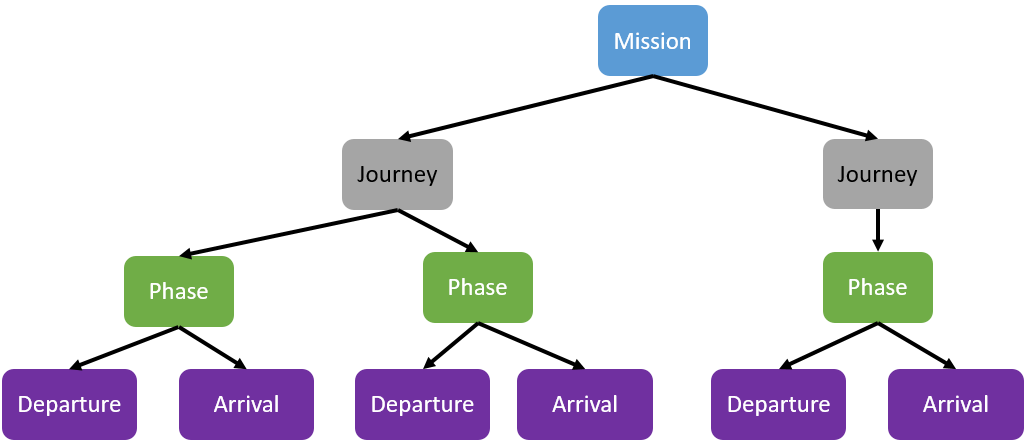
\includegraphics[width=0.9\linewidth]{EMTG_architecture_diagram.PNG}
	\caption{\label{fig:mission_architecture} Architecture of an \ac{EMTG} mission.}
\end{figure}

The \texttt{Mission} class has the following methods:

\begin{itemize}
	\item \texttt{calcbounds()} - Calculates the upper and lower bounds, as well as scale factors, for any owned decision variables and constraints. Calls the \texttt{calcbounds()} methods of any owned \texttt{Journey} and \texttt{ObjectiveFunction} objects.
	\item \texttt{evaluate()} - Evaluates any owned constraints and their partial derivatives. Calls the \texttt{evaluate()} methods of any owned \texttt{Journey} and \texttt{ObjectiveFunction} objects.
	\item \texttt{output()} - Writes the .emtg output file for the evaluated mission. Calls the \texttt{output()} methods of any owned \texttt{Journey} and \texttt{ObjectiveFunction} objects. Writes the mission-end summary, including all propellant and dry mass information for all spacecraft stages, plus the final decision vector and constraint vector.
	\item \texttt{output\_ephemeris()} - Writes an ephemeris file and acceleration output file for the evaluated mission by calling the \texttt{output\_ephemeris()} of any owned \texttt{Journey} objects. Writes a .cmd and .py file that uses \texttt{mkspk.exe} to create a SPICE kernel from the ephemeris file.
	\item \texttt{output\_STMs()} - Writes text files for each state transition matrix (STM) in the mission by calling the \texttt{output\_STMs()} method on any owned \texttt{Journey} objects.
	\item \texttt{output\_maneuver\_and\_target\_spec()} - Writes maneuver and target specification files by calling the \texttt{output\_maneuver\_and\_target\_spec()} methods of any owned \texttt{Journey} objects. These files are read by PIRATE, MONSTER, PyGMATscripter, and eventually also interfaces to Monte and provide the necessary information to re-target each maneuver in an operational navigation tool.
	\item \texttt{construct\_initial\_guess()} - Constructs the initial guess for the optimization problem. The user-provided \texttt{trialX} field in the \texttt{missionoptions} structure is compared to the mission \texttt{Xdescriptions} vector via string matching. Values from \texttt{trialX} are inserted into the initial guess vector when their descriptions match. If state representations do not match, \textit{i.e.} if the user has specified an initial guess in \texttt{SphericalRADEC} coordinates but the \texttt{missionoptions} file is configured to use \texttt{SphericalAZFPA} coordinates, then the user is warned. Low thrust phase initial guesses, whether they be based on two-point shooting or parallel shooting transcriptions, are interpolated to the number of time segments and interior control points requested by the user for that phase. Once all initial guess values are assigned, they are clipped to remain inside the \texttt{Xupperbounds} and \texttt{Xlowerbounds} vectors that were generated by the constructor. Finally, if any values remain unspecified, \texttt{construct\_initial\_guess} populates the with random values between the allowed bounds.
	\item \texttt{getUnscaledObjective()} - Returns the unscaled value of the objective function.
	\item \texttt{getJourney()} - Returns a pointer to the desired \texttt{Journey} object.
\end{itemize}

In addition, because \texttt{Mission} is \textit{not} derived from \texttt{sparsey\_thing}, \texttt{Mission} also implements the following utility methods:

\begin{enumerate}
	\item \texttt{create\_sparsity\_entry()}
	\item \texttt{create\_sparsity\_vector()}
\end{enumerate}

\section{Mission Time Constraint}
\label{sec:mission_time_constraint}

The user may impose constraint on total mission flight time. This is simply the sum of all of the time variables in the mission. \ac{EMTG} locates these by iterating through the \texttt{Xdescriptions} vector and adding up all decision variables that contain the string ``time.''

\section{Propellant and dry mass constraints}
\label{sec:propellant_and_dry_mass_constraints}

\texttt{Mission} may track constraints on chemical fuel, chemical oxidizer, electric, propellant, and/or dry mass. The user may choose to impose these globally, \textit{i.e.} over the entire mission, or at the spacecraft \texttt{stage} level.

All propellant usage in \ac{EMTG} is tracked by means of ``virtual tank'' variables. The nonlinear computations of true propellant use are book-kept as locally as possible in individual \texttt{Phase} and boundary event objects. Each maneuver is assigned a ``virtual tank'' variable and constraint. The ``virtual tank'' variable is a free parameter and is constrained to match the computed value of actual propellant use. The total amount of each type of propellant may then be computed by a linear sum of all of the associated virtual tank variables.

The \texttt{Spacecraft} object keeps track of the indices in the decision vector corresponding to the virtual tank variables for each propellant type. In addition, each individual \texttt{Stage} object keeps track of the indices corresponding to the virtual tank variables of each propellant type assigned to that stage. \texttt{Mission}'s only responsibility is to sum up all of the virtual tank variables for each global or stage propellant constraint. The lower bound on each propellant tank constraint is 0.0 kg and the upper bound is the user-defined size of the tank, adjusted by the user-defined propellant margin.

The global and stage dry mass constraints are computed by subtracting the total propellant consumed, plus user-defined margin, from the encoded final mass of the spacecraft. If the spacecraft either dropped mass (\textit{e.g.} dropped a probe) or added mass (\textit{e.g.} picked up a rock from an asteroid), then this mass is also accounted for.

Finally, the user may choose to constrain ``final mass'' instead of ``dry mass.'' This is just a constraint applied directly to the final state of the spacecraft, ignoring any propellant margin.

\chapter{Journey}
\label{chap:journey}

\section{Overview}
\label{sec:journey_overview}

The \texttt{Journey} class is an intermediate container that is a member of \texttt{Mission} and owns a \texttt{boost::ptr\_vector} of \texttt{Phase} objects. \texttt{Journey} inherits from \texttt{sparsey\_thing} and therefore contains pointers to all of the data vectors that define the \ac{NLP} problem and all of the utility methods that compute the Jacobian sparsity pattern.

The \texttt{Journey} class has the following methods:

\begin{itemize}
	\item \texttt{calcbounds()} - Calculates the upper and lower bounds, as well as scale factors, for any owned decision variables and constraints. Calls the \texttt{setup\_calcbounds()} and \texttt{calcbounds()} methods of any owned \texttt{Phase} objects.
	\item \texttt{process\_journey()} - Evaluates any owned constraints and their partial derivatives. Calls the \texttt{evaluate()} methods of any owned \texttt{Phase} objects.
	\item \texttt{output()} - Writes the .emtg output file for the evaluated journey. Calls the \texttt{output()} methods of any owned \texttt{Phase} objects. Writes the header for each journey, any mass increments, the boundary states, approximated ephemeris-pegged flyby periapse states, and any mass drops. Calls the \texttt{output\_specialized\_constraints()} method on the arrival and departure boundary events of each owned \texttt{Phase}.
	\item \texttt{output\_ephemeris()} - Writes an ephemeris file and acceleration output file for the evaluated mission by calling the \texttt{output\_ephemeris()} of any owned \texttt{Phase} objects. Writes a .cmd and .py file that uses \texttt{mkspk.exe} to create a SPICE kernel from the ephemeris file.
	\item \texttt{output\_STMs()} - Writes text files for each state transition matrix (STM) in the mission by calling the \texttt{output\_STMs()} method on any owned \texttt{Phase} objects.
	\item \texttt{output\_maneuver\_and\_target\_spec()} - Writes maneuver and target specification files by calling the \texttt{output\_maneuver\_and\_target\_spec()} methods of any owned \texttt{Phase} objects. These files are read by PIRATE, MONSTER, PyGMATscripter, and eventually also interfaces to Monte and provide the necessary information to re-target each maneuver in an operational navigation tool.
	\item \texttt{getNumberOfPhases()} - Returns the number of owned \texttt{Phase} objects.
	\item \texttt{getPhase()} - Returns a pointer to the desired \texttt{Phase} object.
	\item \texttt{getFirstPhase()} - Returns a pointer to the first \texttt{Phase} object.
	\item \texttt{getLastPhase()} - Returns a pointer to the last \texttt{Phase} object.
	\item \texttt{getDeterministicDeltav()} - Sums and returns the deterministic $\Delta v$ in the owned \texttt{Phase} objects. Each \texttt{Phase} is responsible for computing its deterministic $\Delta v$.
	\item \texttt{getStatisticalDeltav()} - Sums and returns the statistical $\Delta v$ in the owned \texttt{Phase} objects. Each \texttt{Phase} is responsible for computing its statistical $\Delta v$.
	\item \texttt{getFinalMass()} - Returns the mass at the end of the last \texttt{Phase} in this journey.
\end{itemize}


\section{Journey-end $\Delta v$}
\label{sec:journey_end_deltav}

The user may define a fixed \texttt{journey\_end\_deltav} for each \texttt{Journey}. This could represent, for example, a known set of maneuvers that will be performed after arrival at the target body. This could be expressed as a fixed mass drop, but \texttt{journey\_end\_deltav} allows the user to define a $\Delta v$ and apply it against the spacecraft mass at the end of the journey, using the appropriate spacecraft \texttt{Stage} monoprop system.

The actual computation of propellant use for the journey-end $Delta v$ is done in \texttt{ArrivalEvent}, but \texttt{Journey} extracts that information from the last \texttt{Phase} and outputs it.

\section{Journey time and epoch constraints}
\label{sec:journey_time_and_epoch_constraints}

The user may elect to constrain a given \texttt{Journey}'s departure date. This is done by summing the launch epoch and all of the flight time variables that occur prior to the beginning of the \texttt{Journey}.

In addition, the user may choose to constrain a \texttt{Journey}'s \textit{flight time}, \textit{aggregate flight time}, or \textit{arrival epoch}. It is not currently possible to constrain more than one of these at a time.

\textit{Flight time} refers to the sum of all phase time of flight variables and boundary event time widths in the \texttt{Journey}. \textit{Aggregate flight time} refers to the sum of all phase flight time and boundary event time width variables up to and including the \texttt{Journey}. \textit{Arrival epoch} computed by adding the launch epoch to the \textit{aggregate flight time}.

\externaldocument{../hardware_models/c-hardware_models}
\externaldocument{../astrodynamics/c-astrodynamics}
\externaldocument{../integration/c-integration}

\chapter{Phase}
\label{chap:phase}

\section{Phase base class}
\label{sec:phase_base_class}

\texttt{Phase} is the abstract base class from which all \ac{EMTG} phase types derive. The full phase class hierarchy is described in the EMTG Doxygen for the \texttt{phase} class. Every phase contains a \texttt{DepartureEvent} and an \texttt{ArrivalEvent} as described in Chapter \ref{chap:boundary-conditions}.

The base \texttt{Phase} class is also responsible for appropriately setting the stage of the spacecraft (Section \ref{sec:spacecraft}) based on user-defined values of \texttt{stage\_after\_departure}, \texttt{stage\_before\_arrival}, and \texttt{stage\_after\_arrival}.

\texttt{Phase} is responsible for calling the left and right boundaries' \texttt{calcbounds} and \texttt{process\_event} methods. \texttt{Phase} also computes the phase's initial TCM, if any, using the spacecraft's monoprop thrusters as described in Section \ref{subsec:ChemicalPropulsionSystem}.

When the phase is evaluated, \texttt{phase} calls \texttt{process\_event} on the departure and arrival events to determine the state of the spacecraft after departure and before arrival. Processing of everything that happens between the boundary points is handled by the derived phase classes as described later in this chapter.

\texttt{Phase} implements one, the time of flight ($TOF$) for the phase. The lower and upper bounds of the phase time of flight are determined based on the boundary events as described in \texttt{phase::calcbounds\_phase\_flight\_time()}.

\texttt{Phase} also implements one optional constraint. If \texttt{stage\_after\_departure} is set, then \texttt{phase} constrains the initial mass to be greater than or equal to the current stage dry mass as defined in the spacecraft definition file (Section \ref{sec:spacecraft}).

All phase classes in EMTG define the following methods:
\begin{itemize}
	\item \textbf{setup\_calcbounds()} - Sets up pointers to variable holders needed in the calcbounds process. Performs this task for not only the phase itself but also its owned departure and arrival boundary events.
	\item \textbf{calcbounds()} - Controls the calculation of bounds and sparsity pattern for the phase's decision variables and constraints by calling the below listed calcbounds methods.
	
	\item \textbf{calcbounds\_phase\_main()} - Calculates the bounds and sparsity pattern of variables and constraints defined by the derived phase class.
	
	\item \textbf{calcbounds\_virtual\_propellant\_tanks()} - Calculates the bounds and sparsity pattern of the phase's virtual propellant tank variables and constraints.
	
	\item \textbf{calcbounds\_deltav\_contribution()} - Calculates the bounds and sparsity pattern of the phase's contribution to the mission $\Delta v$. Only called when the minimum $\Delta v$ objective function is used.
	
	\item \textbf{process\_phase()} - Evaluates the phase's constraints and contribution to the objective function by calling the below listed process methods.

	\item \textbf{process\_phase\_main()} - Evaluates the phase transcription. This is always overriden by the derived class.
	
	\item \textbf{process\_phase\_left\_boundary()} - Calls the phase's departure event's process method and populates any data fields associated with the left-hand side of the phase. Handles the post-departure TCM if applicable. Handled by the base class.
	
	\item \textbf{process\_phase\_flight\_time()} - Computes the bounds on the phase time of flight. Usually handled by the base class but can be overriden for special phase types. Generally these phase types would still call the base class but then also define additional time-related variables.
	
	\item \textbf{process\_phase\_right\_boundary()} - Calls the phase's arrival event's process method and populates any data fields associated with the right-hand side of the phase. Handled by the base class.
	
	\item \textbf{process\_virtual\_propellant\_tanks()} - Computes the virtual propellant constraints, \textit{i.e.} requires that the actual propellant consumed match the virtual propellant.
	
	\item \textbf{process\_deltav\_contribution()} - Computes the phase's contribution to the total mission $\Delta v$.

	\item \textbf{output()} - Writes lines to the .emtg summary file.
	\item \textbf{output\_ephemeris()} - Writes lines to the .ephemeris file. This file may be configured to provide a high-resolution summary of systems parameters (mass, thrust, \ac{Isp}, \textit{etc.}) or may alternately be written out as just state and epoch and then used to make a SPICE kernel.
	\item \textbf{output\_maneuver\_and\_target\_spec()} - Writes lines to the .maneuver\_spec and .target\_spec files, which are used as an interface to flight-fidelity maneuver planning tools.
\end{itemize}

\section{TwoPointShootingPhase}
\label{sec:two_point_shooting_phase}

\texttt{TwoPointShootingPhase} is an abstract base class for all phase transcriptions that employ two point shooting. In other words, all phases where the spacecraft is propagated forward from the left-hand boundary condition and backward from the right-hand boundary condition. A set of match point constraints is employed to link the forward and backward half-phases together. The derivatives of the match point constraints with respect to the boundary variables may be computed via forward and backward \ac{HPTM}s, which in turn are constructed by chaining together all of the \ac{STM}s and \ac{MTM}s in the forward and backward half-phases.

\texttt{TwoPointShootingPhase} handles the creation of the match point constraints and the mapping of the partial derivatives of the boundary states to the match point constraints via the \ac{HPTM}s. Derivatives of the match point constraints with respect to variables internal to the phase, \textit{i.e.} control variables, are handled by the derived phase class.

\subsection{CoastPhase}
\label{subsec:CoastPhase}

\texttt{CoastPhase} is the simplest form of \texttt{TwoPointShootingPhase} in which the spacecraft travels from the left boundary to the right boundary without performing any maneuvers. The user may elect to propagate the trajectory via a Kepler propagator or via numerical integration with a higher-fidelity force model. In both cases, the propagation is done in the time domain.

If a numerical integrator is used, the user may independently control the step size on either side of the match point. The user specifies a time step size in seconds for the first (\texttt{CoastPhaseForward-\\IntegrationStepLength}) and second (\texttt{CoastPhaseBackwardIntegrationStepLength}) half-phase. The user may also choose \texttt{CoastPhaseMatchPointFraction} in $\left[0, 1\right]$, the fixed fraction of the phase flight time at which the match point occurs. The default value is 0.5, corresponding to a match point exactly halfway through the phase. A lower number moves the match point closer to the left-hand boundary and a higher number moves the match point closer to the right-hand boundary.

\texttt{CoastPhase} adds no new variables or constraints to the problem.

\subsection{SundmanCoastPhase}
\label{subsec:sundmancoastphase}

\texttt{SundmanCoastPhase} is identical to \texttt{CoastPhase} except that it uses a Sundman propagator instead of a time-domain propagator. An additional decision variable is added to represent the Sundman anomaly traversed over the course of the phase, and an epoch continuity constraint is added at the match point. \texttt{SundmanCoastPhase} is designed for high-fidelity modeling of gravity assists without requiring tight time steps.

\texttt{SundmanCoastPhase} is implemented in EMTGv9 with an integrated propagator and provides full analytical derivatives. The independent variable is a scaled Sundman anomaly that roughly corresponds to eccentric anomaly. EMTGv9 does not yet have a Keplerian Sundman propagator, and so SundmanCoastPhase will not work in Kepler mode. But, since Kepler mode is so fast anyway, you wouldn't want to do that.

\subsection{MGAnDSMs}
\label{subsec:MGAnDSMs}

\ac{EMTG}'s Multiple Gravity Assist with \textit{n} Deep-Space Maneuvers (\texttt{MGAnDSMs}) transcription models the flight of a spacecraft using high-thrust chemical propulsion. The maneuvers are encoded as impulsive events, \textit{i.e.} they happen instantaneously, and the optimizer may place maneuvers in any permitted location in the phase. The user chooses the maximum number of impulses \textit{a priori}. If the specified number of impulses is more than what is needed, the optimizer will reduce the magnitude of any un-needed maneuvers to zero. \texttt{MGAnDSMs} derives from \texttt{TwoPointShootingPhase}.

The trajectory is propagated forward in time from the left-hand boundary condition and backward in time from the right-hand boundary condition. The optimizer chooses the time of flight ($TOF$) for the phase, along with necessary parameters to define the magnitude and direction of any impulsive \ac{DSM}s. The $TOF$ from the left-hand boundary to the first \ac{DSM}, as well as from each \ac{DSM} to the next \ac{DSM} or to the right-hand boundary where appropriate, is expressed as the product of a ``burn index'' $\eta_i$ with the phase $TOF$. The sum of the $\eta_i$ must equal 1.0, guaranteeing that the propagation arcs fit within the phase $TOF$. Therefore, if a phase has only one impulse, then the time from the left boundary to the \ac{DSM}, $\Delta t_1$, and the time from the DSM to the right boundary, $\Delta t_2$ will be:

\begin{align}
\Delta t_1 &= \eta_1 TOF\\
\Delta t_2 &= \eta_2 TOF
\label{eq:MGAnDSMs_time_calculations}
\end{align}

Mass is propagated across each impulse by means of the exponential form of the rocket equation as shown in Equation \ref{eq:rocket_equation}.

\begin{equation}
m_i^+ = m_i^- \exp \left(\frac{-\Delta v}{I_{sp} g_0}\right)
\label{eq:rocket_equation}
\end{equation}
%
where $m_i^-$ is the mass of the spacecraft before the maneuver, $m_i^+$ is the mass of the spacecraft after the maneuver, $\Delta v$ is the magnitude of the impulsive \ac{DSM}, $g_0$ is the acceleration due to gravity at sea level on Earth, and $I_{sp}$ is the specific impulse of the spacecraft's thruster. A constant mass leak term may be used to approximate propellant consumption due to \ac{ACS} desat maneuvers. \ac{EMTG} keeps track of fuel and oxidizer consumption separately so that they may be individually constrained.

The decision variables and constraints necessary to define an \ac{MGAnDSMs} phase are listed in Tables \ref{tab:decision_variables_MGAnDSMs} and \ref{tab:constraints_MGAnDSMs}, respectively. A diagram of the \ac{MGAnDSMs} phase architecture is shown in Figure \ref{fig:MGAnDSMs}. The subscript $_{mp}$ denotes that a given constraint is expressed at the match point.

\begin{figure}
	\centering
	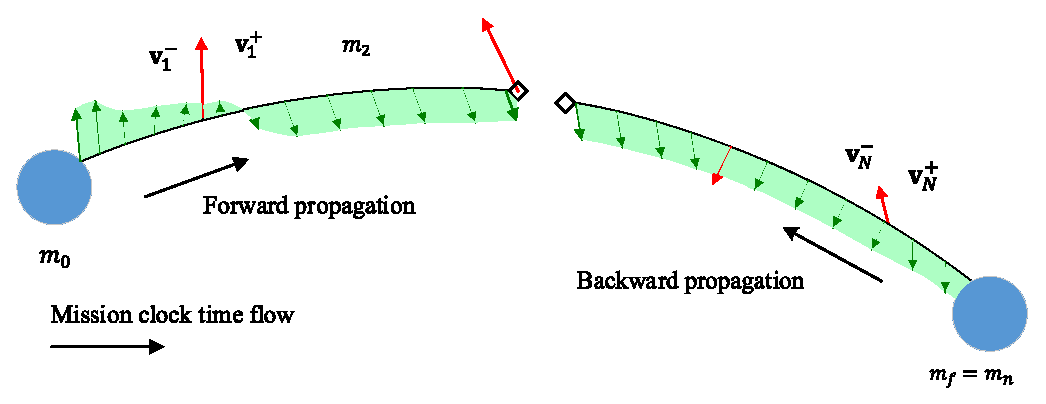
\includegraphics[width=0.8\linewidth]{./mission/MGAnDSMsphase_no_legend.eps}
	\caption{\label{fig:MGAnDSMs} Diagram of the \ac{MGAnDSMs} transcription. The red arrows represent impulsive \ac{DSM}s, and the green-highlighted black arrows represent natural perturbations.}
\end{figure}

\begin{table}
	\centering
	\caption{Unique variables that define an \ac{MGAnDSMs} phase}
	\label{tab:decision_variables_MGAnDSMs}
	\begin{tabular}{ll}
		\hline\hline
		Variable & Description\\
		\hline
		$\eta_i$ &Fractions of the phase $TOF$ that define the time between \ac{DSM}s and the\\
		& boundaries, as well as between \ac{DSM}s and other \ac{DSM}s. One per \ac{DSM}\\
		& plus one for the right-hand boundary.\\
		$\Delta v_{i,x}$ & $x$ component of \ac{DSM} $i$. One per \ac{DSM}\\
		$\Delta v_{i,y}$ & $y$ component of \ac{DSM} $i$. One per \ac{DSM}\\
		$\Delta v_{i,z}$ & $z$ component of \ac{DSM} $i$. One per \ac{DSM}\\
		$m_{fuel-virtual}$ & virtual chemical fuel tank\\
		$m_{ox-virtual}$ & virtual chemical oxidizer tank\\
		\hline\hline		
	\end{tabular}
\end{table}

\begin{table}
	\centering
	\caption{Constraints that define an \ac{MGAnDSMs} phase.}
	\label{tab:constraints_MGAnDSMs}
	\begin{tabular}{ll}
		\hline\hline
		Constraint & Depends on\\
		\hline		
		$x^+_{mp} = x^-_{mp}$& $TOF$, all $\eta_i$, all $\Delta v_{i,x}$, all $\Delta v_{i,y}$, all $\Delta v_{i,z}$, boundary variables\\
		$y^+_{mp} = y^-_{mp}$& $TOF$, all $\eta_i$, all $\Delta v_{i,x}$, all $\Delta v_{i,y}$, all $\Delta v_{i,z}$, boundary variables\\
		$z^+_{mp} = z^-_{mp}$& $TOF$, all $\eta_i$, all $\Delta v_{i,x}$, all $\Delta v_{i,y}$, all $\Delta v_{i,z}$, boundary variables\\
		$\dot{x}^+_{mp} = \dot{x}^-_{mp}$& $TOF$, all $\eta_i$, all $\Delta v_{i,x}$, all $\Delta v_{i,y}$, all $\Delta v_{i,z}$, boundary variables\\
		$\dot{y}^+_{mp} = \dot{y}^-_{mp}$& $TOF$, all $\eta_i$, all $\Delta v_{i,x}$, all $\Delta v_{i,y}$, all $\Delta v_{i,z}$, boundary variables\\
		$\dot{z}^+_{mp} = \dot{z}^-_{mp}$& $TOF$, all $\eta_i$, all $\Delta v_{i,x}$, all $\Delta v_{i,y}$, all $\Delta v_{i,z}$, boundary variables\\
		$m^+_{mp} = m^-_{mp}$& $TOF$, all $\eta_i$, all $\Delta v_{i,x}$, all $\Delta v_{i,y}$, all $\Delta v_{i,z}$, boundary variables\\
		$m^+_{fuel-mp} = m^-_{fuel-mp}$& $TOF$, all $\eta_i$, all $\Delta v_{i,x}$, all $\Delta v_{i,y}$, all $\Delta v_{i,z}$, boundary variables\\
		$m^+_{ox-mp} = m^-_{ox-mp}$& $TOF$, all $\eta_i$, all $\Delta v_{i,x}$, all $\Delta v_{i,y}$, all $\Delta v_{i,z}$, boundary variables\\
		$\sum_{i=1}^{n+1} \eta_i = 1.0$ & all $\eta_i$\\
		\hline\hline		
	\end{tabular}
\end{table}

Each impulse/propagate pair in a \texttt{MGAnDSMs} phase is called a \texttt{MGAnDSMs\_subphase}. \texttt{MGAnDSMs\_subphase} is also the named of an abstract base class with two derived classes, \texttt{Forward\_MGAnDSMs\_subphase} and \texttt{Backward\_MGAnDSMs\_subphase}. These two derived classes handle the actual computation of the maneuvers and propagation of the trajectory in the forward and backward sides of the phase, respectively. The parent \texttt{MGAnDSMs} owns vectors of \texttt{Forward\_MGAnDSMs\_subphase} and \texttt{Backward\_MGAnDSMs\_subphase} objects, and is responsible for assembling the half-phase transition matrices by chaining the individual subphase state transition matrices.

\subsubsection{MGAnDSMs maneuver constraints}
\label{subsubsec:MGAnDSMs_maneuver_constraints}

Each \texttt{MGAnDSMs\_subphase} contains a vector of \texttt{MGAnDSMs\_maneuver\_constraint} objects. \texttt{MGAnDSMs\_maneuver\_constraint} is an abstract base class from which a wide variety of constraints are derived. Their uses are described in the scripted constraints document. Currently we can constrain maneuver magnitude and epoch both in an absolute sense and relative to other epochs in the phase.

\texttt{MGAnDSMs\_maneuver\_constraint} objects are constructed by the \texttt{MGAnDSMs\_maneuver\_constraint\_factory}. Whenever a developer adds a new constraint, the factory must be updated.

\subsection{TwoPointShootingLowThrustPhase}
\label{subsec:TwoPointShootingLowThrustPhase}

\texttt{TwoPointShootingLowThrustPhase} is an abstract base class that is derived from \texttt{TwoPointShootingPhase}. \texttt{TwoPointShootingLowThrustPhase} is a base class for all transcriptions that model a spacecraft operating with continuous thrust (often low-thrust) propulsion for the entire phase. The user may impose forced initial and/or terminal coasts of fixed duration at the beginning and end of the phase, respectively.

Any remaining flight time not consumed by the forced coasts is available for thrusting. The thrust time is divided up into an even number of control segments, with an equal number of segments on either side of the match point. The segments are assigned equal length in the independent variable of integration. This is usually time but it is possible to construct a derived phase type that integrates over true anomaly or mean anomaly instead of time.

A control 3-vector $\mathbf{u}$ is applied at each control segment. There are 3\textit{n} control variables in a TwoPointShootingLowThrustPhase, where \textit{n} is the number of control segments. The magnitude of $\mathbf{u}$ represents the commanded duty cycle for the control segment, and is constrained to not exceed 1.0. The user may elect to force the control to have unit magnitude for all control segments, in which case the lower bound is also 1.0, or to force the control to have zero magnitude, in which case the lower and upper bounds are both 0.0. \hl{Previous versions of EMTG allowed for a fourth control variable at each step, $u_{command}$. $u_{command}$ was used to control properties of the propulsion system, such as input voltage or mass flow rate. \texttt{TwoPointShootingLowThrustPhase} does not currently support $u_{command}$ but the design allows for it to be added at a later date. The STMs and MTMs would just need an additional row and column.} The user may also elect to force the all of the control vectors in a phase to match each other, creating a fixed inertial pointing phase.

\texttt{TwoPointShootingLowThrustPhase} also implements two virtual propellant tank variables. One always represents chemical fuel, whether for main propulsion or for \ac{ACS} desats. The other represents electric propellant. These virtual tank variables may be added together to compute a linear constraint on propellant consumption across all phases and boundary events in the mission. Constraints are added to ensure that the virtual propellant variables match the actual propellant consumed in the phase. The latter is highly nonlinear and is handled with extra rows and columns in the \ac{STM} and \ac{MTM} in each derived phase class.

\hl{As of this writing, EMTG assumes that the spacecraft has single-axis articulated solar arrays. This is important because there is therefore no dependence of available power on thrust direction. Fixed arrays would have cosine losses, which are not yet modeled.}

\subsubsection{MGALT}
\label{subsubsec:MGALT}

\texttt{MGALTphase} is a low-fidelity transcription for continuous-thrust (often low-thrust) phases. It derives from \texttt{TwoPointShootingLowThrustPhase} and models the trajectory using the Sims-Flanagan transcription. The low-thrust perturbation is approximated across each control segment by a bounded impulse, where the magnitude of the impulse is equal to the maximum $\Delta v$ that could be accomplished by thrusting continuously across the thrust segment. The spacecraft is propagated between impulses by solving Kepler's equation.

The full mathematical details of the \ac{MGALT} transcription are provided in References \cite{BoundedImpulseDerivatives1} and \cite{BoundedImpulseDerivatives2}. This section discusses only the software architecture.

The calculations of available power, thrust, and mass flow rate are performed by the spacecraft model and the \texttt{BoundedImpulseManeuver} abstract base class. The mathematics of each forward or backward thrust-and-propagation step are performed by the derived \texttt{ForwardBoundedImpulseManeuver} and \texttt{BackwardBoundedImpulseManeuver} classes, respectively. The computation of derivatives is slightly different between the forward and backward versions and so two classes are necessary.

\texttt{ForwardBoundedImpulseManeuver} and \texttt{BackwardBoundedImpulseManeuver} track not only the position, velocity, and mass of the spacecraft but also the propellant state. A constant mass leak term may be used to approximate propellant consumption due to \ac{ACS} desat maneuvers. \ac{ACS} propellant is applied against the spacecraft's ``chemical fuel'' tank, whereas main propulsion is applied against the ``electric propellant'' tank.

\texttt{MGALTphase} is responsible for holding data structures, a vector of \texttt{ForwardBoundedImpulseManeuver} and \texttt{BackwardBoundedImpulseManeuver} calculation objects, and for assembling the forward and backward \ac{HPTM}s by chaining the \ac{STM}s and \ac{MTM}s as described in References \cite{BoundedImpulseDerivatives1} and \cite{BoundedImpulseDerivatives2}. \texttt{MGALTphase} also performs all file output.

The user may choose to constrain the distance between the spacecraft and any reference body at the center of each control segment. This computation is handled by the parent \texttt{MGALTphase} class. While effective, this set of constraints significantly slows the optimization process because computing the derivatives of the distance constraints with respect to the phase control variables produces a very dense sparsity pattern and requires many matrix multiplies.

\subsubsection{FBLT}
\label{subsubsec:FBLT}

\ac{FBLT} is identical to \ac{MGALT} in every way except that instead of the Sims-Flanagan transcription, \ac{FBLT} uses explicit numerical integration to propagate the equations of motion with a thrust perturbation supplied by the electric propulsion and power system models (Chapter \ref{chap:hardware_models}). Natural perturbations may also be added as described in Section \ref{sec:acceleration_model}.

\texttt{FBLTphase} derives from \texttt{TwoPointShootingLowThrustPhase} and adds no new decision variables or constraints. The user may elect to constrain the distance between the spacecraft and a reference body, as described in the scripted constraints document. As in \ac{MGALT}, the sparsity pattern of the distance constraint is a triangle and requires many \ac{STM} multiplications, and so the distance constraint adds significantly to the computation time necessary to optimize the mission.

\subsection{MGALTS}
\label{subsec:MGALTS}

\ac{MGALTS} is not yet implemented, but Donald and Jacob built a demonstrator once and will some day put it into EMTGv9 if anyone can figure out a use for it. It is just MGALT with a Sundman propagator, an additional decision variable for the Sundman anomaly traversed by the phase, and an epoch continuity constraint.

MGALTS uses a Keplerian Sundman propagator that is not yet implemented. Again, we'll build this if and when someone needs it. We did this in EMTGv8 and it worked but was not terribly useful. This subsection is a placeholder for now.

\subsection{FBLTS}
\label{subsec:FBLTS}

\ac{FBLTS} is not yet implemented, but Donald and Jacob built a demonstrator once and will some day put it into EMTGv9 if anyone can figure out a use for it. It is just FBLT with a Sundman propagator, an additional decision variable for the Sundman anomaly traversed by the phase, and an epoch continuity constraint.

FBLTS uses an integrated Sundman propagator. Again, we'll build this if and when someone needs it. We did this in EMTGv8 and it worked but was not terribly useful. This subsection is a placeholder for now.

\section{Parallel shooting phase classes}
\label{sec:parallel_shooting_phase}


\texttt{ParallelShootingPhase} is an abstract base class for phase transcriptions that model the path of a spacecraft using low-thrust propulsion via the method of direct parallel shooting \cite{enright1992}. In this technique, the phase is decomposed into a set of short shooting steps. The state vector is encoded as decision variables on the left-hand side of each short step and then propagated to the right-hand side. A set of nonlinear match point constraints are used to ensure that in a converged solution, the propagated right-hand side of the $(i-1)^{th}$ step matches the encoded left-hand side of the $i^{th}$ step. The constraints are encoded on the left-hand side of the $i^{th}$ step. The technique is called ``parallel shooting'' because all of the steps propagate in the same direction, \textit{i.e.} forward in time.

The primary role of \texttt{ParallelShootingPhase} is to hold a polymorphic vector of \texttt{ParallelShootingStep}-derived objects as described in the next paragraph. In addition, \texttt{ParallelSootingPhase} handles the forced initial and/or terminal coast if the user requests them. The terminal coast is backward propagated, unlike everything else in \texttt{ParallelShootingPhase}.

\texttt{ParallelShootingStep} is the abstract base class for a propagation step in \texttt{ParallelShootingPhase}. It handles the encoding of the left-hand side state vector and the match point constraints that connect to the right-hand side of the previous step. As of this writing, \texttt{ParallelShootingStep} can encode the state vector in \texttt{SphericalRADEC} or \texttt{SphericalAZFPA} coordinates. The match point constraints are always encoded in cartesian coordinates. \hl{Additional state and constraint representations can easily be added.} The phase type-specific derived classes of \texttt{ParallelShootingStep} are also responsible for mapping the partial derivatives of the left-hand state to the right-hand state by means of \ac{STM}s and \ac{MTM}s that are unique to that phase type. In addition to position and velocity, \texttt{ParallelShootingStep} also encodes decision variables and continuity constraints for spacecraft mass, virtual chemical fuel mass, and virtual electric propellant mass.

There are three abstract base classes that themselves derive from \texttt{ParallelShootingStep}. \texttt{ParallelShootingFirstStep} is the abstract base class for the first step in a \texttt{ParallelShootingPhase}. It is unique in that instead of retrieving right-hand propagated state information from the previous step, it pulls the state after the initial coast from the parent \texttt{ParallelShootingPhase}. \texttt{ParallelShootingLastStep} is the abstract base class for the last step in a \texttt{ParallelShootingPhase} and is unique because it has two sets of match point constraints - the usual one on the left-hand side and another set on the right-hand side to ensure that the propagated right-hand state matches the \texttt{ParallelShootingPhase}'s state prior to the terminal coast. Finally, \texttt{ParallelShootingOneStepToRuleThemAll} is an abstract base class for the special case where a \texttt{ParallelShootingPhase} has only one step and has the properties of both \texttt{ParallelShootingFirstStep} and \texttt{ParallelShootingLastStep}.

\subsection{PSFB}
\label{subsec:PSFB}

\ac{PSFB} is a transcription for modeling the path of a low-thrust spacecraft using direct parallel shooting and a high-fidelity model of both the natural and spacecraft dynamics. \ac{PSFB} consists of the \texttt{PSFBphase}, \texttt{PSFBstep}, \texttt{PSFBfirststep}, \texttt{PSFBlaststep}, and \texttt{PSFBOneStepToRuleThemAll} classes that are each derived from the corresponding base class in Section \ref{sec:parallel_shooting_phase}, as well as a \texttt{PSFBstep\_factory} that creates the various types of step.

\ac{PSFB} propagates the trajectory using explicit numerical integration as described in Chapter \ref{chap:integration} and \ac{EMTG}'s full dynamics and spacecraft model as described in Chapters \ref{chap:astrodynamics} and \ref{chap:hardware_models}. Just as in \ac{EMTG}'s other transcriptions, control is piecewise constant across a segment. The user selects to have one \textit{or more} control opportunities per segment. If more than one control opportunity is chosen then the segment is broken into equal-length control steps. Control is encoded as a 3-vector just as in \ac{MGALT} and \ac{FBLT}. \hl{There is currently no provision for a fourth control variable but it would not be too difficult to add one.} The user may elect to force the all of the control vectors in a phase to match each other, creating a fixed inertial pointing phase. The user may also elect to force the control to be either full on or full off across the phase. Figure \ref{fig:PSFB} shows a \ac{PSFB} phase.

The \ac{PSFB} derived classes are responsible only for propagation, calculation of \ac{STM}s, and output. All of the book-keeping is handled by the base classes.

\begin{figure}
	\centering
	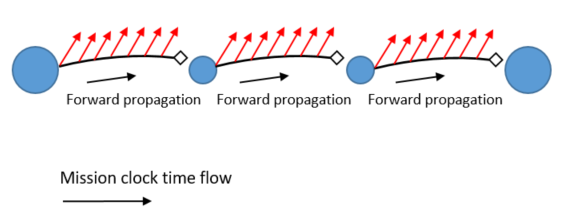
\includegraphics[width=0.8\linewidth]{./mission/PSFB.png}
	\caption{\label{fig:PSFB} Diagram of the \ac{PSFB} transcription. The red arrows represent a continuous thrust perturbation.}
\end{figure}

\FloatBarrier

\subsubsection{PSFB with high-fidelity duty cycle}
\label{subsubsec:PSFB_with_high_fidelity_duty_cycle}

\ac{PSFB}, like \ac{FBLT}, models propulsion duty cycle by multiplying the maximum duty cycle by the commanded thrust and mass flow rate. While this averaged duty cycle is sufficient for trade studies and sensitivity analysis, it may not always be acceptable as an initial guess for a flight-fidelity maneuver planning tool. \ac{EMTG} provides an alternative form of the \ac{PSFB} transcription that explicitly models the individual thrust arc and the short coast that exist in each thrust segment. The coast period is set aside for tracking, communication, other mission needs (\textit{e.g.} optical navigation), and contingencies. As with all of \ac{EMTG}'s other low-thrust transcriptions, power and propulsion characteristics are continuously evaluated as the trajectory is propagated and so thruster mode transitions can occur during a segment. Figure \ref{fig:PSFB_hifi_duty} shows three \ac{PSFB} steps with high-fidelity duty cycle modeling and thrust transitions due to a high-fidelity propulsion model.

\begin{figure}
	\centering
	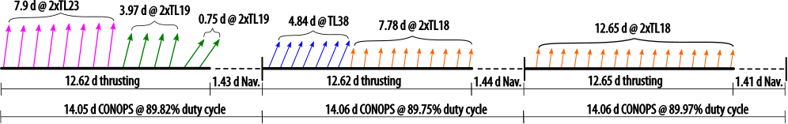
\includegraphics[width=0.8\linewidth]{./mission/PSFB_hifi_duty_cycle.png}
	\caption{\label{fig:PSFB_hifi_duty} Diagram of a three \ac{PSFB} steps with high-fidelity duty cycle modeling.}
\end{figure}

The high-fidelity duty cycle variant of \ac{PSFB} is implemented by creating yet another set of derived classes: \texttt{PSFB\_HifiDuty\_step}, \texttt{PSFB\_HifiDuty\_firststep}, \texttt{PSFB\_HifiDuty\_laststep}, and \texttt{PSFB\_HifiDuty\_OneStepToRuleTHemAll}. No new phase class is necessary because the container of \texttt{PSFBstep} objects in \texttt{PSFBphase} is polymorphic and can be populated with the high-fidelity duty cycle variants instead.

\subsection{PSBI}
\label{subsec:PSBI}

\acl{PSBI} (\acs{PSBI}) is a low-fidelity parallel-shooting transcription that combines the Sims-Flanagan model \cite{SimsFlanagan1999} with the base parallel-shooting phase classes. In \ac{PSBI}, the low-thrust acceleration is modeled as a bounded impulse in the center of each time step just as in \ac{MGALT}. Just as in \ac{PSFB}, each time-step encodes its left-hand state in the decision vector and includes a set of continuity constraints to ensure that the encoded left-hand state matches the previous step's propagated right-hand state. Figure \ref{fig:PSBI_diagram} describes the \ac{PSBI} transcription.

\begin{figure}[hb]
	\centering
	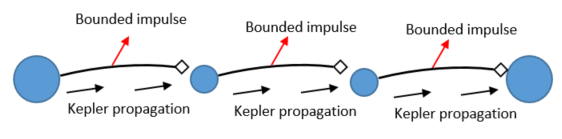
\includegraphics[width=0.8\linewidth]{./mission/PSBI.png}
	\caption{ The \ac{PSBI} transcription.}
	\label{fig:PSBI_diagram}
\end{figure}

\ac{PSBI} is composed of the \texttt{PSBIphase} container class, the \texttt{PSBIstep} base class for time steps, and the \texttt{PSBIfirststep}, \texttt{PSBIlaststep}, and \texttt{PSBIOneStepToRuleThemAll}. Each of these is derived from the corresponding abstract base class for \texttt{ParallelShootingPhase} as described in Section \ref{sec:parallel_shooting_phase}. The \ac{PSBI} step classes are constructed by \texttt{PSBIstep\_factory}.

\ac{PSBI} uses exactly the same decision variables and constraints as \ac{PSFB}, as defined in the base \texttt{ParallelShootingPhase} and child classes. Since \ac{PSBI} runs much faster than \ac{PSFB}, this enables the user to quickly converged a solution in \ac{PSBI} and then use it as an initial guess for \ac{PSFB}.

\subsection{Parallel Shooting Constraints}
\label{subsec:parallel_shooting_constraints}

The base \texttt{ParallelShootingStep} class contains vectors of \texttt{ParallelShootingStepDistanceConstraint} and \texttt{ParallelShootingStep\_maneuver\_constraint} objects. These constraints are enforced on the left-hand side of each segment. \texttt{ParallelShootingStepDistanceConstraint} is a stand-alone class that there is no need to inherit from as far as we can think of. Its use is described in the scripted constraints document.

\texttt{ParallelShootingStep\_maneuver\_constraint} is an abstract base class that is designed so that a developer may easily write derived classes to constraint maneuver magnitude, direction, etc. As of this writing (12/27/2019), there is only one such derived constraint, the Body-Probe-Thrust (BPT) angle constraint. This constraint is described in detail in the scripted constraints document. Maneuver constraints are the primary reason to use \ac{PSFB} and \ac{PSBI} instead of \ac{FBLT} and \ac{MGALT}. Maneuver constraints are very difficult to pose in a two-point shooting transcription but very easy in a parallel shooting transcription because the state vector at the left-hand side of each segment is encoded into the decision vector and no chaining is necessary.

\texttt{ParallelShootingStep\_maneuver\_constraint} objects are constructed by the \texttt{ParallelShootingStep\_maneuver\_constraint\_factory}.
	
\endinput

\externaldocument{../SplineEphem/c-SplineEphem}
\externaldocument{../hardware_models/c-hardware_models}

\chapter{Boundary Conditions}
\label{chap:boundary-conditions}

\section{BoundaryEventBase}
\label{sec:boundaryeventbase}

\texttt{BoundaryEventBase} is the abstract base class from which all boundary events are derived. The base class defines the interfaces common to all boundary events and also the common fields, including the state before and after the event. For a full class hierarchy of all boundary conditions, see ``EMTG::BoundaryEvents::BoundaryEventBase'' in the \ac{EMTG} Doxygen. All classes are described conceptually below.

\section{EdelbaumSpiral}
\label{sec:EdelbaumSpiral}

\texttt{EdelbaumSpiral} is an owned subclass of \texttt{EphemerisPeggedSpiralDeparture} and \texttt{EphemerisPeggedSpiralArrival} and handles the mathematics of a segmented Edelbaum Spiral. This technique is used in EMTG to approximate a many-revolution low-thrust spiral about a body in the current universe. For example, one may wish to spiral from LEO to escape from the Earth, or from the edge of the Mars sphere of influence down to the orbital distance of Phobos or Deimos. Edelbaum's approximation provides a fast, sufficiently accurate model that allows spirals to be included with an EMTG broad search without having to explicitly model and optimize the path of the spacecraft during the spiral.

Edelbaum's approximation consists of modeling the initial and final orbits about the body as co-planar circles and then assuming that the thrust level is sufficiently low that the transfer orbit is also nearly circular. The total $\Delta v$ for the transfer may then be written as:

\begin{equation}
	\label{eq:edelbaum_delta_v}
	\Delta v = \abs{\sqrt{\frac{\mu}{r_1} -\sqrt{\frac{\mu}{r_2}}}}
\end{equation}

Edelbaum's technique makes the assumption of constant thrust and specific impulse across the entire spiral. This does not accurately reflect a spiral using solar-electric propulsion about a body whose orbit has significant eccentricity because as the body moves closer to or farther from the sun, the available power changes and so does the available thrust and specific impulse. Accordingly, EMTG supports splitting an Edelbaum spiral into multiple segments, each modeling an equal portion of the spiral $\Delta v$. At the beginning of each segment, the power, thrust, and specific impulse are re-computed based on the body's distance from the sun.

The actual mathematics of the Edelbaum segments are handled in \texttt{EdelbaumSpiralSegment}. \texttt{EdelbaumSpiral} contains a vector of \texttt{EdelbaumSpiral} objects. Other than holding the segment objects, \texttt{EdelbaumSpiral}'s job is to calculate the total $\Delta v$ as per Equation \ref{eq:edelbaum_delta_v} and to provide the final state, \textit{i.e.} the state at the end of the final \texttt{EdelbaumSpiralSegment}, and its derivatives to the parent boundary condition object. \texttt{EdelbaumSpiral} does not itself introduce any new decision variables or constraints.

\subsection{EdelbaumSpiralSegment}
\label{subsec:EdelbaumSpiralSegment}

\texttt{EdelbaumSpiralSegment} is an owned subclass of \textit{EdelbaumSpiral} that performs the actual Edelbaum spiral calculations for each segment. The segment $\Delta v$ is provided at problem setup via Equation \ref{eq:edelbaum_delta_v} and is fixed during problem execution. In order to simplify the partial derivatives of the spiral's final state with respect to the decision variables, EMTG uses a ``sparse'' spiral transcription.

The time of flight, the mass at the end of the segment, and the electric propellant and chemical fuel (for ACS) consumed during the segment are encoded as decision variables as described in Table \ref{tab:decision_variables_EdelbaumSpiralSegment}. Nonlinear constraints are then imposed as per Table \ref{tab:constraints_EdelbaumSpiralSegment} to ensure that the encoded flight time, mass, and propellant match the computed flight time, mass, and propellant. These constraints are simple to formulate and have simple partial derivatives. EMTG can then compute the total propellant and time required for the spiral by simply adding up the relevant decision variables for each \texttt{EdelbaumSpiralSegment}.

\begin{table}
	\centering
	\caption{Decision variables that define an \texttt{EdelbaumSpiralSegment}}
	\label{tab:decision_variables_EdelbaumSpiralSegment}
	\begin{tabular}{ll}
		\hline\hline
		Variable & Description\\
		\hline
		$TOF$ & time-of-flight of the segment\\
		$m_f$ &mass at the right-hand side of the segment\\
		$m_{ep}$ & virtual electric propellant\\
		$m_{cf}$ &virtual chemical fuel (for ACS desats)\\
		\hline\hline		
	\end{tabular}
\end{table}

\begin{table}
	\centering
	\caption{Constraints that define an \texttt{EdelbaumSpiralSegment}}
	\label{tab:constraints_EdelbaumSpiralSegment}
	\begin{tabular}{ll}
		\hline\hline
		Constraint & Depends on\\
		\hline		
		$TOF_{computed} = TOF_{encoded}$& $TOF_{encoded}$, all previous time variables, $m_{i}$\\
		$m_{ep,computed} = m_{ep,encoded}$& $m_{ep,encoded}$, all previous time variables, $m_{i}$\\
		
		$m_{cf,computed} = m_{cf,encoded}$& $m_{cf,encoded}$, $m_{i}$ (if tracking ACS), $TOF_{encoded}$ (if tracking ACS)\\
		\hline\hline		
	\end{tabular}
\end{table}

The initial mass for each segment, $m_i$, is drawn either from the parent boundary condition's encoded mass (for the first segment) or from the previous segment's encoded final mass (for later segments).


\section{DepartureEvent}
\label{sec:departureevent}

\texttt{DepartureEvent} is an intermediate abstract base class that specializes \texttt{BoundaryEventBase} to the specific needs of a departure event. \texttt{DepartureEvent} is then an abstract base class for all of the various departure events described below.

The child departure events all derive both from \texttt{DepartureEvent} and from whatever class of boundary they are (\texttt{EphemerisPeggedboundary}, \texttt{EphemerisReferencedBoundary}, \texttt{FreePointBoundary}, or \texttt{PeriapseBoundary}).

Some departure events encode a ``wait time,'' \textit{i.e.} a decision variable that defines the period of time between either the \texttt{launch\_window\_open\_date} or the end of the previous journey, and the beginning of the current journey. The bounds on the wait time are defined by the user. Any departure event that has a wait time and begins a journey other than the first includes a mass continuity constraint such that the mass at the beginning of the departure event matches the mass at the end of the previous journey's arrival event.

\section{ArrivalEvent}
\label{sec:arrivalevent}

\texttt{ArrivalEvent} is an intermediate abstract base class that specializes \texttt{BoundaryEventBase} to the specific needs of a arrival event. \texttt{ArrivalEvent} is then an abstract base class for all of the various arrival events described below.

The child arrival events all derive both from \texttt{ArrivalEvent} and from whatever class of boundary they are (\texttt{EphemerisPeggedboundary}, \texttt{EphemerisReferencedBoundary}, \texttt{FreePointBoundary}, or \texttt{PeriapseBoundary}).

\clearpage
\section{EphemerisPeggedBoundary}
\label{sec:ephemerispeggedboundary}

\texttt{EphemerisPeggedBoundary} is an abstract base class for all boundary events that are pegged to an ephemeris object. For example, if you want to intercept or rendezvous with Ceres, or depart from Ceres in a ``patched-conic'' fashion, all of those boundary events are ``ephemeris-pegged.'' The base \texttt{EphemerisPeggedBoundary} class contains the code to look up the position and velocity of the ephemeris point as a function of time and insert it into the spacecraft state vector.

The user provides the identity of the ephemeris object to which the boundary is pegged. The position and velocity of the body, along with derivatives, will then be computed with either SPICE or SplineEphem (Chapter \ref{chap:splineephem}).

\subsection{EphemerisPeggedDeparture}
\label{subsec:ephemerispeggeddeparture}

\texttt{EphemerisPeggedDeparture} derives from both \texttt{EphemerisPeggedBoundary} and \texttt{DepartureEvent}, and is an abstract base class for several boundary classes as defined below.

\subsubsection{EphemerisPeggedFreeDirectDeparture}
\label{subsubsec:EphemerisPeggedFreeDirectDeparture}

\texttt{EphemerisPeggedFreeDirectDeparture} is the simplest form of \texttt{EphemerisPeggedDeparture} in which the spacecraft takes on the position and velocity of the ephemeris point. Mass is chosen as a decision variable. \texttt{EphemerisPeggedFreeDirectDeparture} has a wait time, and therefore in journeys after than the first, its \texttt{DepartureEvent} base class will create a mass continuity constraint. If the \texttt{EphemerisPeggedFreeDirectDeparture} is the first event in the mission, then the user may choose to either fix the mass (by setting \texttt{allow\_initial\_mass\_to\_vary} to false), or allow the mass to vary between zero and the user-defined \texttt{maximum\_mass} (by setting \texttt{allow\_initial\_mass\_to\_vary} to true).


\subsubsection{EphemerisPeggedLaunchDirectInsertion}
\label{subsubsec:EphemerisPeggedLaunchDirectInsertion}

\texttt{EphemerisPeggedLaunchDirectInsertion} describes a patched-conic launch or departure event. Three new decision variables are added - the magnitude of the departure $v_\infty$, and the right ascension and declination of the departure asymptote in the \ac{ICRF}. The user provides the bounds for all three decision variables.

If the \texttt{EphemerisPeggedLaunchDirectInsertion} begins the first journey in the mission, then the mass is chosen according to the launch vehicle model (Section \ref{sec:LaunchVehicle}). The user may select from a range of launch vehicle models including ``fixed initial mass.'' The user may also choose to either fix the initial mass to whatever the launch vehicle model provides for a given value of $v_\infty$ (by setting \texttt{allow\_initial\_mass\_to\_vary} to false), or allow the mass to vary between zero and the maximum value provided by the launch vehicle (by setting \texttt{allow\_initial\_mass\_to\_vary} to true). Each launch vehicle model comes complete with minimum and maximum $C_3$ values, and if they are more restrictive than the user-defined bounds on $v_\infty$, then \ac{EMTG} will adjust those bounds to fit within the launch vehicle's capability. If the launch vehicle's capability to a given $v_\infty$ exceeds the user-defined \texttt{maximum\_mass}, then the mass will be truncated to the user-defined value.

If the \texttt{EphemerisPeggedLaunchDirectInsertion} begins a later journey in the mission, then the departure maneuver will be modeled as an impulsive burn using the spacecraft's thrusters.

\subsubsection{EphemerisPeggedFlybyOut}
\label{subsubsec:EphemerisPeggedFlybyOut}

\texttt{EphemerisPeggedFlybyOut} is an abstract base class for all of the types of \texttt{EphemerisPeggedDeparture} that represent the outgoing half of a patched-conic flyby - \texttt{EphemerisPeggedZeroTurnFlyby}, \texttt{EphemerisPeggedUnpoweredFlyby}, and \texttt{EphemerisPeggedPoweredFlyby}. \texttt{EphemerisPeggedFlybyOut} encodes three new decision variables, the $x$, $y$, and $z$ components of $\mathbf{v}_{\infty-out}$ in the \ac{ICRF}. 
\texttt{EphemerisPeggedFlybyOut}-derived boundary events pull their mass directly from the end of the previous journey and so do not encode their own mass variable. They do, however, all need to do math based on the previous arrival event's $\mathbf{v}_{\infty-in}$ and therefore \texttt{EphemerisPeggedFlybyOut} locates decision variables that define that vector.

\subsubsection{EphemerisPeggedZeroTurnFlyby}
\label{subsubsec:EphemerisPeggedZeroTurnFlyby}

\texttt{EphemerisPeggedZeroTurnFlyby} is the simplest form of ephemeris-pegged outgoing flyby. This boundary event is used when the flyby is of a very small body and therefore the bend angle is very small. Because the derivatives of a very small bend angle are highly unstable, it is both adequate and recommended to simply not model the bend angle at all. \texttt{EphemerisPeggedZeroTurnFlyby} therefore includes three equality constraints to guarantee that $\mathbf{v}_{\infty-out}$ matches the previous event's $\mathbf{v}_{\infty-in}$.

\subsubsection{EphemerisPeggedUnpoweredFlyby}
\label{subsubsec:EphemerisPeggedUnpoweredFlyby}

\texttt{EphemerisPeggedUnpoweredFlyby} defines the outgoing half of a patched conic flyby about a body large enough to generate a significant bend angle. The flyby is unpowered, \textit{i.e} no maneuver is performed at periapse.

\texttt{EphemerisPeggedUnpoweredFlyby} adds two new constraints - one to require that the magnitude of $v_{\infty-out}$ matches the magnitude of the previous event's $v_{\infty-in}$, and one to ensure that the bend angle does not require the spacecraft to fly below a user-defined safe distance $h_{safe}$ from the body as described in Equations \ref{eq:unpowered_flyby_constraint}-\ref{eq:unpowered_flyby_bend_angle}.

\begin{align}
	\label{eq:unpowered_flyby_constraint}
	F &= h_{FB} - h_{safe}\\
	\label{eq:unpowered_flyby_altitude}
	h_{FB} &= \frac{\mu}{v^2_{\infty-out}} \left( \frac{1}{\sin \frac{\delta_{FB}}{2}} - 1\right) - r_{body}\\
	\label{eq:unpowered_flyby_bend_angle}
	\delta_{FB} &= \arccos \left( \frac{\mathbf{v}_{\infty-out} \bullet \mathbf{v}_{\infty-in}}{v_{\infty-out} v_{\infty-in}} \right)
\end{align}

\subsubsection{EphemerisPeggedPoweredFlyby}
\label{subsubsec:EphemerisPeggedPoweredFlyby}

\texttt{EphemerisPeggedPoweredFlyby} defines the outgoing half of a patched conic flyby about a body large enough to generate a significant bend angle. The flyby is powered, \textit{i.e} an impulse is performed at periapse aligned with the spacecraft's velocity vector.

\texttt{EphemerisPeggedPoweredFlyby} adds one new variable, defining the periapse distance $r_p$, and one constraint to require that the bend angle be feasible as described below.

\begin{align}
	\label{eq:powered_flyby_turn_angle}
	F &= \arcsin\frac{1}{e_{in}} + \arcsin\frac{1}{e_{out}} - \delta_{FB}\\
	\delta_{FB} &= \arccos \left( \frac{\mathbf{v}_{\infty-out} \bullet \mathbf{v}_{\infty-in}}{v_{\infty-out} v_{\infty-in}} \right)\\
	e_{in} &= 1 + \mathbf{v}_{\infty-in} \bullet \mathbf{v}_{\infty-in} \frac{r_p}{\mu}\\
	e_{out} &= 1 + \mathbf{v}_{\infty-out} \bullet \mathbf{v}_{\infty-out} \frac{r_p}{\mu}
\end{align}

In addition, \texttt{EphemerisPeggedPoweredFlyby} must compute the $\Delta v$ magnitude of the periapse impulse and also the change in mass due to the maneuver. The $Delta v$ calculation is described as,

\begin{align}
	\label{eq:powered_flyby_deltav}
	\Delta v_{FB} &= \abs{B_{\Delta v} - A_{\Delta v}}\\
	A_{\Delta v} &= \sqrt{\mathbf{v}_{\infty-in} \bullet \mathbf{v}_{\infty-in} + 2\frac{mu}{r_p}}\\
	B_{\Delta v} &= \sqrt{\mathbf{v}_{\infty-out} \bullet \mathbf{v}_{\infty-out} + 2\frac{mu}{r_p}}
\end{align}

\noindent and the mass calculation is described as,

\begin{align}
	\label{eq:powered_flyby_mass}
	m_{after-flyby} = m_{before_flyby} - m_{fuel} - m_{oxidizer}
\end{align}

\noindent where $m_{fuel}$ and $m_{oxidizer}$ are computed using the chemical propulsion model as described in Section \ref{sec:ChemicalPropulsionSystem}.

\subsubsection{EphemerisPeggedSpiralDeparture}
\label{subsubsec:EphemerisPeggedSpiralDeparture}

\texttt{EphemerisPeggedSpiralDeparture} models an escape spiral from a body in the universe. The user provides the starting and ending orbit radius. \texttt{EphemerisPeggedSpiralDeparture} contains an \texttt{EdelbaumSpiral} object that does all of the computations. \texttt{EphemerisPeggedSpiralDeparture} puts the final state and its derivatives into the standard \texttt{state\_after\_event}, \texttt{Derivatives\_of\_StateAfterEvent}, and \texttt{Derivatives\_of\_StateAfterEvent\_wrt\_Time}.

\subsection{EphemerisPeggedArrival}
\label{subsec:ephemerispeggedarrival}

\texttt{EphemerisPeggedArrival} derives from both \texttt{EphemerisPeggedBoundary} and \texttt{ArrivalEvent}, and is an abstract base class for several boundary classes as defined below.

\subsubsection{EphemerisPeggedLTRendezvous}
\label{subsubsec:EphemerisPeggedLTRendezvous}

\texttt{EphemerisPeggedLTRendezvous} is the simplest form of \texttt{EphemerisPeggedArrival} in which the spacecraft takes on the position and velocity of the ephemeris point. The spacecraft mass is chosen between $\pm$1.0e-13 and the user-defined \texttt{maximum\_mass}.

\subsubsection{EphemerisPeggedArrivalWithVinfinity}
\label{subsubsec:EphemerisPeggedArrivalWithVinfinity}

\texttt{EphemerisPeggedArrivalWithVinfinity} is an abstract base class for all \texttt{EphemerisPeggedArrival} events that require a $\mathbf{v}_\infty$ vector. \texttt{EphemerisPeggedArrival} encodes three new decision variables, the $x$, $y$, and $z$ components of $\mathbf{v}_{\infty-in}$ in the \ac{ICRF}.

\subsubsection{EphemerisPeggedChemRendezvous}
\label{subsubsec:EphemerisPeggedChemRendezvous}

\texttt{EphemerisPeggedChemRendezvous} is a derived class of \texttt{EphemerisPeggedArrivalWithVinfinity} that represents the case where the spacecraft performs an impulsive maneuver to match both position and velocity with the target body but ignores the gravity of that body. This is suitable for modeling rendezvous with an asteroid or comet. The rendezvous maneuver performance is calculated using the chemical propulsion model in Section \ref{sec:ChemicalPropulsionSystem}.

\subsubsection{EphemerisPeggedOrbitInsertion}
\label{subsubsec:EphemerisPeggedOrbitInsertion}

\texttt{EphemerisPeggedOrbitInsertion} is a derived class of \texttt{EphemerisPeggedArrivalWithVinfinity} that represents the case where the spacecraft performs a two-dimensional patched-conic orbit insertion at the target body. By ``two-dimensional,'' we mean that EMTG only considered the \ac{SMA} and \ac{ECC} of the desired orbit about the target, and none of the angles. The magnitude of the insertion $\Delta v$ is computed as,

\begin{align}
	\label{eq:EphemerisPeggedOrbitInsertion}
	\Delta v &= v_{p-hyperbola} - v_{p-ellipse}\\
	v_{p-ellipse} &= \sqrt{\mu * \left( \frac{2}{r_p} - \frac{1}{SMA}\right)}\\
	v_{p-hyperbola} &= \sqrt{v^2_\infty + 2\frac{mu}{r_p}}\\
	r_p &=SMA \left(1 - ECC\right)
\end{align}

The user may elect to perform a fixed-magnitude TCM immediately prior to the insertion maneuver, which is calculated using the chemical propulsion model in Section \ref{sec:ChemicalPropulsionSystem}.

\subsubsection{EphemerisPeggedFlybyIn}
\label{subsubsec:EphemerisPeggedFlybyIn}

\texttt{EphemerisPeggedFlybyIn} is a derived class of \texttt{EphemerisPeggedArrivalWithVinfinity}. \texttt{EphemerisPeggedFlybyIn} adds the ability for the user to define bounds for the components of $\mathbf{v}_{\infty-in}$ and to model a TCM, whose performance is calculated using the chemical propulsion model in Section \ref{sec:ChemicalPropulsionSystem}.

\texttt{EphemerisPeggedFlybyIn} is also a base class of \texttt{EphemerisPeggedIntercept}. If a patched conic phase appears in the middle of a journey, then \texttt{EphemerisPeggedFlybyIn} is used. If the event occurs at the end of a journey, then \textit{EphemerisPeggedIntercept} is used instead.

\subsubsection{EphemerisPeggedIntercept}
\label{subsubsec:EphemerisPeggedIntercept}

\texttt{EphemerisPeggedIntercept} represents the scenario where the spacecraft intercepts a body at the end of a journey, \textit{i.e.} matches position but not velocity. \texttt{EphemerisPeggedIntercept} is derived from \texttt{EphemerisPeggedFlybyIn} but adds the ability to constrain the magnitude of  $v_{\infty-in}$.


\subsubsection{EphemerisPeggedMomentumTransfer}
\label{subsubsec:ephemerispeggedmomentumtransfer}

\texttt{EphemerisPeggedMomentumTransfer} is a derived class of \texttt{EphemerisPeggedIntercept} that is used in the special case where the spacecraft collides with the destination body and transfers momentum to it. The state after the event therefore represents the destination body after the collision and is represented by:

\begin{align}
	\label{eq:ephemerispeggedmomentumtransfer}
	m^+ &= m_{s/c} + m_{body}
	v_z^+ &= v_{z-body} + v_{\infty-z-s/c} \beta \frac{m_{s/c}}{\left(m_{s/c} + m_{body}\right)}\\
	v_y^+ &= v_{y-body} + v_{\infty-y-s/c} \beta \frac{m_{s/c}}{\left(m_{s/c} + m_{body}\right)}\\
	v_x^+ &= v_{x-body} + v_{\infty-x-s/c} \beta \frac{m_{s/c}}{\left(m_{s/c} + m_{body}\right)}\\
	z^+ &= z_{body}\\
	y^+ &= y_{body}\\
	x^+ &= x_{body}\\
\end{align}

The term $\beta$ is a scale factor that encompasses the plasticity of the impact, the crater formation, and the ejecta released by the impact. The user specifies $\beta$ in the \texttt{JourneyOptions} object as \texttt{impact\_momentum\_enhancement\_factor}.

\subsubsection{EphemerisPeggedSpiralArrival}
\label{subsubsec:EphemerisPeggedSpiralArrival}

\texttt{EphemerisPeggedSpiralArrival} models a capture spiral from a body in the universe. The user provides the starting and ending orbit radius. \texttt{EphemerisPeggedSpiralArrival} contains an \texttt{EdelbaumSpiral} object that does all of the computations. \texttt{EphemerisPeggedSpiralArrival} puts the final state and its derivatives into the standard \texttt{state\_after\_event}, \texttt{Derivatives\_of\_StateAfterEvent}, and \texttt{Derivatives\_of\_StateAfterEvent\_wrt\_Time}.

\section{EphemerisReferencedBoundary}
\label{sec:ephemerisreferencedboundary}

\texttt{EphemerisReferencedBoundary} is the abstract base class for all boundary events that are defined \textit{relative} to an ephemeris point but not \textit{on} the ephemeris point. In other words, the boundary point is ``referenced'' to an ephemeris point and moves with it, but additional information is needed to define the boundary relative to the ephemeris point.

In EMTGv9, ephemeris-referenced boundary conditions are defined as lying on a triaxial ellipsoid centered on an ephemeris point. For example, this could include the sphere of influence of a planet or a triaxial ellipsoid representing the surface of a non-spherical body like Ceres. The user provides the three semi-axes of the ellipsoid in the \ac{ICRF} coordinate system. The \texttt{EphemerisReferencedBoundary} base class then creates two new variables to represent the \ac{ICRF} right-ascension and declination of the boundary point's position on the ellipsoid. The distance from the center of the ellipsoid is then computed as,

\begin{equation}
	\label{eq:trixial_ellipsoid}
	r = \sqrt{\frac{1.0}{\frac{\cos^2 RA \cos^2 DEC}{a^2} + \frac{\sin^2 RA \cos^2 DEC}{b^2} + \frac{\sin^2 DEC}{c^2}}}
\end{equation}

\texttt{EphemerisReferencedBoundary} also computes the partial derivatives of the boundary point relative to the RA, and DEC decision variables as well as any variables that affect the position of the ephemeris point that the boundary is referenced to. The velocity of the boundary point relative to the ephemeris point is assumed to be zero unless overriden by a derived class, \textit{e.g.} as described in Sections \ref{subsubsec:EphemerisReferencedArrivalWithVinfinityExterior} and \ref{subsubsec:EphemerisReferencedArrivalWithVinfinityInterior} below.

\subsection{EphemerisReferencedDeparture}
\label{subsec:EphemerisReferencedDeparture}

\texttt{EphemerisReferencedDeparture} derives from both \texttt{EphemerisReferencedBoundary} and \texttt{DepartureEvent}, and is an abstract base class for several boundary classes as defined below. Typically these classes are only used to define the first boundary event in a mission.

\subsection{EphemerisReferencedDepartureExterior}
\label{subsubsec:EphemerisReferencedDepartureExterior}

\texttt{EphemerisReferencedDepartureExterior} derives from \texttt{EphemerisReferencedDeparture}, and represents the case where the boundary point lies on the edge of a triaxial ellipsoid surrounding a \textit{body in the current journey's universe}. The spacecraft can then be thought of as \textit{exiting} the ellipsoid. Relevant examples include a low-thrust spiral escape, where the spiral itself is not modeled in \ac{EMTG}.  \texttt{EphemerisReferencedDepartureExterior} is an abstract base class for several boundary classes as defined below.

\subsection{EphemerisReferencedFreeDirectDepartureExterior}
\label{subsec:EphemerisReferencedFreeDirectDepartureExterior}

\texttt{EphemerisReferencedFreeDirectDepartureExterior} is a derived class of \texttt{EphemerisReferencedDepartureExterior} that represents a spacecraft beginning at the boundary of a Universe \ac{SOI} and traveling inward. It encodes no new variables or constraints.

\subsection{EphemerisReferencedDepartureInterior}
\label{subsubsec:EphemerisReferencedDepartureInterior}

\texttt{EphemerisReferencedDepartureExterior} derives from \texttt{EphemerisReferencedDeparture}, and represents the case where the boundary point lies on the edge of a triaxial ellipsoid surrounding the \textit{central body of the current journey's universe}. The spacecraft can then be thought of as \textit{entering} the ellipsoid. Relevant examples include a low-thrust capture at a body, where the interplanetary trajectory is not modeled in \ac{EMTG}. \texttt{EphemerisReferencedDepartureExterior} is an abstract base class for several boundary classes as defined below.


\subsection{EphemerisReferencedFreeDirectDepartureInterior}
\label{subsec:EphemerisReferencedFreeDirectDepartureInterior}

\texttt{EphemerisReferencedFreeDirectDepartureInterior} is a derived class of \texttt{EphemerisReferencedDepartureInterior} that represents a spacecraft beginning at the boundary of a body's \ac{SOI} and traveling outward. It encodes no new variables or constraints.

\subsection{EphemerisReferencedArrival}
\label{subsec:EphemerisReferencedArrival}

\texttt{EphemerisReferencedArrival} derives from both \texttt{EphemerisReferencedBoundary} and \texttt{ArrivalEvent}, and is an abstract base class for several boundary classes as defined below.

\subsection{EphemerisReferencedArrivalExterior}
\label{subsubsec:EphemerisReferencedArrivalExterior}

\texttt{EphemerisReferencedArrivalExterior} derives from \texttt{EphemerisReferencedArrival}, and represents the case where the boundary point lies on the edge of a triaxial ellipsoid surrounding a \textit{body in the current journey's universe}. The spacecraft can then be thought of as \textit{entering} the ellipsoid from the \textit{exterior}. Relevant examples include entering the sphere of influence of a body or landing on the surface of a body.  \texttt{EphemerisReferencedArrivalExterior} is an abstract base class for several boundary classes as defined below.

On the right-hand side of the boundary, the state vector is transformed by \textit{subtracting} the position and velocity of the ephemeris point relative to the central body, thus transforming the state into the frame of the ephemeris point.

\subsection{EphemerisReferencedLTRendezvousExterior}
\label{subsubsec:EphemerisReferencedLTRendezvousExterior}

\texttt{EphemerisReferencedLTRendezvousExterior} is the simplest form of \texttt{EphemerisReferencedArrivalExterior} in which the spacecraft comes to a rest relative to the ephemeris point at the edge of the bounding ellipsoid. \texttt{EphemerisReferencedLTRendezvousExterior} does not include any additional decision variables or constraints.

\subsection{EphemerisReferencedArrivalWithVinfinityExterior}
\label{subsubsec:EphemerisReferencedArrivalWithVinfinityExterior}

\texttt{EphemerisReferencedArrivalWithVinfinityExterior} extends \texttt{EphemerisReferencedArrivalExterior} by adding three decision variables for the magnitude, right ascension, and declination of the velocity vector in the ICRF. \texttt{EphemerisReferencedArrivalWithVinfinityExterior} serves as an abstract base class for ephemeris-referenced ``exterior'' boundary events that require a velocity vector relative to the bounding ellipsoid. The user defines the bounds on the velocity magnitude.

\subsection{EphemerisReferencedInterceptExterior}
\label{subsubsec:EphemerisReferencedInterceptExterior}

\texttt{EphemerisReferencedInterceptExterior} is a derived class of \texttt{EphemerisReferencedArrivalWithVinfinityExterior} that describes a spacecraft arriving at the bounding ellipsoid with a relative velocity and an optional impulsive TCM. The user defines the size of the TCM and the performance is calculated from the spacecraft's monoprop system as defined in Chapter \ref{chap:hardware_models}.

\subsection{EphemerisReferencedArrivalInterior}
\label{subsubsec:EphemerisReferencedArrivalInterior}

\texttt{EphemerisReferencedArrivalExterior} derives from \texttt{EphemerisReferencedArrival}, and represents the case where the boundary point lies on the edge of a triaxial ellipsoid surrounding the \textit{central body of the current journey's universe}. The spacecraft can then be thought of as \textit{exiting} the ellipsoid from the \textit{interior}. Relevant examples include departing the sphere of influence of a body. \texttt{EphemerisReferencedArrivalExterior} is an abstract base class for several boundary classes as defined below.

On the right-hand side of the boundary, the state vector is transformed by \textit{adding} the position and velocity of the central body relative to the \textit{next} journey's central body, thus transforming the state into the frame of the next journey.

\subsection{EphemerisReferencedLTRendezvousInterior}
\label{subsubsec:EphemerisReferencedLTRendezvousInterior}

\texttt{EphemerisReferencedLTRendezvousInterior} is the simplest form of \texttt{EphemerisReferencedArrivalInterior} in which the spacecraft comes to a rest relative to the ephemeris point at the edge of the bounding ellipsoid. \texttt{EphemerisReferencedLTRendezvousInterior} does not include any additional decision variables or constraints.

\subsection{EphemerisReferencedArrivalWithVinfinityInterior}
\label{subsubsec:EphemerisReferencedArrivalWithVinfinityInterior}

\texttt{EphemerisReferencedArrivalWithVinfinityInterior} extends \texttt{EphemerisReferencedArrivalInterior} by adding three decision variables for the magnitude, right ascension, and declination of the velocity vector in the ICRF. \texttt{EphemerisReferencedArrivalWithVinfinityInterior} serves as an abstract base class for ephemeris-referenced ``exterior'' boundary events that require a velocity vector relative to the bounding ellipsoid. The user defines the bounds on the velocity magnitude.

\subsection{EphemerisReferencedInterceptInterior}
\label{subsubsec:EphemerisReferencedInterceptInterior}

\texttt{EphemerisReferencedInterceptInterior} is a derived class of \texttt{EphemerisReferencedArrivalWithVinfinityInterior} that describes a spacecraft arriving at the bounding ellipsoid with a relative velocity and an optional impulsive TCM. The user defines the size of the TCM and the performance is calculated from the spacecraft's monoprop system as defined in Chapter \ref{chap:hardware_models}.

\section{FreePointBoundary}
\label{sec:freepointboundary}

\texttt{FreePointBoundary} is a base class for all boundary conditions that begin at a point in space that is defined as a cartesian or \ac{COE} state relative to the central body. The user may choose to fix or vary within bounds any of the six elements of the position and velocity state on the left-hand side of the boundary. If the user chooses to fix any of these values, they are still variables but their bounds are $\pm$1.0e-13, so the solver cannot move them. EMTG also encodes a mass on the left-hand side of the boundary event. Some derived classes of \texttt{FreePointBoundary} may encode additional variables as discussed below.

The user may choose a frame to encode their \texttt{FreePointBoundary}. That frame applies both to the bounds/fixed values and also to the initial guess.

\subsection{FreePointDeparture}
\label{subsec:FreePointDeparture}

\texttt{FreePointDeparture} derives from both \texttt{FreePointBoundary} and \texttt{DepartureEvent}, and is an abstract base class for several boundary classes as defined below.

If a \texttt{FreePointDeparture} of any kind occurs at the beginning of a journey after the previous journey ended in a  \texttt{FreePointArrival} or \texttt{EphemerisReferencedArrival}, then the 6-state is not encoded and instead is drawn from the previous boundary event.

\subsubsection{FreePointFreeDirectDeparture}
\label{subsubsec:FreePointFreeDirectDeparture}

\texttt{FreePointFreeDirectDeparture} is the simplest form of \texttt{FreePointDeparture} in which the spacecraft takes on the position and velocity of the free point. Mass is chosen as a decision variable. \texttt{FreePointFreeDirectDeparture} has a wait time, and therefore in journeys after than the first, its \texttt{DepartureEvent} base class will create a mass continuity constraint. If the \texttt{FreePointFreeDirectDeparture} is the first event in the mission, then the user may choose to either fix the mass (by setting \texttt{allow\_initial\_mass\_to\_vary} to false), or allow the mass to vary between zero and the user-defined \texttt{maximum\_mass} (by setting \texttt{allow\_initial\_mass\_to\_vary} to true).

\subsubsection{FreePointDirectInsertion}
\label{subsubsec:FreePointDirectInsertion}

\texttt{FreePointDirectInsertion} describes an impulsive departure from a free point. Three new decision variables are added - the magnitude of the departure $v_\infty$, and the right ascension and declination of the departure asymptote in the \ac{ICRF}. The user provides the bounds for all three decision variables.

If the \texttt{FreePointDirectInsertion} describes the first event in a mission, then the user may choose to fix the departure mass (by setting \texttt{allow\_initial\_mass\_to\_vary} to false) or to allow it to vary up to a user-defined \texttt{maximum\_mass} (by setting \texttt{allow\_initial\_mass\_to\_vary} to true). If the \texttt{FreePointDirectInsertion} describes a later event in the mission, then a mass continuity constraint is applied to ensure that the mass at departure masses the previous event's mass at arrival.

The departure maneuver is modeled as an impulsive burn using the spacecraft's thrusters as per Section \ref{sec:ChemicalPropulsionSystem}. The user may opt to constrain the departure maneuver to be along the boundary point's velocity vector by setting the \texttt{force\_free\_point\_direct\_insertion\_along\_velocity\_vector} flag.

\subsection{FreePointArrival}
\label{subsec:FreePointArrival}

\texttt{FreePointArrival} derives from both \texttt{FreePointBoundary} and \texttt{ArrivalEvent}, and is an abstract base class for several boundary classes as defined below.

\subsubsection{FreePointLTRendezvous}
\label{subsubsec:FreePointLTRendezvous}

\texttt{FreePointLTRendezvous} is the simplest form of \texttt{FreePointArrival} and represents matching position and velocity with the free point. No additional variables or constraints are added.

\subsubsection{FreePointArrivalWithVinfinity}
\label{subsubsec:FreePointArrivalWithVinfinity}

\texttt{FreePointArrivalWithVinfinity} is an abstract base class for two derived classes below. It adds three new decision variables for the three components of $\mathbf{v}_\infty$ and a user-defined constraint on the magnitude, $v_\infty$. The bounds on the $\mathbf{v}_\infty$ components are restricted to be $\pm$ the upper bound on $v_\infty$.

\subsubsection{FreePointIntercept}
\label{subsubsec:FreePointIntercept}

\texttt{FreePointIntercept} is a derived class of \texttt{FreePointArrivalWithVinfinity} that does not add any new capabilities except to be not abstract. This represents the scenario where the spacecraft has to match position with the free point but not velocity. \texttt{FreePointIntercept} can perform the mass drop and propellant consumption associated with a fixed-magnitude TCM. If applied, the TCM is done on the spacecraft's monoprop system as defined in Chapter \ref{chap:hardware_models}.

\subsubsection{FreePointChemRendezvous}
\label{subsubsec:FreePointChemRendezvous}

\texttt{FreePointChemRendezvous} is a derived class of \texttt{FreePointArrivalWithVinfinity} that adds a maneuver to match velocity with the free point. This maneuver is be performed on the spacecraft's biprop system as defined in Chapter \ref{chap:hardware_models}. \texttt{FreePointChemRendezvous} can perform the mass drop and propellant consumption associated with a fixed-magnitude TCM. If applied, the TCM is done on the spacecraft's monoprop system as defined in Chapter \ref{chap:hardware_models}.

\section{PeriapseBoundary}
\label{sec:periapseboundary}

\texttt{PeriapseBoundary} is an abstract base class for all boundary events that happen at periapse of the spacecraft's orbit about the central body. \hl{In the current implementation, PeriapseBoundary only guarantees that the spacecraft be at \textit{an} apse, not necessarily the right one. In practice this has never been a concern, but we could fix it some day. Note that if a state representation that includes true anomaly (COE, IncomingBplane, or OutgoingBplane) is chosen, then a periapse is guaranteed.}

\texttt{PeriapseBoundary} is a wrapper on top of \texttt{FreePointBoundary}. Unlike in \texttt{FreePointBoundary}, the user does not set bounds on each state variable. Rather, these are computed automatically.

\texttt{PeriapseBoundary} automatically imposes two constraints:
\begin{enumerate}
	\item If the chosen state representation does not directly encode distance (\texttt{SphericalAZFPA} and \texttt{SphericalRADEC} do this), then a distance constraint is imposed. The bounds for the distance constraints are drawn from the user-specified arrival or departure altitude bounds, as appropriate.
	\item If the chosen state representation does not directly encode true anomaly or flight path angle, then a constraint is imposed to guarantee $\mathbf{r} \bullet \mathbf{v} = 0$.
\end{enumerate}

\subsection{PeriapseDeparture}
\label{subsec:PeriapseDeparture}

\texttt{PeriapseDeparture} derives from both \texttt{PeriapseBoundary} and \texttt{DepartureEvent}, and is an abstract base class for several boundary classes as defined below.

If the user has defined \texttt{IncomingBplane} as the periapse boundary state representation, then \texttt{PeriapseBoundary} will switch it to \texttt{OutgoingBplane} for the purpose of this departure event only.

\subsection{PeriapseLaunchOrImpulsiveDeparture}
\label{subsec:PeriapseLaunchOrImpulsiveDeparture}

\texttt{PeriapseLaunchOrImpulsiveDeparture} represents the case of a spacecraft departing from periapse of an orbit about the central body by means of a launch model. \texttt{PeriapseLaunchOrImpulsiveDeparture} \textit{always} uses the \texttt{OutgoingBplane} state representation regardless of the user's choice of state representation. The bounds on the boundary event's \ac{DHA} are set to conform to the user-specified bounds on \ac{DLA}. Also, \texttt{PeriapseLaunchOrImpulsiveDeparture} is only permitted to be the first event of the mission.

The $C_3$ and passed to the launch vehicle code (Section \ref{sec:LaunchVehicle}) to determine the maximum allowable mass. The encoded mass of the vehicle is then either constrained to match the launch vehicle capability (if \texttt{allow\_initial\_mass\_to\_vary} is false), or to be less than or equal to the launch vehicle capability (if \texttt{allow\_initial\_mass\_to\_vary} is true).

This boundary event is most commonly used to describe, in reasonably high fidelity, the departure of a spacecraft from a parking orbit during launch. The \ac{RA} and \ac{DEC} entries in the .emtg summary line for \texttt{PeriapseLaunchOrImpulsiveDeparture} represent the \ac{RLA} and \ac{DLA}, \textit{not} the \ac{RA} and \ac{DEC} of the departure impulse.

\subsection{PeriapseArrival}
\label{subsec:PeriapseArrival}

\texttt{PeriapseArrival} derives from both \texttt{PeriapseBoundary} and \texttt{ArrivalEvent}, and is an abstract base class for several boundary classes as defined below.

If the user has defined \texttt{OutgoingBplane} as the periapse boundary state representation, then \texttt{PeriapseBoundary} will switch it to \texttt{IncomingBplane} for the purpose of this departure event only.

\subsection{PeriapseFlybyIn}
\label{subsubsec:PeriapseFlybyIn}

\texttt{PeriapseFlybyIn} represents the case where the spacecraft arrives at periapse of an orbit relative to the central body and matches position and velocity. The user defines the bounds on the magnitude of the position vector (\textit{i.e.} the radius value). All other computations are handled by the \texttt{PeriapseArrival} and \texttt{PeriapseBoundary} base classes. This boundary event is typically used to represent periapse of a gravity assist maneuver, but when combined with orbit element constraints as described in Section \ref{sec:specialized_boundary_constraints}, can also be used to model orbit insertion.

\section{Boundary Constraints}
\label{sec:specialized_boundary_constraints}

At construction, each boundary event object constructs a vector of constraint objects, all of which inherit from \texttt{SpecializedBoundaryConstraintBase}. 

The boundary events are constructed by the \texttt{SpecializedBoundaryConstraintFactory()} function. At run-time, \texttt{BoundaryEventBase} calls \texttt{calcbounds()}, \texttt{process\_constraint()}, and \texttt{output()} on each constraint object.

The boundary event constraints are listed in full, both in terms of design and also user documentation, in the scripted constraints document. The individual constraints are not listed here in the software design document because we wanted to keep all of the scripted constraints together in one place. EMTGv9's constraint architecture is designed such that a developer, or even a user, can write a new constraint without touching the rest of the program.

\subsection{Orbit Element Constraints}
\label{subsec:boundary_orbit_element_constraints}

A subset of the available specialized boundary constraints are specified with respect to the classical orbit elements at the boundary point, in a frame of the user's choice. All such constraints inherit from the base \texttt{OrbitElementConstraintBase} class, itself a derived class of \texttt{SpecializedBoundaryConstraintBase}.

\hl{Donald} will describe how the base orbit element constraint class interacts with \texttt{BoundaryEventBase} to retrieve the orbit elements and their derivatives.

\externaldocument{../mission/c-boundary_conditions}

\chapter{Objective Functions}
\label{chap:ObjectiveFunctions}

\section{Overview}
\label{sec:objectivefunction_overview}

\ac{EMTG} provides a variety of different objective functions that the user may use in an optimization problem. Objective functions compute their own bounds and sparsity patterns, and interact with the rest of the \ac{EMTG} problem via a pointer to the mission object. All objective functions inherit from \texttt{ObjectiveFunctionBase} and are constructed by \texttt{ObjectiveFunctionFactory}. \ac{EMTG}'s optimizer is always configured to make the objective function as small as possible. Accordingly, any objective functions that seek to maximize a quantity do so by minimizing the negative of that quantity.

All objective functions contain the following methods:

\begin{itemize}
	\item \texttt{calcbounds()} - Calculates the sparsity pattern of the objective function.
	\item \texttt{process()} - Computes the value of the objective function and its partial derivatives.
	\item \texttt{output()} - Writes the name and value of the objective function to the .emtg summary file.
\end{itemize}

\section{MinimizeDeltavObjective}
\label{sec:MinimizeDeltavObjective}

\texttt{MinimizeDeltavObjective} minimizes the total deterministic $\Delta v$ in the mission, including any $\Delta v$ performed during a boundary event. \texttt{MinimizeDeltavObjective} relies on each phase's \texttt{process\_deltav\_contribution()} method to work. \hl{Since process\_deltav\_contribution() is only fully implemented in MGAnDSMs, MinimizeDeltavObjective only works with missions that are entirely composed of MGAnDSMs phases.} This turns out not to be a significant handicap because $\Delta v$ is a poor objective function for low-thrust missions anyway because it does not map directly to propellant consumption or any other spacecraft system metric.

\section{MaximizeMassObjective}
\label{sec:MaximizeMassObjective}

\texttt{MaximizeMassObjective} maximizes the final mass of the spacecraft at the end of the mission, including any propellant margin and additional mass that may have been added during the mission such as samples from a small body. \texttt{MaximizeMassObjective} operates only on the mass element of the state vector in the final phase's arrival event. This is usually directly encoded in the decision vector, but \texttt{MaximizeMassObjective} does not explicitly require this.

\section{MaximizeLogeMassObjective}
\label{sec:MaximizeLogeMassObjective}

\texttt{MaximizeLogeMassObjective} is the natural log of \texttt{MaximizeMassObjective}. This is sometimes better behaved numerically, especially on \ac{MGAnDSMs} problems.

\section{MaximizeLog10MassObjective}
\label{sec:MaximizeLog10MassObjective}

\texttt{MaximizeLog10MassObjective} is the log base 10 of \texttt{MaximizeMassObjective}. This is sometimes better behaved numerically than \texttt{MaximizeMassObjective}, especially on \ac{MGAnDSMs} problems.

\section{MaximizeDryMassObjective}
\label{sec:MaximizeDryMassObjective}

\texttt{MaximizeDryMassObjective} is similar to \texttt{MaximizeMassObjective} except that propellant margin is removed. This is done by adding up the virtual tank variables for all phases and boundary events associated with the final stage of the spacecraft, then scaling each tank value by its user-supplied margin factor. Sometimes optimizing on \texttt{MaximizeDryMassObjective} gives a different answer than \texttt{MaximizeMassObjective} because if you have to spend more propellant to deliver more final mass, you may have to give up more of that final mass in propellant margin.

\section{MaximizeLog10DryMassObjective}
\label{sec:MaximizeLog10DryMassObjective}

\texttt{MaximizeLog10DryMassObjective} is the natural log of \texttt{MaximizeDryMassObjective}. This is sometimes better behaved numerically, especially on \ac{MGAnDSMs} problems.

\section{MaximizeLogeDryMassObjective}
\label{sec:MaximizeLogeDryMassObjective}

\texttt{MaximizeLogeDryMassObjective} is the natural log of \texttt{MaximizeDryMassObjective}. This is sometimes better behaved numerically, especially on \ac{MGAnDSMs} problems.

\section{MinimizeTimeObjective}
\label{sec:MinimizeTimeObjective}

\texttt{MinimizeTimeObjective} minimizes the total mission flight time by summing each phase flight time, wait time, and finite boundary event time width (for spiral segments). \texttt{MinimizeTimeObjective} is posed to the optimizer as a linear constraint.

\section{MaximizeInitialMassObjective}
\label{sec:MaximizeInitialMassObjective}

\texttt{MaximizeInitialMassObjective} maximizes the initial mass of the spacecraft. It operates only on the mass element of the state vector in the first phase's departure event.

\section{ArriveAsEarlyAsPossibleObjective}
\label{sec:ArriveAsEarlyAsPossibleObjective}

\texttt{ArriveAsEarlyAsPossibleObjective} minimizes the epoch of the final event in the mission. This is not the same thing as minimizing flight time, as it will move the launch date within user-specified bounds as needed in order to arrive as early as possible.

\section{ArriveAsLateAsPossibleObjective}
\label{sec:ArriveAsLateAsPossibleObjective}

\texttt{ArriveAsLateAsPossibleObjective} maximizes the epoch of the final event in the mission.

\section{DepartAsEarlyAsPossibleObjective}
\label{sec:DepartAsEarlyAsPossibleObjective}

\texttt{DepartAsEarlyAsPossibleObjective} minimizes the epoch of the first event in the mission. This epoch is usually encoded directly in the decision vector, but \texttt{DepartAsEarlyAsPossibleObjective} does not explicitly require it.

\section{DepartAsLateAsPossibleObjective}
\label{sec:DepartAsLateAsPossibleObjective}

\texttt{DepartAsEarlyAsPossibleObjective} maximizes the epoch of the first event in the mission. This epoch is usually encoded directly in the decision vector, but \texttt{DepartAsEarlyAsPossibleObjective} does not explicitly require it.

\section{MinimizeChemicalFuelObjective}
\label{sec:MinimizeChemicalFuelObjective}

\texttt{MinimizeChemicalFuelObjective} minimizes the total consumption of chemical fuel across the mission. It does so by summing all virtual chemical fuel variables in the mission, regardless of what spacecraft stage they are attached to. Note that this is not the same thing as minimizing the sum of chemical fuel and oxidizer. This objective function is very useful if the spacecraft's oxidizer tank is constrained and the user wishes to minimize the amount of fuel used in both monoprop and biprop maneuvers while strictly obeying the oxidizer constraint.

\section{MinimizeElectricPropellantObjective}
\label{sec:MinimizeElectricPropellantObjective}

\texttt{MinimizeElectricPropellantObjective} minimizes the use of electric propellant in the mission. It does so by summing all virtual electric propellant variables in the mission, regardless of what spacecraft stage they are attached to.

\section{MinimizeTotalPropellantObjective}
\label{sec:MinimizeTotalPropellantObjective}

\texttt{MinimizeTotalPropellantObjective} minimizes the sum of all types of propellant in the mission by summing all virtual propellant variables.

\section{MinimizeWaypointTrackingErrorObjective}
\label{sec:MinimizeWaypointTrackingErrorObjective}

\texttt{MinimizeWaypointTrackingErrorObjective} minimizes the average distance between the spacecraft and a user-supplied reference trajectory. \hl{This objective function is not yet fully implemented and when complete will be compatible only with parallel shooting phase types. The distance between the spacecraft and the reference trajectory will be sampled at the left-hand side of each parallel shooting step. Distance will be calculated in terms of either Euclidean distance or Mahalanobis distance.}

\section{MinimizeInitialImpulseObjective}
\label{sec:MinimizeInitialImpulseObjective}

\texttt{MinimizeInitialImpulseObjective} minimizes the initial impulse in the first phase's departure event. This objective function is most commonly used to minimize launch $C_3$.

\section{MaximizeDistanceFromCentralBodyObjective}
\label{sec:MaximizeDistanceFromCentralBodyObjective}

\texttt{MaximizeDistanceFromCentralBodyObjective} maximizes the distance between the spacecraft and the final journey's central body at the end of the mission. This objective function is commonly used in planetary defense applications after an \texttt{EphemerisPeggedMomentumTransfer} as described in Section \ref{subsubsec:ephemerispeggedmomentumtransfer}. The remainder of the mission after the \texttt{EphemerisPeggedMomentumTransfer} represents the path of a solar system body that has been deflected in some way, and the final journey's universe is centered on the Earth. \texttt{MaximizeDistanceFromCentralBodyObjective} therefore maximizes the distance by which the body misses the Earth.

\chapter{Solvers}
\label{chap:solvers}

\section{Overview}
\label{sec:solver-overview}

\ac{EMTG} contains both a local optimizer and a stochastic global search heuristic. The user may choose to run the local optimizer and the stochastic search heuristic, just the local optimizer, or no optimizer at all and instead evaluate an initial guess with no iterations.

\section{Gradient-Based Solver}
\label{sec:gradient-based-solver}

\ac{EMTG} formulates its optimization problems as \ac{NLP} problems. The optimizer solves a problem of the form:
%
\begin{equation}
\begin{array}{l}
{\text{Minimize }}f\left( {\bf{x}} \right) \\ 
{\text{Subject to:}} \\ 
{{\bf{x}}_{lb}} \le {\bf{x}} \le {{\bf{x}}_{ub}} \\ 
{\bf{c}}\left( {\bf{x}} \right) \le {\bf{0}} \\ 
A{\bf{x}} \le \bf{0} \\ 
\end{array}	
\label{eq:NLP}
\end{equation}
%
where $\mathbf{x}_{lb}$ and $\mathbf{x}_{ub}$ are the lower and upper bounds on the decision vector, $\mathbf{c}\left(\mathbf{x}\right)$ is a vector of nonlinear constraint functions, and $A$ is a matrix describing any linear constraints (\textit{e.g.} time constraints).

Most interplanetary trajectory optimization problems consist of hundreds of variables and tens to hundreds of constraints. Such problems are best solved with a \textit{sparse} \ac{NLP} solver such as \ac{SNOPT} \cite{GillSNOPT}. \ac{SNOPT} uses a sparse \ac{SQP} method and benefits greatly from precise knowledge of the problem Jacobian, \textit{i.e.}, the matrix of partial derivatives of the objective function and constraints with respect to the decision variables. \ac{EMTG} provides analytical expressions for all of the necessary partial derivatives, leading to improved convergence \textit{vs.} using numerically approximated derivatives \cite{BoundedImpulseDerivatives1,BoundedImpulseDerivatives2,EllisonPhD}. \ac{SNOPT}, like all \ac{NLP} solvers, requires an initial guess of the solution and tends to converge to a solution in the neighborhood of that initial guess. The next section discusses EMTG's fully automated method for generating initial guesses.

\ac{EMTG}'s \ac{NLP} solver interface consists of the \texttt{NLP\_interface} abstract base class and the \texttt{NLPoptions} data structure. Individual solvers are addressed via derived classes of \texttt{NLP\_interface}. Currently the only such derived class is \texttt{SNOPT\_interface}. \ac{EMTG} could interface to other \ac{NLP} solvers such as IPOPT, SOS, WORHP, \textit{etc.} if the need arose and if licenses to those solvers were provided.

\section{\ac{MBH}}
\label{sec:MBH}

\subsection{Monotonic Basin Hopping}
\label{subsec:MBH}

\ac{EMTG} has the ability to search for globally optimal solutions and to optimize without an initial guess via the \ac{MBH} stochastic global search heuristic \cite{YamDiLorenzoIzzo2011,RaowulfCoverstonePareto,CoverstoneMicroGA,CoverstoneCarroll2000387,VavrinaHowellGAGALLOP,EnglanderConwayWilliamsEMTG,EnglanderConwayWilliamsEMTGLTConferencePaper,EnglanderPhD,EllisonEnglanderConwaySummer2013,EllisonEnglanderOzimekConwayWinter2014,MBH_ISSFD_2014,VavrinaMGAnDSMs}.

\ac{MBH} \cite{ISI:000165808600005} is an algorithm for searching for the best solutions to problems with many local optima. Many problems, including those described in this work, are structured such that individual locally optimal ``basins'' cluster together, where the distance in the decision space from one local optima to the next in a given cluster may be traversed in a short ``hop.'' A problem may have several such clusters. MBH was originally developed to solve molecular conformation problems in computational chemistry, but has been demonstrated to be effective on various types of interplanetary trajectory problems \cite{YamDiLorenzoIzzo2011,ISI:000288709500009,EnglanderConwayWilliamsEMTGLTConferencePaper, EnglanderPhD, EllisonEnglanderConwaySummer2013,ARRM_Option_C}. Pseudocode for \ac{MBH} is given in Algorithm \ref{alg:MBH}, and a diagram of the \ac{MBH} process on a 1-dimensional function is shown in Figure \ref{fig:MBH}.

Special attention is given to decision variables that define the time-of-flight between two boundary points, \textit{e.g.} Earth or Trojan flybys in Lucy. These are the most significant variables that define at trajectory and therefore it is sometimes necessary to drastically perturb them in order to ``hop'' to a new cluster of solutions. With some (low) uniform-random probability $\rho$, each time-of-flight variables is shifted by $\pm$ 1 synodic period of the two boundary points defining that trajectory phase. In preliminary design for Lucy, $\rho$ was set to 0.05. In high fidelity re-optimization, $\rho$ is set to 0.0, because we do not expect significant changes to the trajectory.

\begin{algorithm}
	\caption{Monotonic Basin Hopping (\acs{MBH})\label{alg:MBH}}
	\begin{algorithmic}
		\State generate random point $\mathbf{x}$
		\State run NLP solver to find point $\mathbf{x}^*$ using initial guess $\mathbf{x}$
		\State $\mathbf{x}_{current} = \mathbf{x}^*$
		\If {$\mathbf{x}^*$ is a feasible point}
		\State save $\mathbf{x}^*$ to archive
		\EndIf
		\While {not hit stop criterion}
		\State generate $\mathbf{x}'$ by randomly perturbing $\mathbf{x}_{current}$
		\For {each time-of-flight variable $t_i$ in $\mathbf{x}'$}
		\If {$rand\left(0,1\right) < \rho_{time-hop}$}
		\State shift $t_i$ forward or backward one synodic period
		\EndIf
		\EndFor
		\State run NLP solver to find locally optimal point $\mathbf{x}^*$ using in initial guess $\mathbf{x}'$
		\If {$\mathbf{x}^*$ is feasible \textbf{and} $f\left(\mathbf{x}^*\right) < f\left(\mathbf{x}_{current}\right)$}
		\State $\mathbf{x}_{current} = \mathbf{x}^*$
		\State save $\mathbf{x}^*$ to archive
		\Else { \textbf{if} $\mathbf{x}^*$ is infeasible \textbf{and} $\left\|c\left(\mathbf{x}^*\right)\right\| < \left\|c\left(\mathbf{x}_{current}\right)\right\|)$}
		\State $\mathbf{x}_{current} = \mathbf{x}^*$
		\EndIf
		\EndWhile	\\			
		\Return best $\mathbf{x}^*$ in archive
	\end{algorithmic}
\end{algorithm}

\begin{figure}
	\centering
	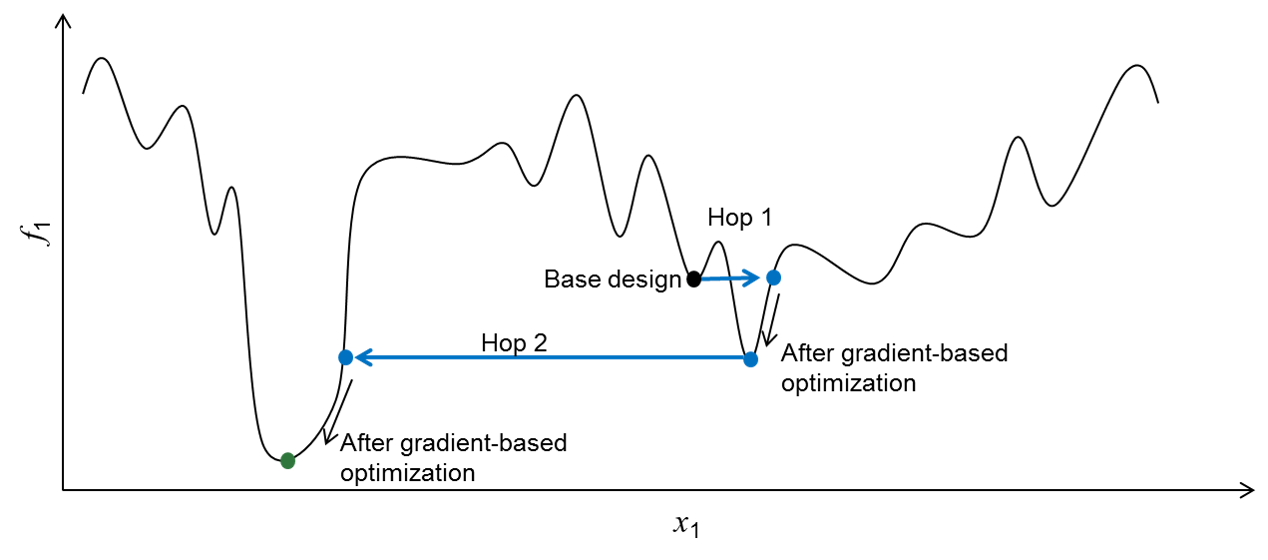
\includegraphics[width=0.8\linewidth]{MBH.png}
	\caption{ Monotonic Basin Hopping on a 1-dimensional function.}
	\label{fig:MBH}
\end{figure}

\ac{MBH} is run until either a specified number of iterations (trial points attempted) or a maximum CPU time is reached, at which point the best solution stored in the archive is returned. The version of \ac{MBH} used in EMTG has two parameters: the stopping criterion and the type of random step used to generate the perturbed decision vector $\mathbf{x}'$. In this work, the random step is drawn from a bi-directional Pareto distribution with the Pareto parameter, $\alpha$, set to 1.4. The bi-directional Pareto distribution usually generates small steps that allow \ac{MBH} to \textit{exploit} the local cluster around the current best solution. However, some of the steps generated by the bi-directional Pareto distribution are much larger, in some cases spanning the entire decision space. These larger steps allow \ac{MBH} to \textit{explore} the full decision space. This approach has been shown to be robust on complex interplanetary trajectory design problems \cite{MBH_ISSFD_2014}.

\ac{MBH} may be started either from a uniform-randomly chosen point in the decision space or from an initial guess derived from a previous problem. As long as the two problems are sufficiently similar, the latter approach is more efficient than starting from randomness. However, on simple problems, \ac{MBH} will quickly find the global best solution with or without an initial guess.

\section{Initial Guess}
\label{sec:initial_guess}

If the user chooses to specify an initial guess to \ac{MBH} or to run \ac{EMTG} in \ac{NLP}-only or evaluate-only mode, then an initial guess must be provided. \ac{EMTG} features an intelligent initial guess parser that is designed to minimize load on the user. This process is actually executed by the \texttt{Mission} class but is described here because this is where users would expect to find it. The initial guess parser obeys the following rules:

\begin{enumerate}
	\item The initial guess is specified at the Journey level, in the \texttt{trialX} field of each \texttt{JourneyOptions} object. The user may type or paste the initial guess into the corresponding \texttt{trialX} field for each journey in the .emtgopt input script.
	\item Each entry in the initial guess is a comma-separated tuple. The first element is the name of the decision variable and the second element is the value. The name of each decision variable can be found by running \ac{EMTG} with no initial guess and reading the resulting XFfile.csv that lists all decision variables and constraints.
	\item While \ac{EMTG}'s internal time calculations are performed in seconds, we recognize that humans like to think in days and so time variables in the initial guess are parsed in days.
	\item If any decision variable is \textit{not} specified, \ac{EMTG} will assign a uniform random number between the bounds of that variable. It is therefore possible to supply a partial initial guess. \ac{EMTG} warns the user when it does this.
	\item Decision variables related to a number of time steps, such as control variables in a \texttt{TwoPointShootingPhase} or state and control variables in a \texttt{ParallelShootingPhase} are interpolated to the number of time steps present in the phase. The user may specify an initial guess with a different number of time steps than the mission is configured for - \ac{EMTG} will figure it out.
	\item Decision variables in the initial guess whose names are not recognized are ignored.
\end{enumerate}

\chapter{Math}
\label{chap:math}

\section{Matrix}
\label{sec:EMTG_Matrix}

\ac{EMTG} performs all matrix and vector computations using the \texttt{EMTG\_Matrix} class. \texttt{EMTG\_Matrix} provides dense matrix functionality that is templated and can be used with regular double precision numbers, integers, booleans, or algorithmic differentiation calculation objects. For a full exhaustive list of methods available in \texttt{EMTG\_Matrix}, see the Doxygen output.

The developer may turn matrix error checking on and off at compile time. It is very useful to have this checking turned on during development but once code is fully developed and tested the error checking is removed for speed.

\section{Tensor}
\label{sec:EMTG_Tensor}

\texttt{EMTG\_Tensor} is similar to \texttt{EMTG\_Matrix} but for 3-tensors. \texttt{EMTG\_Tensor} implements fewer operations than \texttt{EMTG\_Matrix} because tensors are very rare in \ac{EMTG} and not many operations are needed. A full list of methods in \texttt{EMTG\_Tensor} is included in the Doxygen output.

\section{Interpolator}
\label{sec:EMTG_interpolator}

The \texttt{interpolator} class is a very simple linear interpolator that is used by \ac{EMTG} when parsing initial guesses. It operates on a \texttt{std::vector} of \texttt{std::pair} objects.

\section{EMTG math utilities and constants}
\label{sec:EMTG_math}

The \texttt{EMTG\_math.h} header contains mathematical constants and basic functions that do not fit anywhere else. These include:

\begin{itemize}
	\item Definitions of $\pi$, $\pi/2$, and $2\pi$.
	\item The conversion from degrees to radians.
	\item A definition of a ``small'' number in \ac{EMTG}, currently set to 1.0e-13.
	\item A definition of a ``large'' number in \ac{EMTG}, currently set to 1.0e+30.
	\item An \texttt{sgn()} function to find the sign of a value. Works for double, int, and algorithmic differenation overloaded computation objects.
	\item \texttt{acosh()} and \texttt{asinh()} functions, compatible with algorithmic differentiation.
	\item \texttt{safe\_acos()} and \texttt{safe\_asin()} functions that clip the input argument between 0.0 and 1.0 and so never fail, compatible with algorithmic differentation.
	\item A \texttt{norm()} function for \texttt{std::vector}, which is rarely used but sometimes helpful. Compatible with algorithmic differentation.
	\item An \texttt{absclip()} function to return a value clipped between plus or minus a user-supplied maximum absolute value. Compatible with algorithmic differentiation.
\end{itemize}

\section{RandUtils}
\label{sec:randutils}

\ac{EMTG} uses the \texttt{randutils} package by Melissa O'Neill to generate random numbers. This is the only third-party code that is distributed with the \ac{EMTG} code base, and is released under the MIT License. The license is included in its entirety at the beginning of \texttt{randutils.h}.

\chapter{Derivative Testbed}
\label{chap:testing}

One of the most challenging aspects of creating an optimization tool is the need to code, test, and maintain analytical derivatives of each of the objective functions and constraints with respect to the decision variables. This testing is often done with finite differencing or by creating stand-alone testbeds that use algorithmic differentiation or complex step differentiation via operator overloading. Neither of these methods is reliable because the former is subject to finite differencing rounding and truncation error and the latter introduces a risk of human error when re-coding a derivative from the stand-alone testbed to the main program code.

After many frustrating years of using both of the above methods, we decided to build \ac{EMTG} version 9 a very different way. The entire \ac{EMTG} version 9 code base is compatible with algorithmic differentation via the \ac{GSAD} package. All values that are used in the computation of a constraint or objective function are specified as \texttt{doubleType}, which in turn may be cast as \texttt{double} or \texttt{GSAD::adouble} depending on whether one is compiling in optimization mode or testbed mode.

The derivatives testbed executes \ac{EMTG} in ``evaluate trialX'' mode with algorithmic differentation available. The testbed prints out the following files:

\begin{itemize}
	\item \texttt{Mission\_XFout.csv} - Lists the decision variables and constraints along with their bounds and values. This is the same file that is written when executing \ac{EMTG} the normal way.
	\item \texttt{Mission\_Gout.csv} - Lists every single partial derivative of every nonlinear constraint and the objective function with respect to every decision variable in its sparsity pattern. Lists the analytical value, the algorithmic differentiation value, the relative and absolute errors, the ratios between the analytical and algorithmic values, the indices in the sparse Jacobian, and the order of magnitude of the derivative entry.
	\item \texttt{Mission\_Aout.csv} - Same as \texttt{Mission\_Gout.csv} but for linear constraints and objectives.
	\item \texttt{Mission\_MissingEntries.csv} - Lists the Jacobian indices and order of magnitude of any derivative entry that \textit{should} exist based on the derivative directions polled from each algorithmic differentation calculation object, but the programmer forgot to code.
\end{itemize}

The derivatives testbed allows a developer to trivially test a highly complex optimization problem and ensure that the derivatives are as correct as possible. The only complications are when an entry is so small that the true value is obscured by floating point chaos.

Developers may also construct smaller-scale derivatives testbeds that test only portions of \ac{EMTG}. The repository includes testbeds for boundary events, propagation, the \ac{MGALT} \ac{STM}-\ac{MTM} chain, and frame rotations. These secondary testbeds are not maintained like the main testbed and are provided only as examples of how to make tests.

\chapter{Regression Testbed}
\label{chap:testing}

\hl{Alec and Sean}

\section{Comparatron Function}
\label{sec:comparatronfunction}

\texttt{Comparatron} is a method of the PyEMTG \texttt{Mission} class which compares all EMTG output attributes against those of a baseline case. Strings are compared directly and numeric values are checked against a default tolerance of 1e-15. Alternative tolerance values for any attribute can be provided as a dictionary into the function. If all values are in agreement, \texttt{Comparatron} returns a boolean value ``True". If any values are not within the tolerance between the two cases, then a value of ``False" is returned along with a csv output file of all values that do not match.

Since \texttt{Comparatron} is written entirely in Python, all classes referenced in this section are PyEMTG classes, not EMTG C++ classes.

The syntax for calling \texttt{Comparatron} is: ``$pass\_test=myMission.Comparatron(path\_to\_baseline,\linebreak csv\_file\_name=None,full\_output=False,tolerance\_dict=\{\},default\_tolerance=$1e-15$)$.'' Note that this is Python syntax. Any argument with an ``='' sign denotes the default value that will be used if the argument is not passed in. The function arguments are as follows:
\begin{itemize}[label=$\bullet$]
	\item $path\_to\_baseline$: The full file path to the EMTG output file to compare against. This is the only required argument.
	\item $csv\_file\_name$: The name of the csv output file that is written if there are any discrepancies to report. If no file name is provided then the mission name will be used.
	\item $full\_output$: Dictates what is written to the csv output file. If False, only values that do not meet the tolerance will be written to the output. If True, than any values that are not in exact agreement (regardless of whether they are within the tolerance) will be written. 
	\item $tolerance\_dict$: Overrides the default tolerance for specific mission, journey, or mission event attributes. The argument takes a dictionary with the attribute as the key and the new tolerance as the value (i.e. \{`total\_statistical\_deltav':1e-6,`Declination':1e-8\}).
	\item $default\_tolerance$: Provides a default tolerance value for all attributes that do not appear in the tolerance dictionary. A value of 1e-15 will be used unless the user provides a new default value here.
\end{itemize}

When running \texttt{Comparatron}, the function will first check to make sure that both cases have the same number of journeys and mission events. If there are discrepancies in either, the function will not return the usual True/False boolean but will instead return a string saying ``Journey Mismatch" or ``Journey \# Mission Events Mismatch" and will stop immediately. If this check is passed, \texttt{Comparatron} will then check every \texttt{Mission}, \texttt{Journey}, and \texttt{MissionEvent} class attribute across cases and record any names that do not agree or any attributes that appear only in one---these will be written to the csv output file. The attributes for each class include both functions within the class as well as alphanumeric values (i.e. dates, the central body, and $\Delta v$). All alphanumeric-valued attributes are parsed into a temporary dataframe for the overall mission and for each journey and mission event. These temporary dataframes are split in two, one for strings and one for numerics. The strings are compared directly while the corresponding numeric dataframes between the two EMTG cases are subtracted and checked against the tolerance. All values that do not completely agree are stored into a final comparison dataframe, which gets written to a csv output file if discrepancies are found.

\bibliographystyle{AAS_publication}
\bibliography{EMTGbib}

\end{document}





















